\documentclass[10pt, landscape]{article}
\usepackage[scaled=0.92]{helvet}
\usepackage{multicol}
\usepackage{calc}
\usepackage{ifthen}
\usepackage[landscape]{geometry}
%\usepackage{hyperref}

\usepackage{newtxtext} 

%for strikeout
\usepackage{ulem}

%For editing parbox
\usepackage[table]{xcolor}
%For editing itemise margins, reduce iterm separaion and list separation
\usepackage{enumitem}
% For math
\usepackage{amsmath,amsthm,amsfonts,amssymb}

%For pictures / figures
\usepackage{color,graphicx,overpic}
\graphicspath{ {./images/} }

%\usepackage{newtxtext} 
%\usepackage{amssymb}
%\usepackage[table]{xcolor}
%\usepackage{vwcol}
%\usepackage{tikz}
%\usepackage{wrapfig}
%\usepackage{makecell}

\pdfinfo{
  /Title (CS3223-notes.pdf)
  /Creator (Ger Teck)
  /Author (Ger Teck)
  /Subject ()
  /Keywords (tex)}

%% Margins for PAPER

% This sets page margins to .5 inch if using letter paper, and to 1cm
% if using A4 paper. (This probably isn't strictly necessary.)
% If using another size paper, use default 1cm margins.
\ifthenelse{\lengthtest { \paperwidth = 11in}}
	{ \geometry{top=.3in,left=.3in,right=.3in,bottom=.3in} }
	{\ifthenelse{ \lengthtest{ \paperwidth = 297mm}}
		{\geometry{top=0.5cm,left=0.5cm,right=0.5cm,bottom=0.5cm} }
		{\geometry{top=0.5cm,left=0.5cm,right=0.5cm,bottom=0.5cm} }
	}

% Turn off header and footer
\pagestyle{empty}
% for tight centres (less spacing)
\newenvironment{tightcenter}{%
  \setlength\topsep{0.5pt}
  \setlength\parskip{0.5pt}
  \begin{center}
}{%
  \end{center}
}

% Redefine section commands to use less space
\makeatletter
\renewcommand{\section}{\@startsection{section}{1}{0mm}%
                                {-1ex plus -.5ex minus -.2ex}%
                                {0.5ex plus .2ex}%x
                                {\normalfont\large\bfseries}}
\renewcommand{\subsection}{\@startsection{subsection}{2}{0mm}%
                                {-1explus -.5ex minus -.2ex}%
                                {0.5ex plus .2ex}%
                                {\normalfont\normalsize\bfseries}}
\renewcommand{\subsubsection}{\@startsection{subsubsection}{3}{0mm}%
                                {-1ex plus -.5ex minus -.2ex}%
                                {1ex plus .2ex}%
                                {\normalfont\small\bfseries}}
% change font
%\renewcommand{\familydefault}{\sfdefault}
%\renewcommand\rmdefault{\sfdefault}
\linespread{1.05}

\makeatother

% Define BibTeX command
\def\BibTeX{{\rm B\kern-.05em{\sc i\kern-.025em b}\kern-.08em
    T\kern-.1667em\lower.7ex\hbox{E}\kern-.125emX}}

% Don't print section numbers
\setcounter{secnumdepth}{0}

\setlength{\parindent}{0pt}
\setlength{\parskip}{0pt plus 0.5ex}

%% this changes all items (enumerate and itemize, reduce margins) ITEMIZE SEPARATION HERE
\setlength{\leftmargini}{0.5cm}
\setlength{\leftmarginii}{0.5cm}
\setlist[itemize,1]{leftmargin=2mm,labelindent=1mm,labelsep=1mm, itemsep = 0mm}
\setlist[itemize,2]{leftmargin=4mm,labelindent=1mm,labelsep=1mm, itemsep = 0mm}

%itemsep = 0mm
%\setlist{nosep}

% For Code Blocks
\usepackage{xcolor}
\usepackage{listings}

\lstdefinestyle{mystyle}{
	backgroundcolor=\color{gray!25!white},
	basicstyle=\scriptsize,
	numbers=none,    %or = none or left
	showstringspaces=false,
	breaklines=true,
	breakatwhitespace=false,                  
	captionpos=b,                    
	keepspaces=true,                                 
	numbersep=5pt,                  
	showspaces=false,                
	showtabs=false,                  
	tabsize=2,
 }
%Helpful:
%[linewidth = 1.0 \linewidth]
%\lstinline{}
% use \code{} for \lstinline with colorbox.
\newcommand{\code}[1]{\colorbox{gray!25!}{\lstinline|#1|}}
\lstset{style=mystyle}


% -------------------------------------------------------------------------------

% START OF DOCUMENT HERE

\begin{document}
\raggedright
\footnotesize
\begin{multicols*}{3}

% multicol parameters
% These lengths are set only within the two main columns
%\setlength{\columnseprule}{0.25pt}
\setlength{\premulticols}{1pt}
\setlength{\postmulticols}{1pt}
\setlength{\multicolsep}{1pt}
\setlength{\columnsep}{2pt}

%% DOCUMENT NAME HERE
\begin{center}
     \Large{\textbf{CS3223 Database Systems Implementation}} \\
\end{center}
AY23/24 Sem 2, github.com/gerteck


\section{Introduction}

\subsubsection{Course Details}
\begin{itemize}
\item Prerequisite knowledges: CS2040S, CS2102, CS2106 background (helpful).
\item Reference Textbook: Raghu \& Johannes Database M. Systems, 2002. \\
Encouraged to read ahead based on schedule before the lecture.
\item Course covers data structures, algorithms, different components making up database systems.
\end{itemize}

\centerline{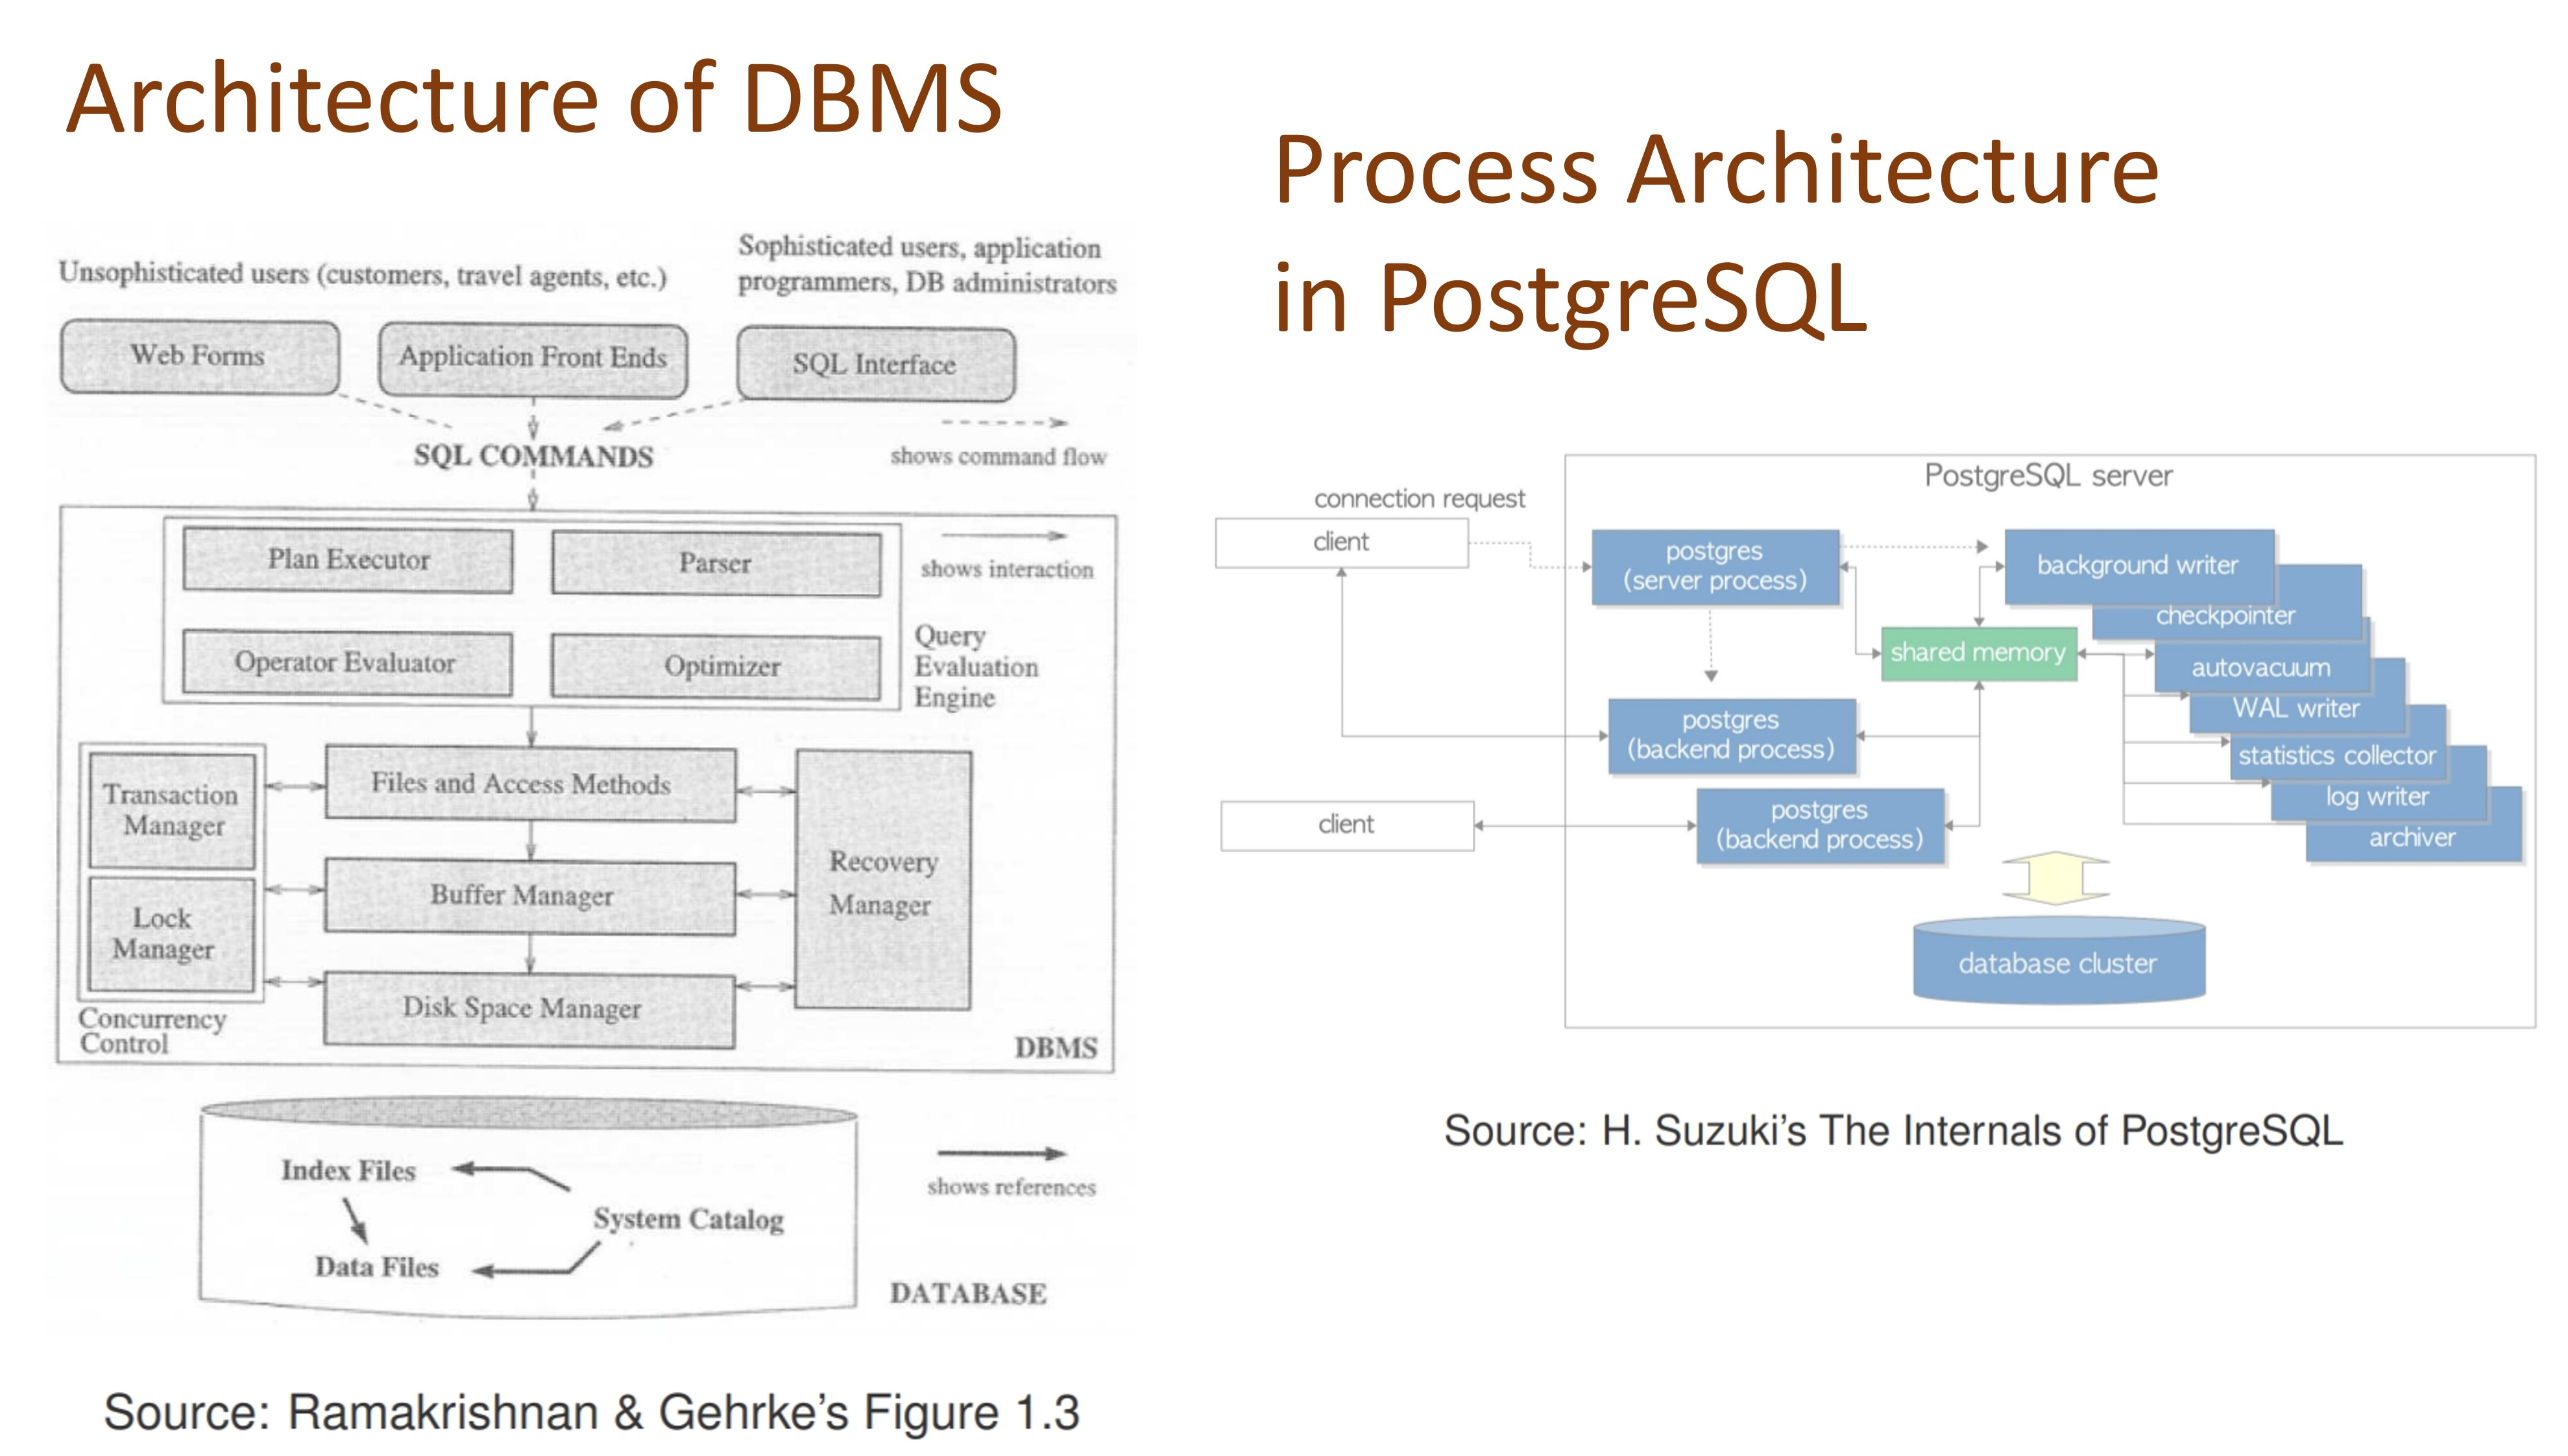
\includegraphics[width = 0.9\linewidth]{DBMSArchitecture}}

\begin{itemize}
\item OLTP: Online Transaction Processing is a type of data processing that consists of executing a number of transactions occurring concurrently—online banking, shopping, order entry, or sending text messages, for example.
\item OLAP: Online Analytical Processing.
\item Focusing on centralized database running on a single server.
\end{itemize}

\section{1. Data Storage}
\textbf{References}: R\&G Chapt 8. (Storage \& Indexing Overview), Chapt 9. (Storing Data: Disks and Files).

\subsubsection{A DBMS stores}
\begin{itemize}
\item Relations (Actual tables)
\item System catalog (aka data dictionary) storing metadata about relations.  \\
(Relation schemas, structure of relations, constraints, triggers. View definitions, Indexes - derived info to speed up access to relations, Statistical information about relations for use by query optimizer.) 
\item Log files: Information maintained for data recovery.
\end{itemize}

\subsubsection{DBMS Storage}
\textbf{Memory Hierarchy}: Primary (registers, RAM), secondary (HDD, SSD), tertiary memory with capacity / cost / access speed / volatility tradeoffs.
\begin{itemize}
\item DBMS stores data on non-volatile disk for persistence.
\item DBMS processes data in main memory (RAM).
\item Disk access operations (I/O). Read: transfer data from disk to RAM. Write: transfer data from RAM to disk.
\item Make use of index to speed up access, so that don't have to retrieve all the data when you run a query. Retrieve index and read only the block that contains specified data. Minimize I/O cost.
\end{itemize}

\subsubsection{Magnetic Hard-Disk Drive HDD}
\centerline{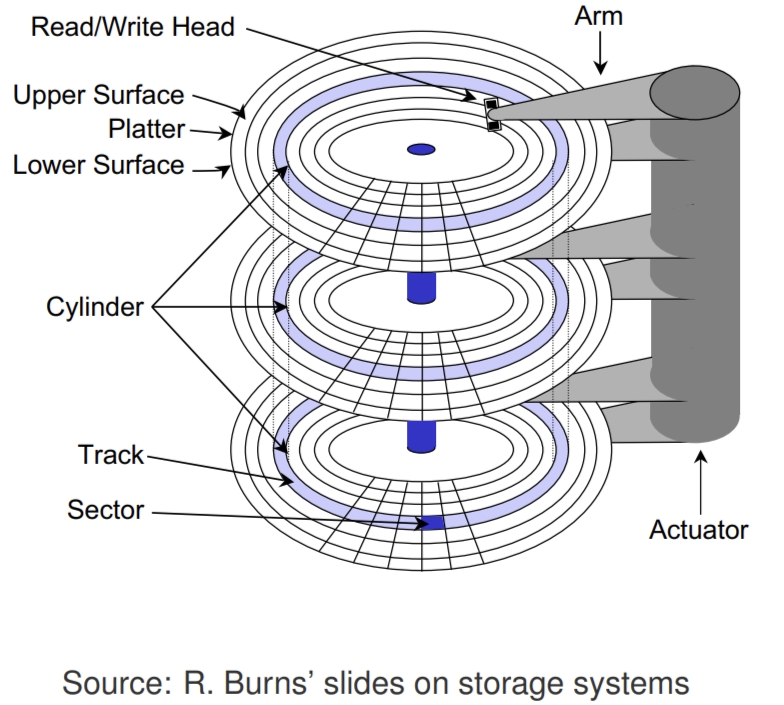
\includegraphics[width = 0.5\linewidth]{HDD}}
\begin{itemize}
\item Cylinder, Track, Sector: Units of the HDD storage system. To read from different tracks, need to move the mechanical HDD arm.
\item \textbf{Disk Access Time}:
	\begin{itemize}
		\item command processing time: interpreting access command by disk controller.
		\item seek time: moving arms to position disk head on track.
		\item rotational delay: waiting for block to rotate under head.
		\item transfer time: actually moving data to/from disk surface.
		\item \textbf{access time}: = seek time + rotational delay + transfer time. (CPT considered negligible). 
	\end{itemize}
\centerline{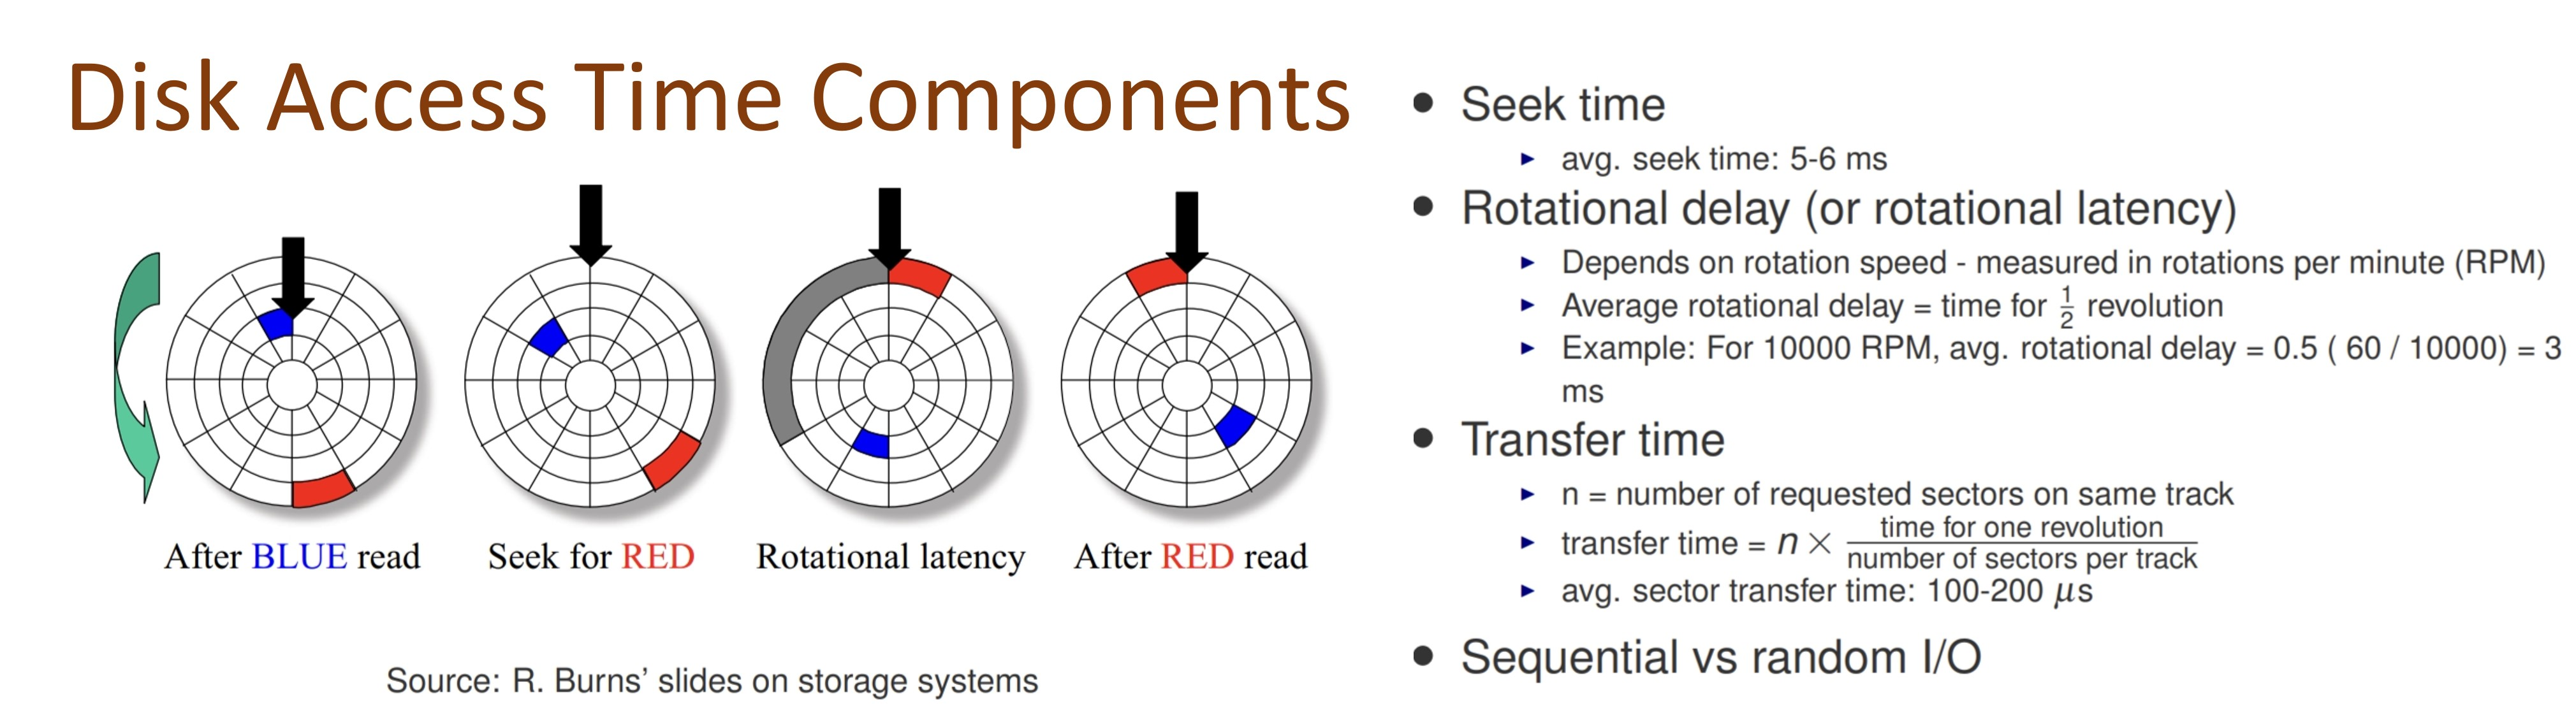
\includegraphics[width = 1\linewidth]{diskAccessTime}}
\item \textbf{Concept of Sequential vs random I/O.} \\
- \textbf{Sequential:} Both sector on same track. \\
- \textbf{Random:} Sectors on different track, require seeking (moving arm).
\item Given a set of data, we hope to store the data contiguously, on the same track. (Minimize incurring random I/O). If data is too large, store on same track, but different surface (aka same cylinder).
\item Complexity hidden to OS by disk controller. Shown as a sequence of memory locations.
\end{itemize}

\subsubsection{Solid-State Drive: SSD}
\begin{itemize}
\item Build with NAND flash memory without any mechanical moving parts. Lower power consumption.
\item \textbf{Random I/O}: 100x faster than HDD. (no moving parts)
\item \textbf{Sequential I/O}: slightly faster than HDD (~ 2x)
\item \textbf{Disadvantages}: update to a page requires erasure of multiple pages (~ 5ms) before ovewriting page. Limited number of times a page can be erased (~ $10^{5} - 10^{6}$)
\end{itemize}

\subsubsection{Storage Manager Components}
\begin{itemize}
\item Data is stored, retrieved in units called \textbf{disk blocks (or pages}. (Each block = sequence of one or more contiguous sectors.
\item \textbf{FIles \& access methods layer (aka file layer)} - deals with organization and retrieval of data.
\item \textbf{Buffer Manager} - controls reading/writing of disk pages.
\item \textbf{Disk Space Manager} - keeps track of pages used by file layer.
\end{itemize}
\centerline{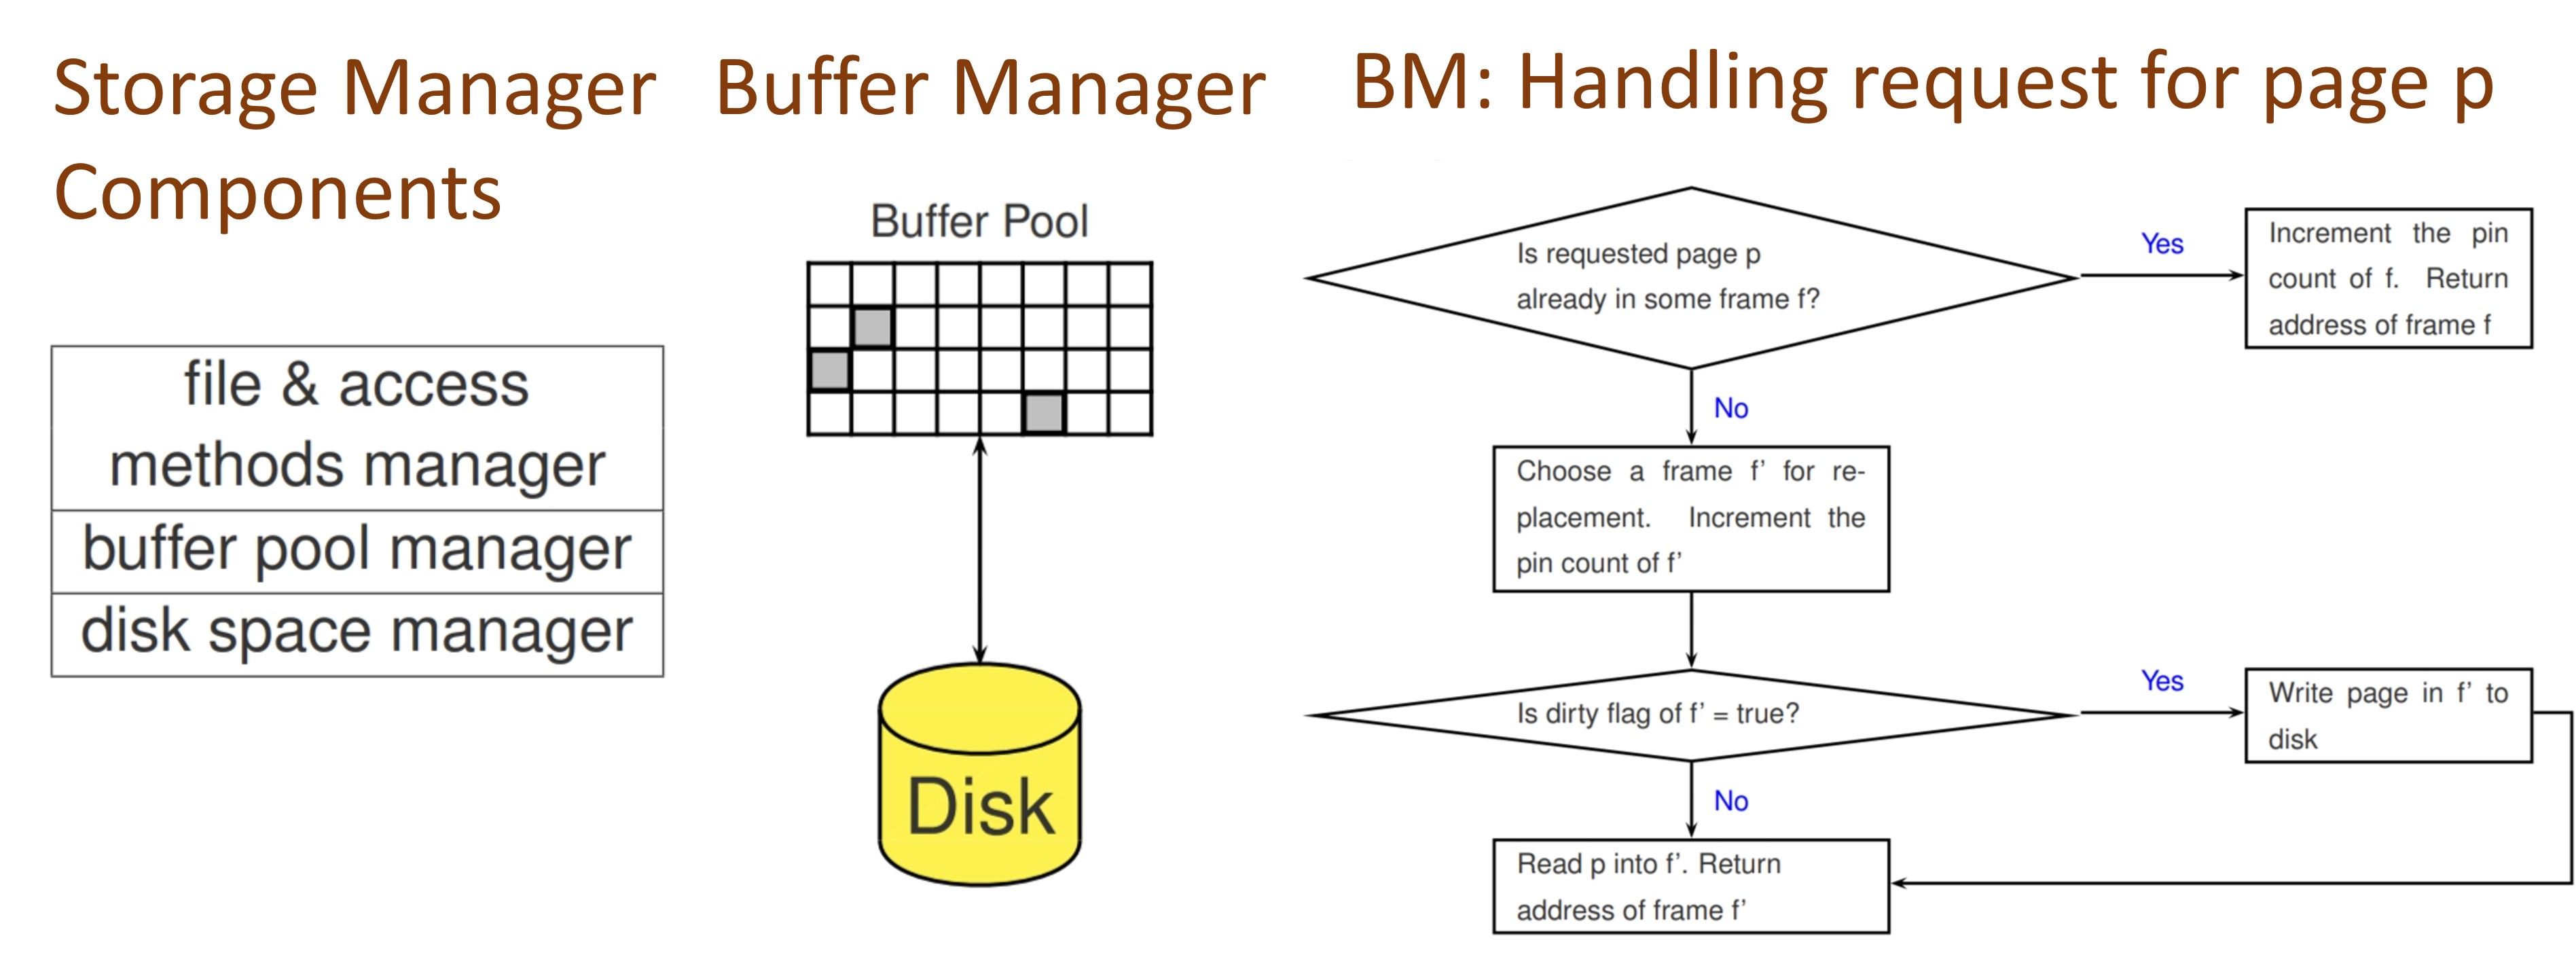
\includegraphics[width = 1\linewidth]{bufferManager}}


\textbf{Buffer Manager}
\begin{itemize}
\item \textbf{Buffer pool}: Main memory allocated for DBMS.
\item Buffer pool is partitioned into block-sized pages called \textbf{frames}.
\item Clients of buffer pool can request for disk page to be fetched into buffer pool, release a disk page in buffer pool.
\item A page in the buffer is \textbf{dirty} if it has been modified \& not updated on disk.
\item \textbf{Two variables} maintained for each frame in buffer pool: 
	\begin{itemize}
		\item \textbf{pin count}: number of clients using page (initialized 0)
		\item \textbf{dirty flag}: whether page is dirty (initialized false)
	\end{itemize}
\item Free list: Keeps track of frames that are free / empty.
\item \textbf{Pin count}: \\
- Incrementing pin count is \textbf{pinning} the requested page in its frame. \\
- Decrementing is \textbf{unpinning} the page. 
	\begin{itemize}
		\item Unpinning a page, dirty flag should be updated to true if page is dirty.
		\item A page in buffer can be replaced only when pin count is 0. 
		\item Before replacing buffer page, needs to be written back to disk if its dirty flag is true. 
	\end{itemize}
\item Buffer manager coordinates with transaction manager to ensure data correctness and recoverability.
\item \textbf{Replacement Policies}
	\begin{itemize}
		\item Replacement policy: Deciding which unpinned page to replace. (some examples:)
		\item Random, FIFO, Most Recently Used (MRU), Least Recently Used (LRU): (Use queue of pointers to frames with pin count = 0), most common, makes use of temporal locality.
		\item \textbf{Clock}: cheaper popular variant of LRU \\
		- \textbf{current} variable: points to some buffer frame. \\
		- Each frame has a \textbf{referenced bit}, turns on when its pin count turns 0. \\
		- Replace a page that has referenced bit off \& pin count = 0.
	\end{itemize}
\centerline{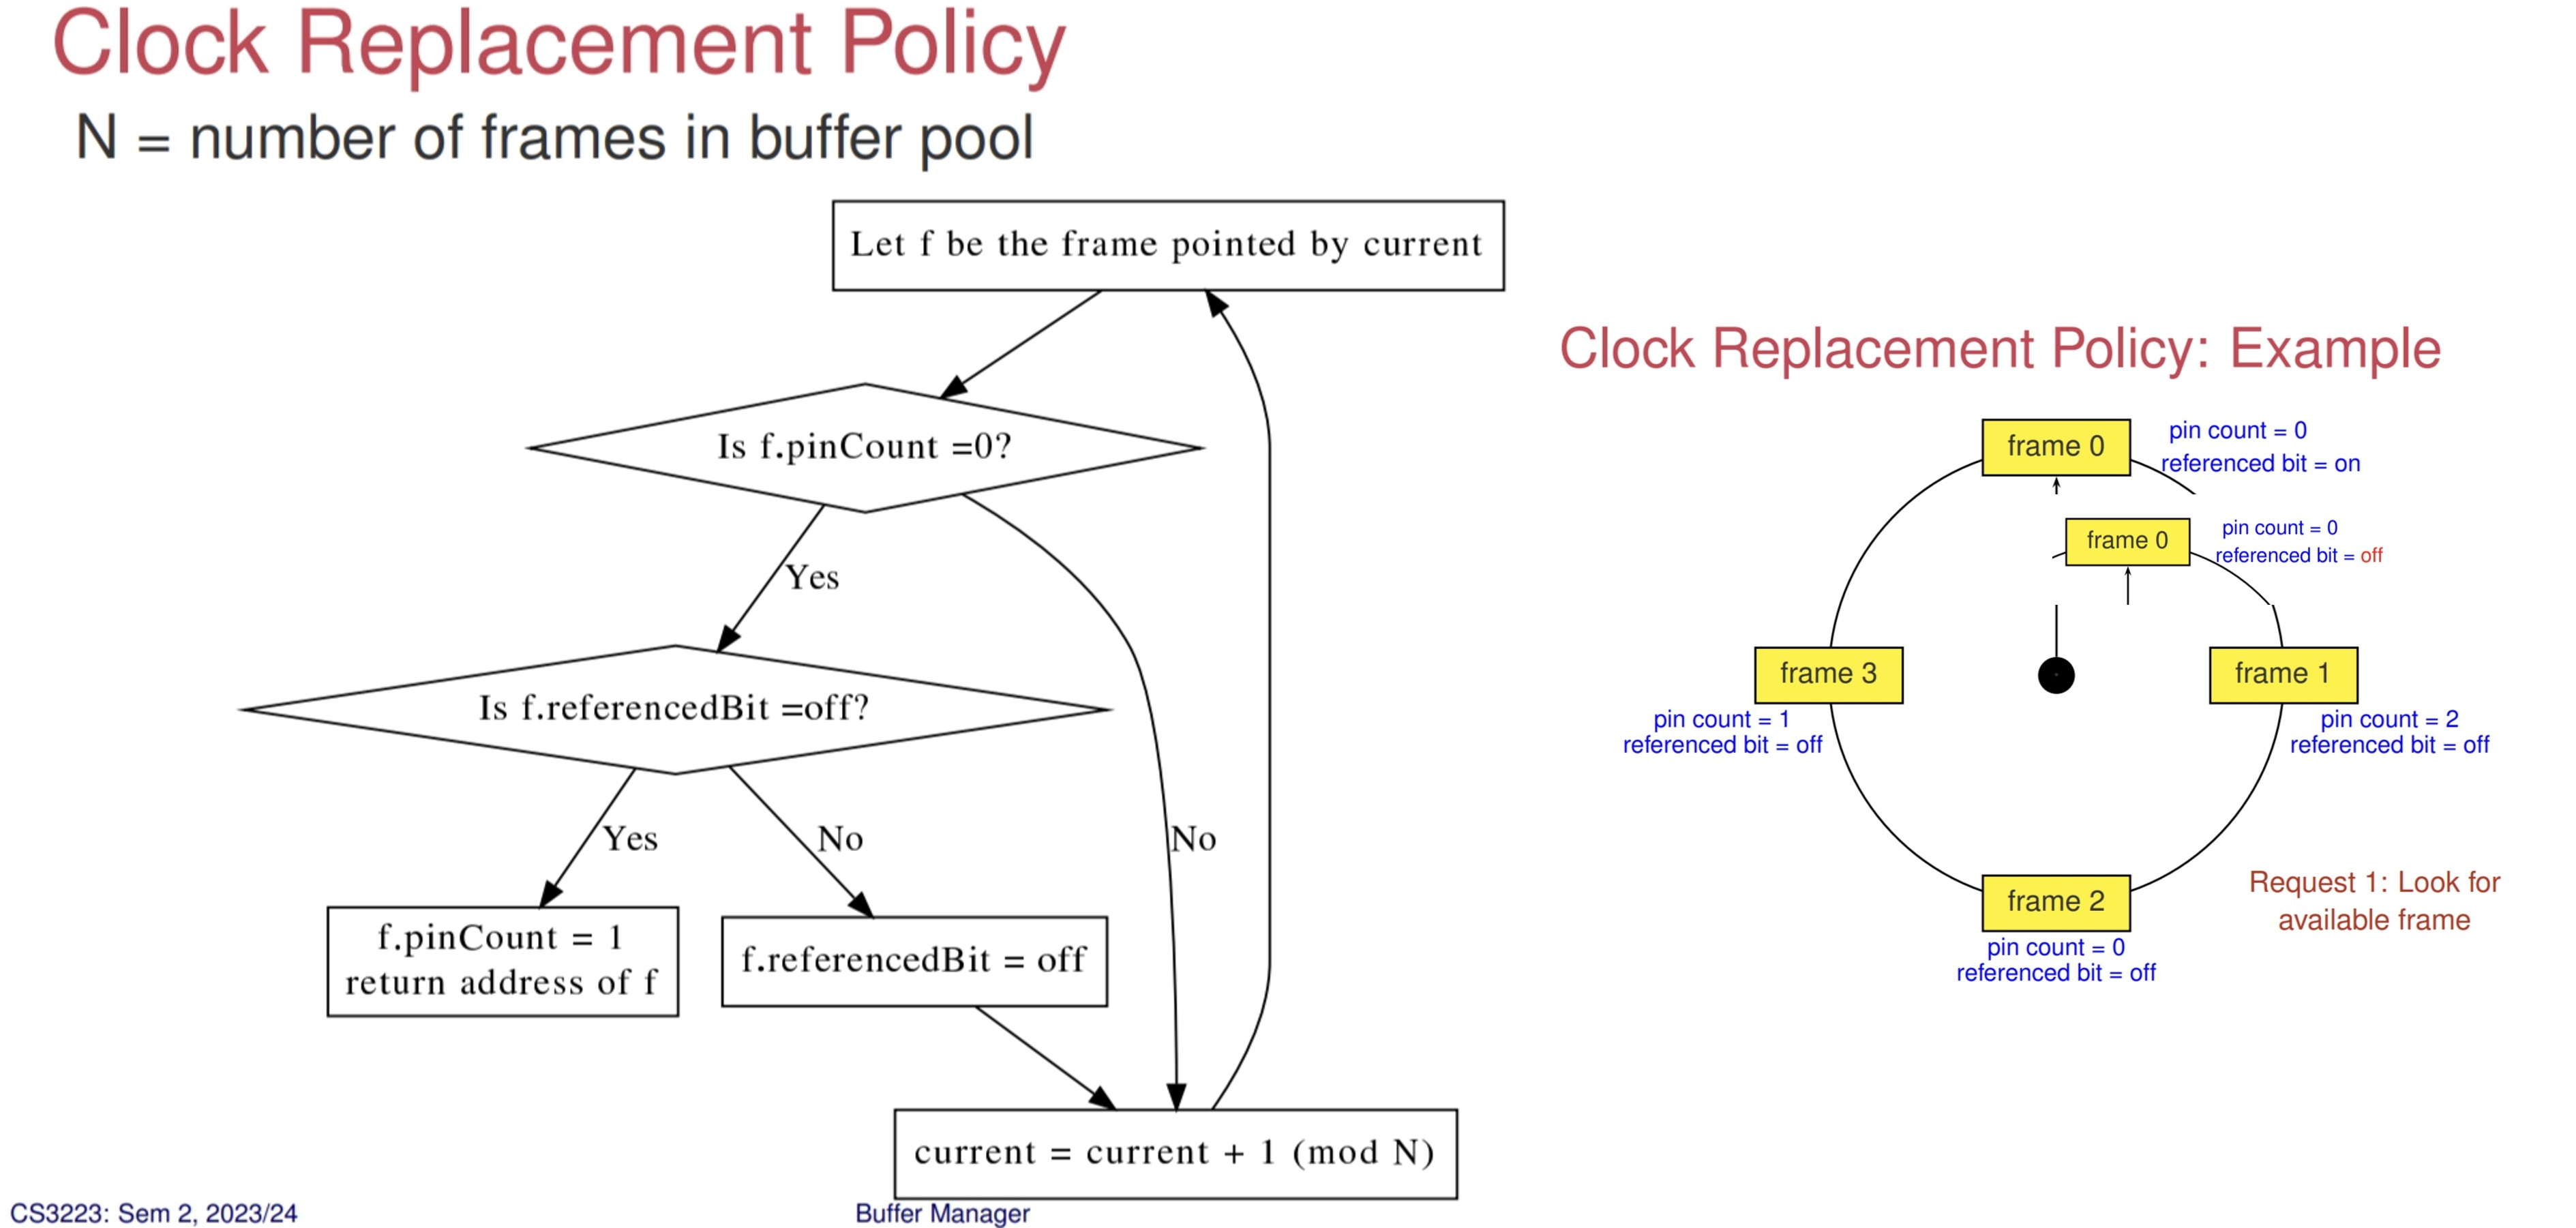
\includegraphics[width = 1\linewidth]{clockReplacementPolicy}}
\end{itemize}

\columnbreak

\subsection{Files}
\textbf{File Abstraction}
\begin{itemize}
	\item Each relation is a file of records.
	\item Each record has a unique record identifier called RID / TID.
	\item Common file operations: create/delete file, insert record, delete/get record with given RID, scan all records.
\end{itemize}
\textbf{File Organization}: Method of arranging data records in a file that is stored on disk.
\begin{itemize}
	\item \textbf{Heap file}: Unordered file
	\item \textbf{Sorted file}: Records order on some search key.
	\item \textbf{Hashed file}: Records located in blocks via a hash function.
\end{itemize}

\subsubsection{Heap File Implementations}
\centerline{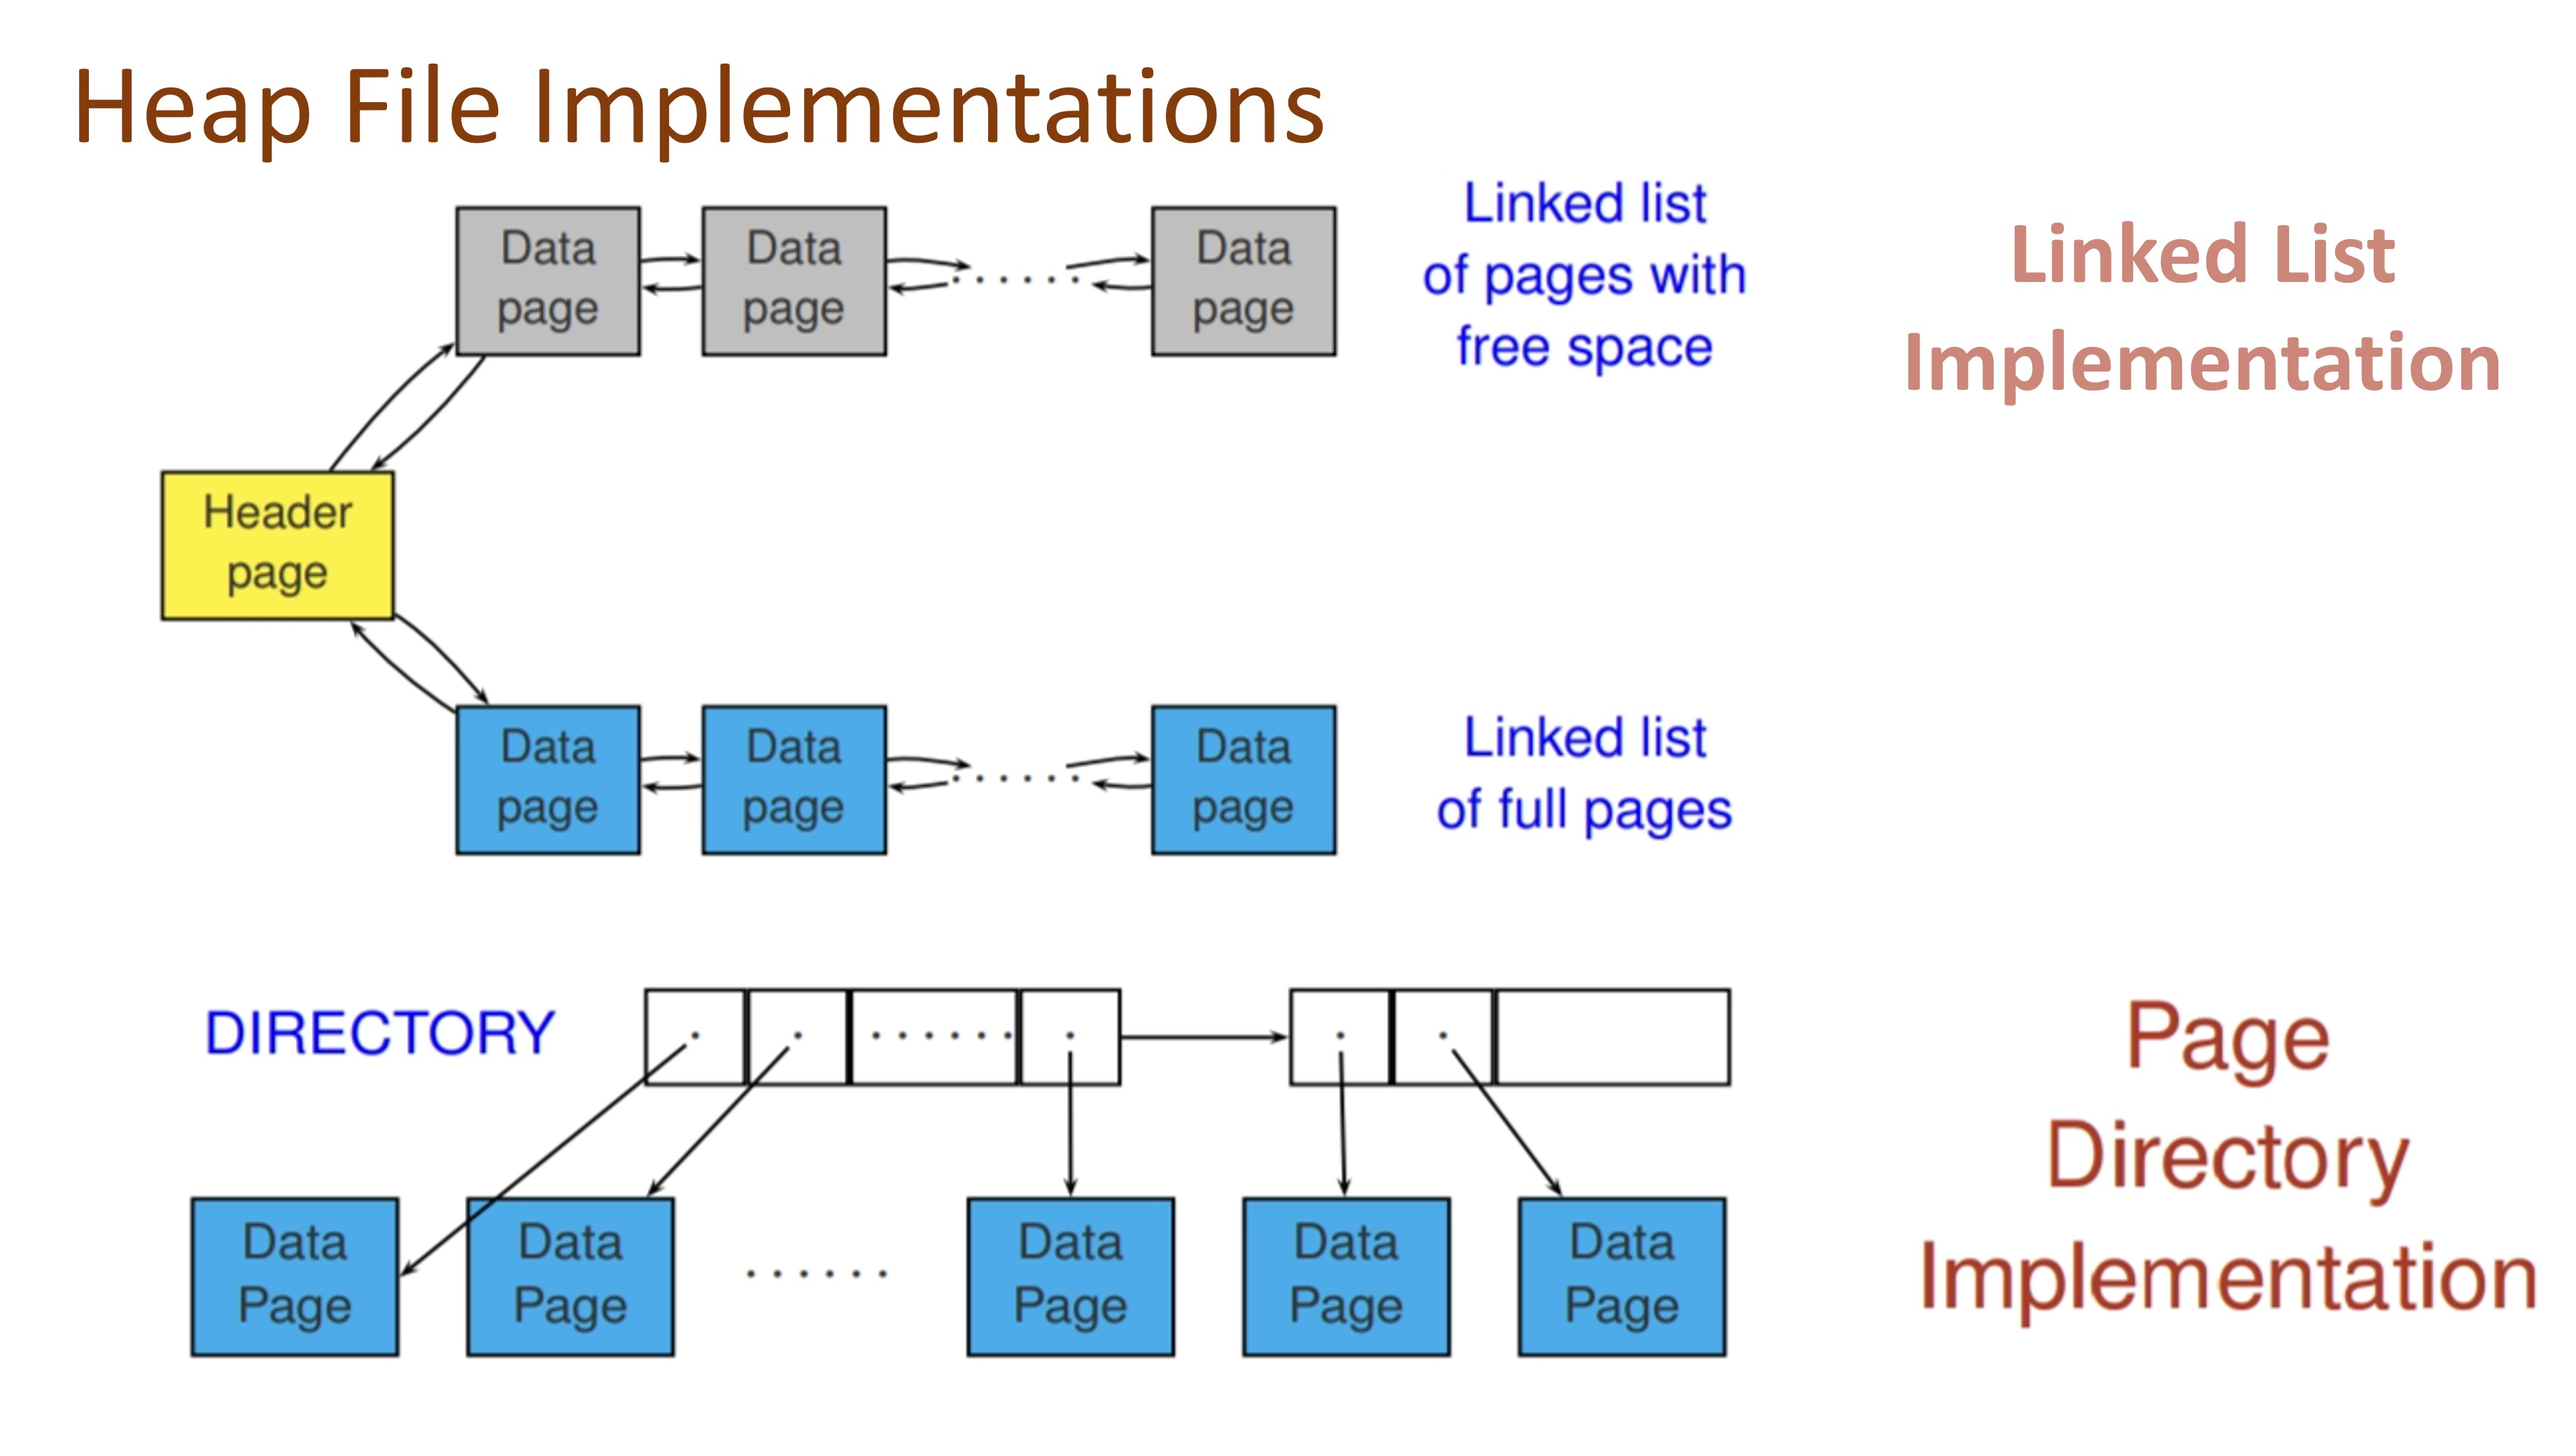
\includegraphics[width = 0.7\linewidth]{heapFileImplementations}}
\begin{itemize}
\item \textbf{Linked list implementation}: Two linked lists, one with pages with free space, other of completely full pages.
\item \textbf{Page Directory Implementation}: Two leveled implementation. Each big block is a disk block with some metadata. Each disk block has a number of data pages.
\end{itemize}

\textbf{Page Formats}: \\
Records are organized within a page and referenced with the RID.
\begin{itemize}
\item \textbf{RID = (page id, slot number)}
\item For \textbf{Fixed-Length Records}, Organization can be:
\begin{itemize}
\item \textbf{Packed Organization}: Store records in contiguous slots. 
\item  For packed organization, memory organization is tough and costly when record in slot is deleted, need to move up a record. But as RID serves as a reference, but need to propagate change in RID.
\item \textbf{Unpacked Organization}: Uses bit array to maintain free slots.
\item For unpacked organization, more bookkeeping needed (use bitmap, 1 \& 0 to check if occupied) to store records.
\end{itemize}
\item For \textbf{Variable-Length Records}: We could assume some maximum size, then use packed organization. But wasteful. Instead, we can use \textbf{Slotted Page Organization}.
\end{itemize}
\centerline{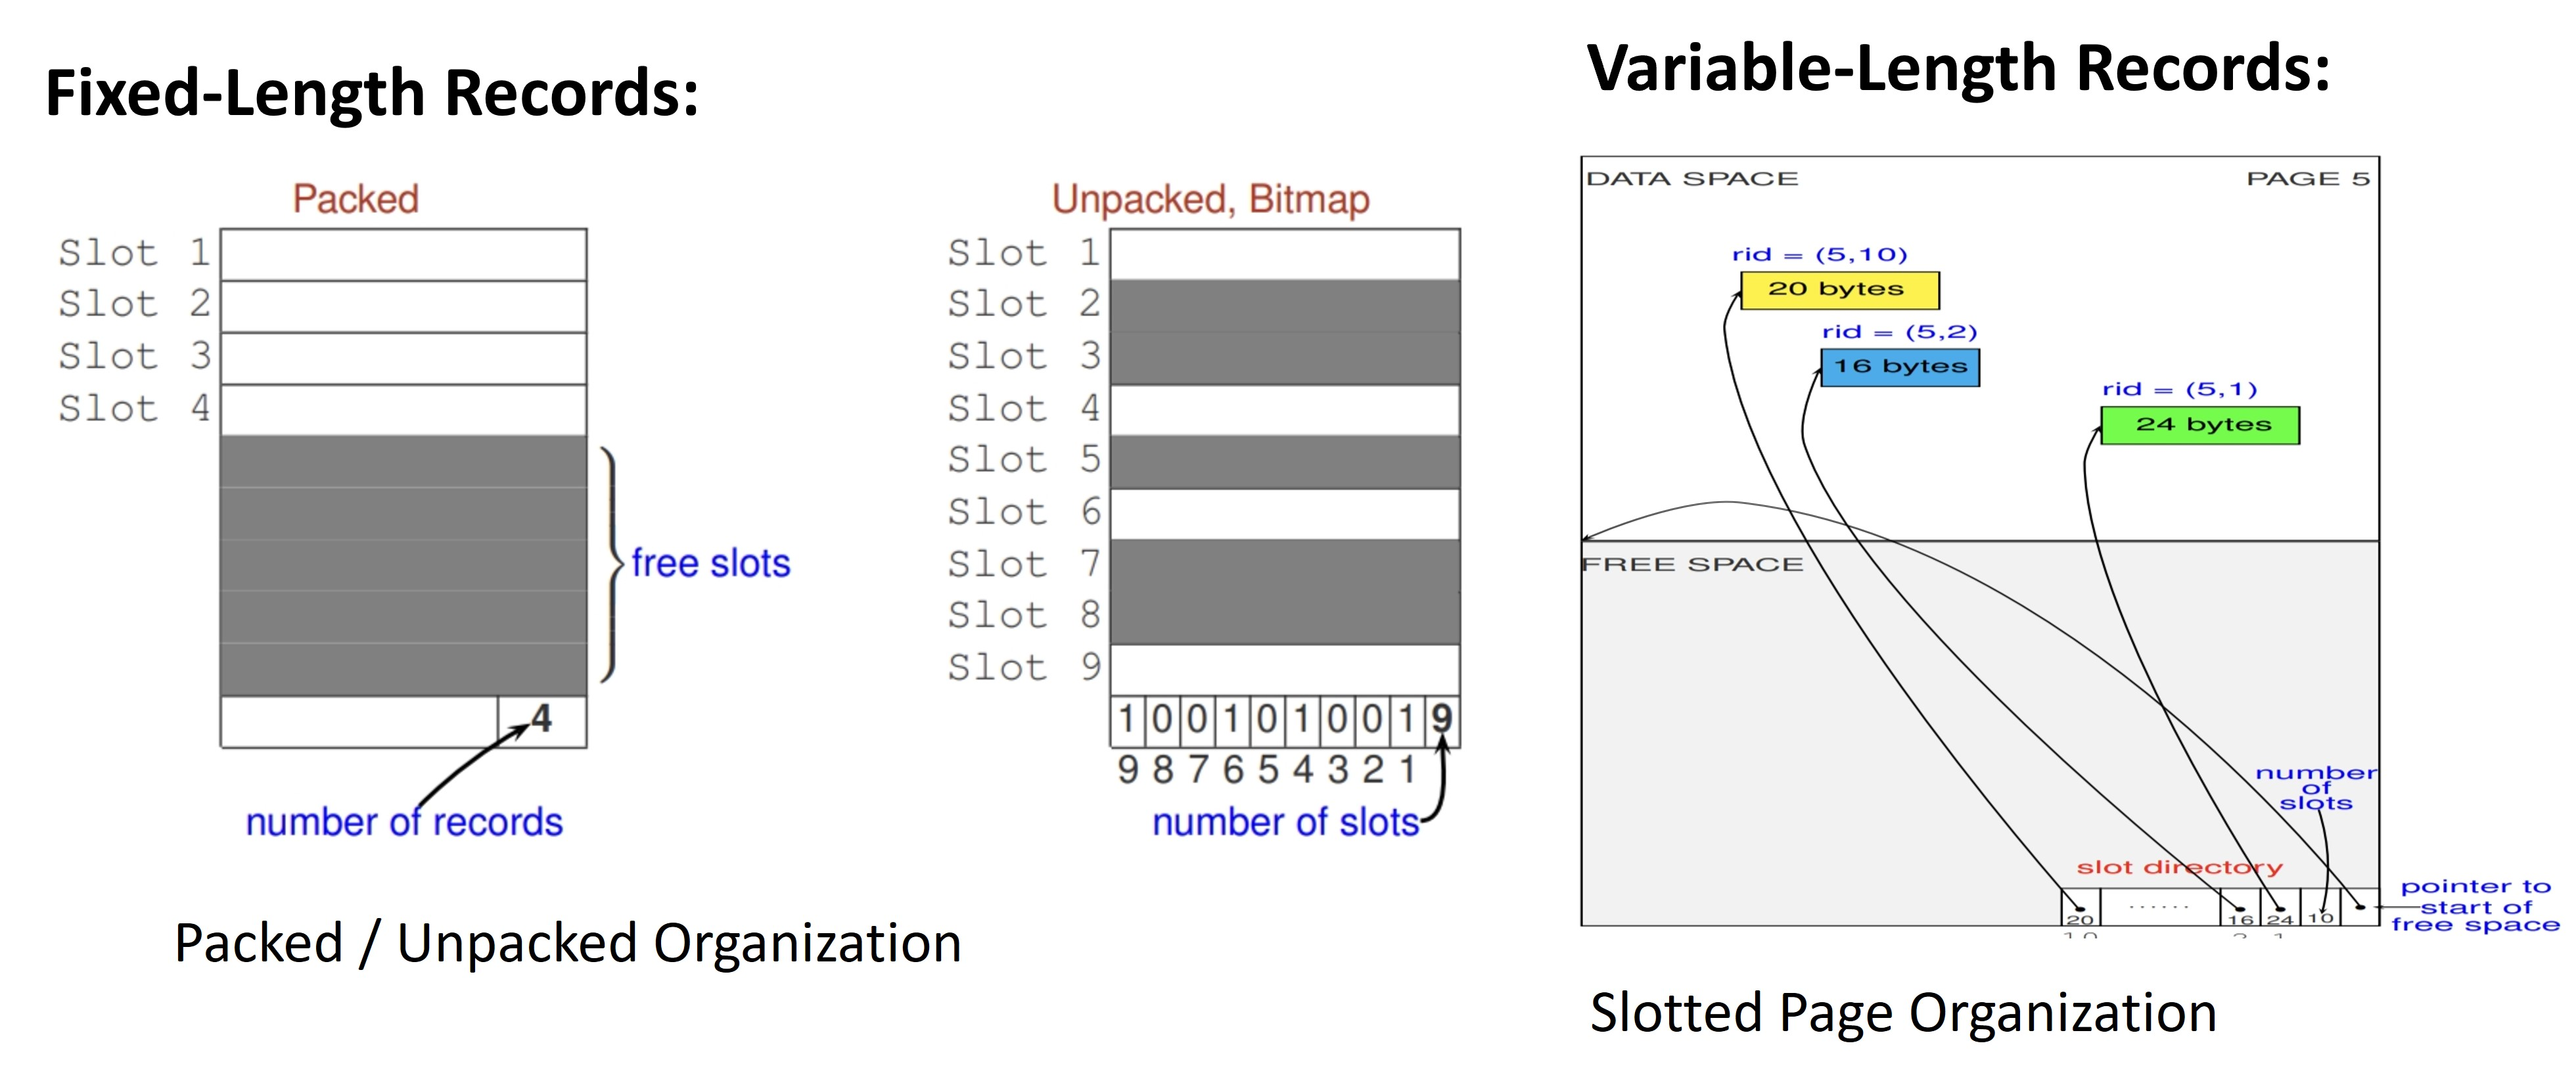
\includegraphics[width = 1\linewidth]{pageFormats}}

\centerline{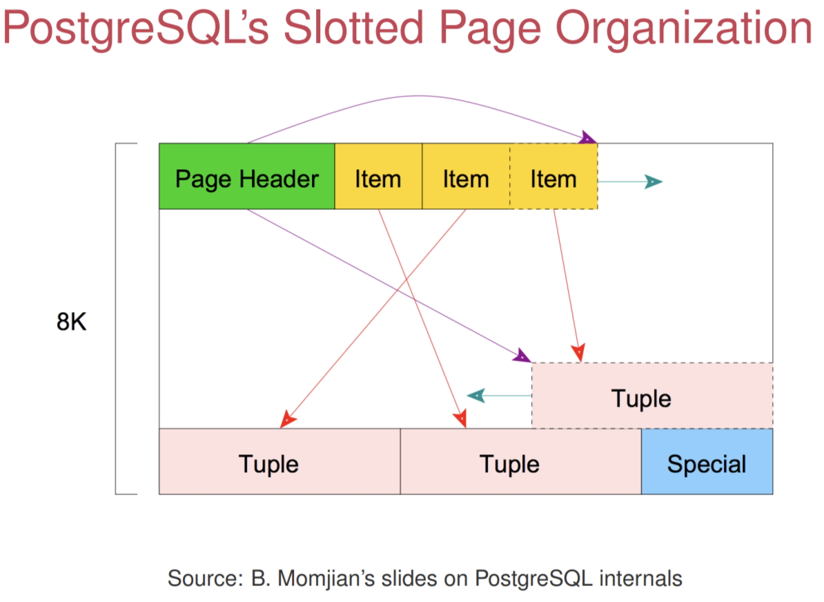
\includegraphics[width = 0.7\linewidth]{PostgreSQLPageOrg}}
\textbf{Record Formats}: Organizing fields within a record. \\
\medskip
\centerline{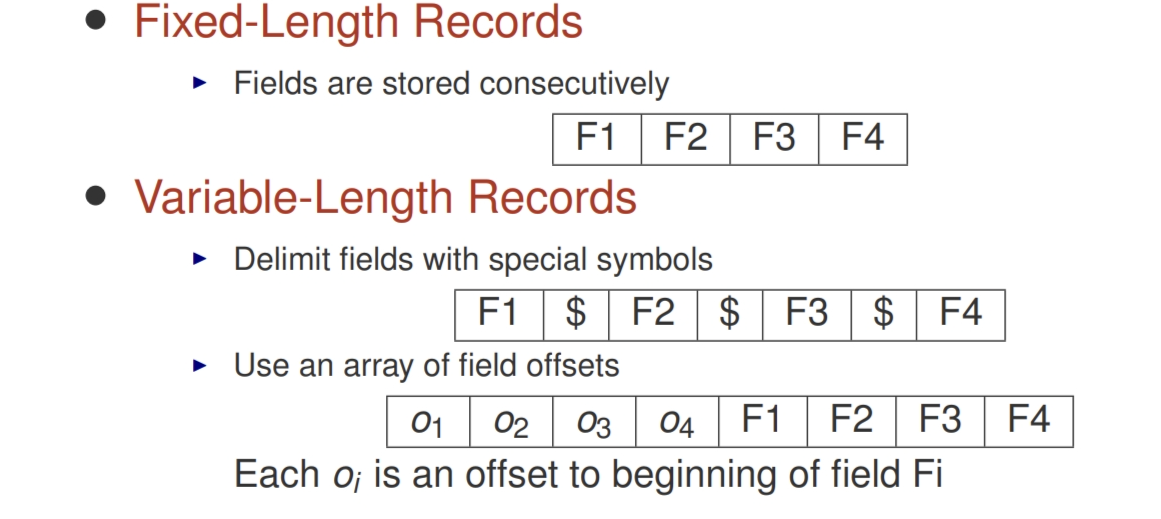
\includegraphics[width = 0.8\linewidth]{recordFormats}}

\section{2. Indexing}
Need some auxiliary data structure to make efficient queries.

\subsection{Index}
\begin{itemize}
\item An \textbf{index} is a data structure to speed up retrieval of data records based on some search key.
\item A \textbf{search key} is a sequence of $k$ data attributes, $k \geq 1$. (A search key is aka \textit{composite search key} if $k > 1$, e.g. (state, city).)
\item An index is a \textbf{unique index} if search key is a candidate key, otherwise it is \textbf{non-unique index}.
\item An index is stored as a file, records in index file referred to as \textbf{data entries}.
\end{itemize}
\centerline{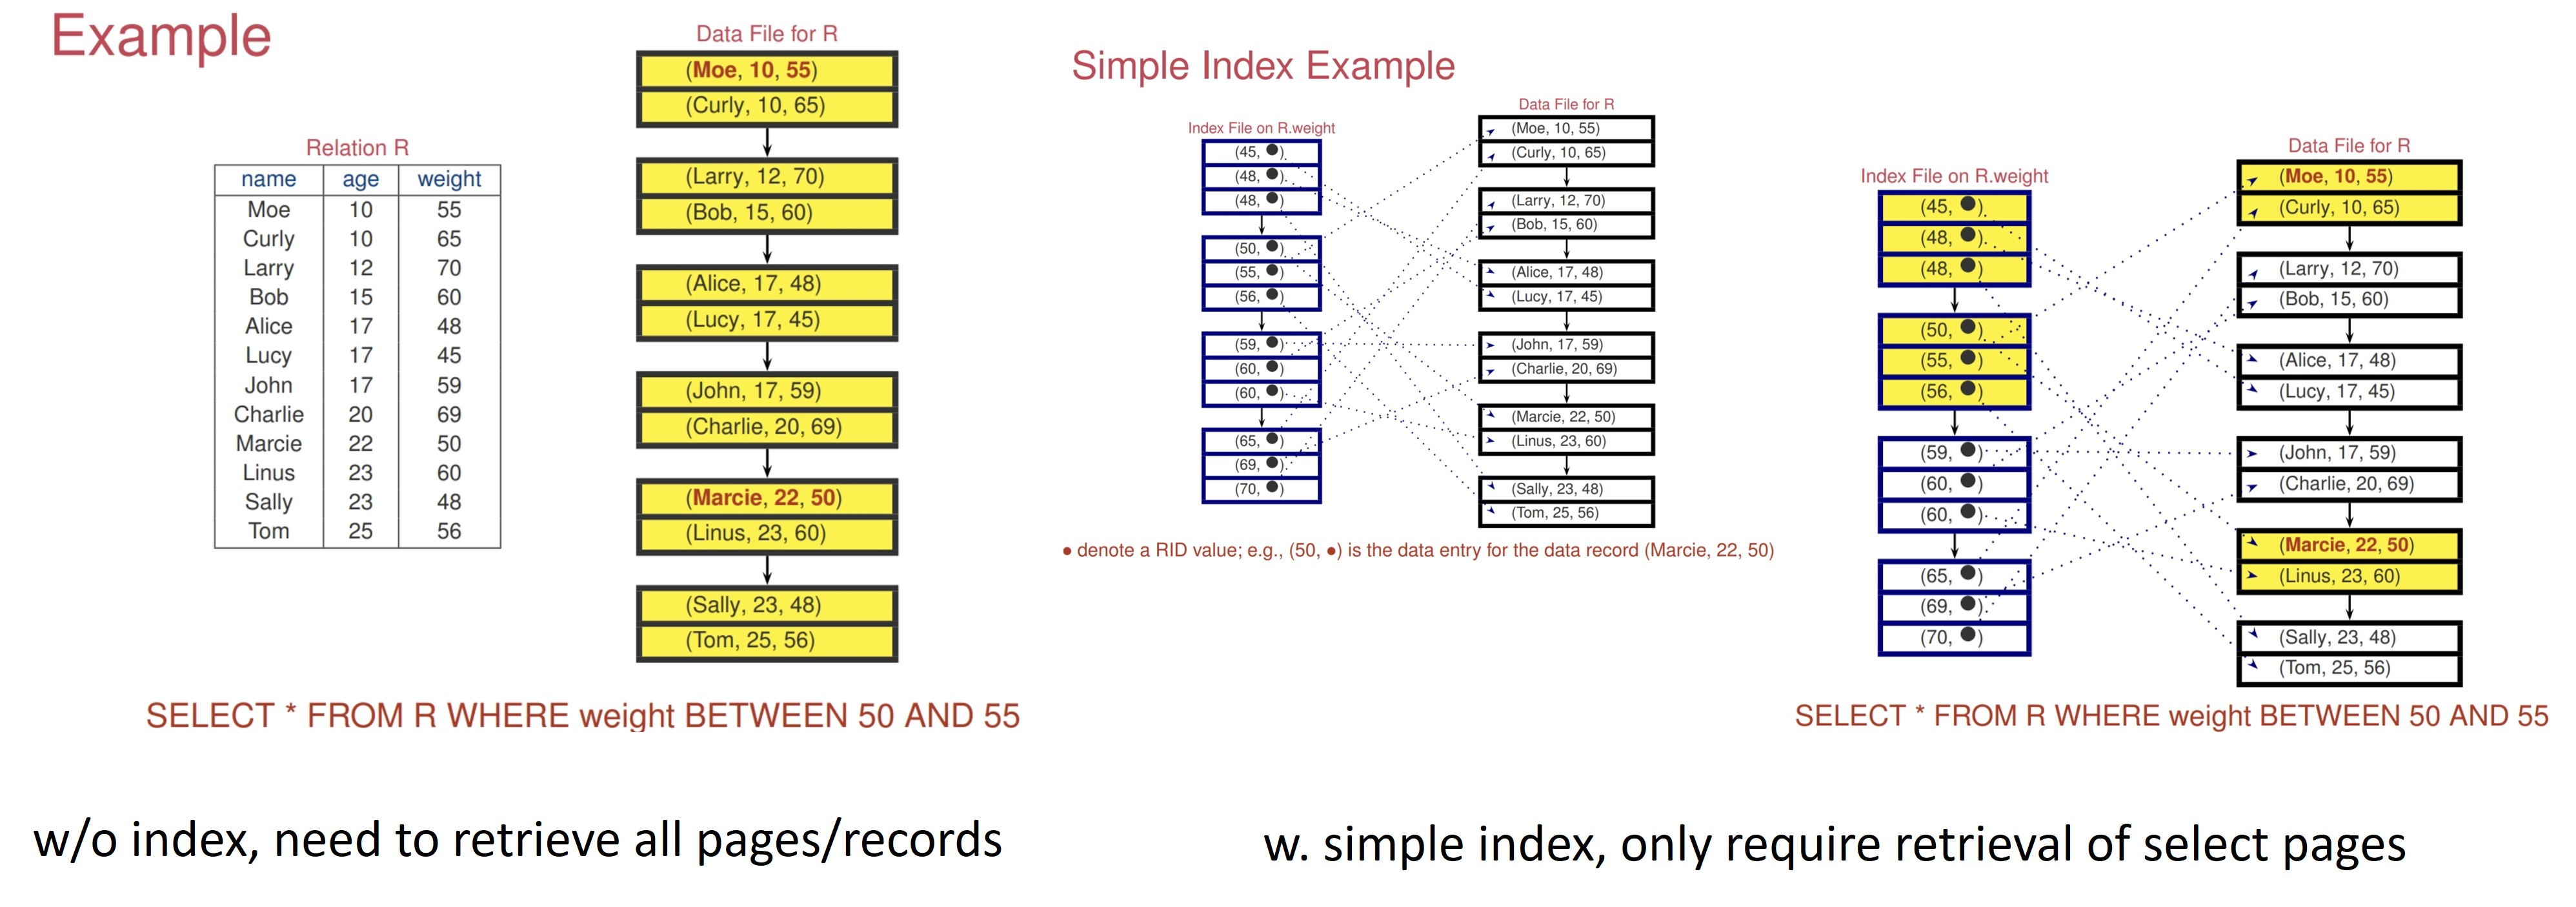
\includegraphics[width = 1\linewidth]{simpleIndex}}

\subsection{Index Types}
Two main types of indexes
\begin{itemize}
\item \textbf{Tree-based Index}: Based on sorting of search key values (E.g. ISAM, $B^+$-tree)
\item \textbf{Hash-based Index}: Data entries accessed using hashing function (E.g. static/ extendible / linear hashing)
\item Considerations when choosing an index: 
	\begin{itemize}
	\item Search Performance \\ 
	(Equality search: $k=v$, use hash-based.) (Range search, use tree)
	\item Storage overhead
	\item Update performance
	\end{itemize}
\end{itemize}

\subsection{Tree-basd Indexing: $B^+$-Tree }
$B^+$ tree is a dynamic structure that adjusts to changes in the file gracefully, most widely used index structure as it adjusts well to changes and supports both equality and range queries.
\begin{itemize}
\item \textbf{Balanced tree}: Operations (insert, delete) on tree keep it balanced.
\item \textbf{Internal nodes} direct the search.
\item \textbf{Leaf nodes} contain the data entries. Leaf pages linked using page pointers for easy traversal of sequence of leaf pages in either direciton.
\item \textbf{Value $d$} is parameter of $B^+$-tree, called order of the tree, is a measure of capacity of a tree node. Each node contains $m$ entries, where $d \leq m \leq 2d$, except root node, where $1 \leq m \leq 2d$
\end{itemize}


\subsection{$B^+$-tree Index}
\centerline{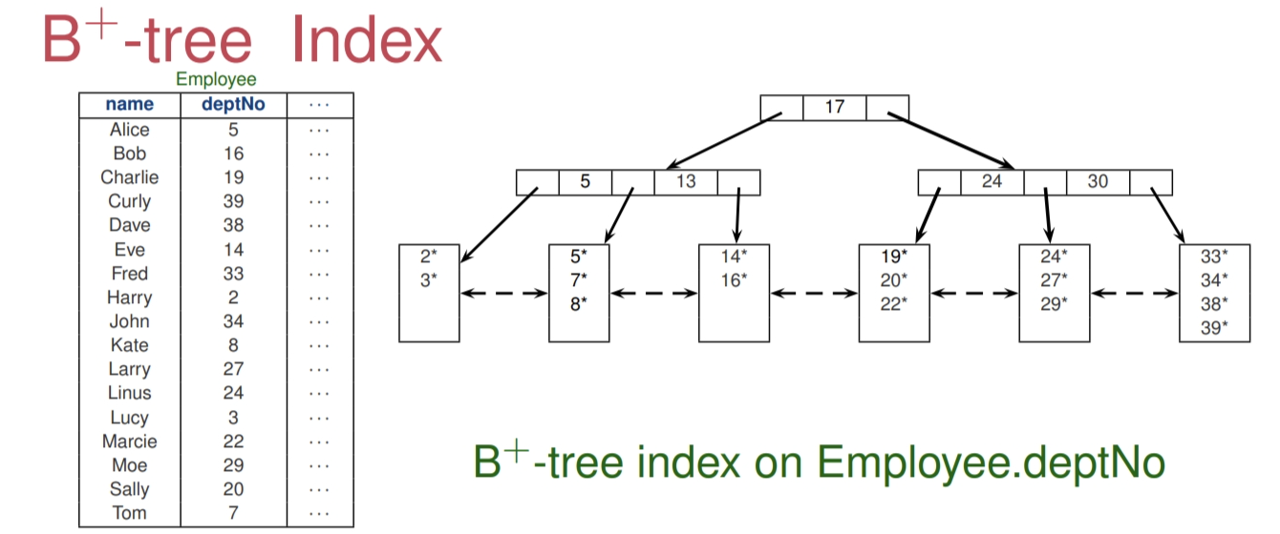
\includegraphics[width = 1\linewidth]{B+TreeIndex}}
\begin{itemize}
\item Each node is either a \textbf{leaf node} (bottom-most level) or an internal node. 
\item Top-most internal node is the \textbf{root node} located at \textbf{level 0}.
\item \textbf{Height of Tree} = number of level of internal nodes. (Leaf nodes are at level $h$ where $h$ = height of tree.
\item Nodes at same level are \textbf{sibling nodes} if they have the same parent node.
\item \textbf{Leaf Nodes}:
	\begin{itemize}
	\item Leaf nodes store sorted data entries.
	\item $k*$ denote data entry of form (k, RID), where k = search key value of corresponding data record, RID = RID of data record.
	\item Lead nodes are doubly-linked to adjacent nodes.
	\end{itemize}
\item \textbf{Internal Nodes}:
	\begin{itemize}
	\item Internal nodes store index entries of the form (p: pointer, k: separator)\\
	 $(p_0, k_1, p_1, k_2, p_2, ..., p_n)$
	\item $k_1 < k_2 < ... < K_n$
	\item Each $(k_i, p_i)$ is an \textbf{index entry}, $k_i$ serves as \textbf{separator} between node contents pointed to by $p_{i-1}$ \& $p_i$
	\item $p_i$ = disk page address (root node of an index subtree $T_i$)
	\end{itemize}
\end{itemize}

\null \null
\columnbreak

\subsection{$B^+$-tree Index Properties}
\centerline{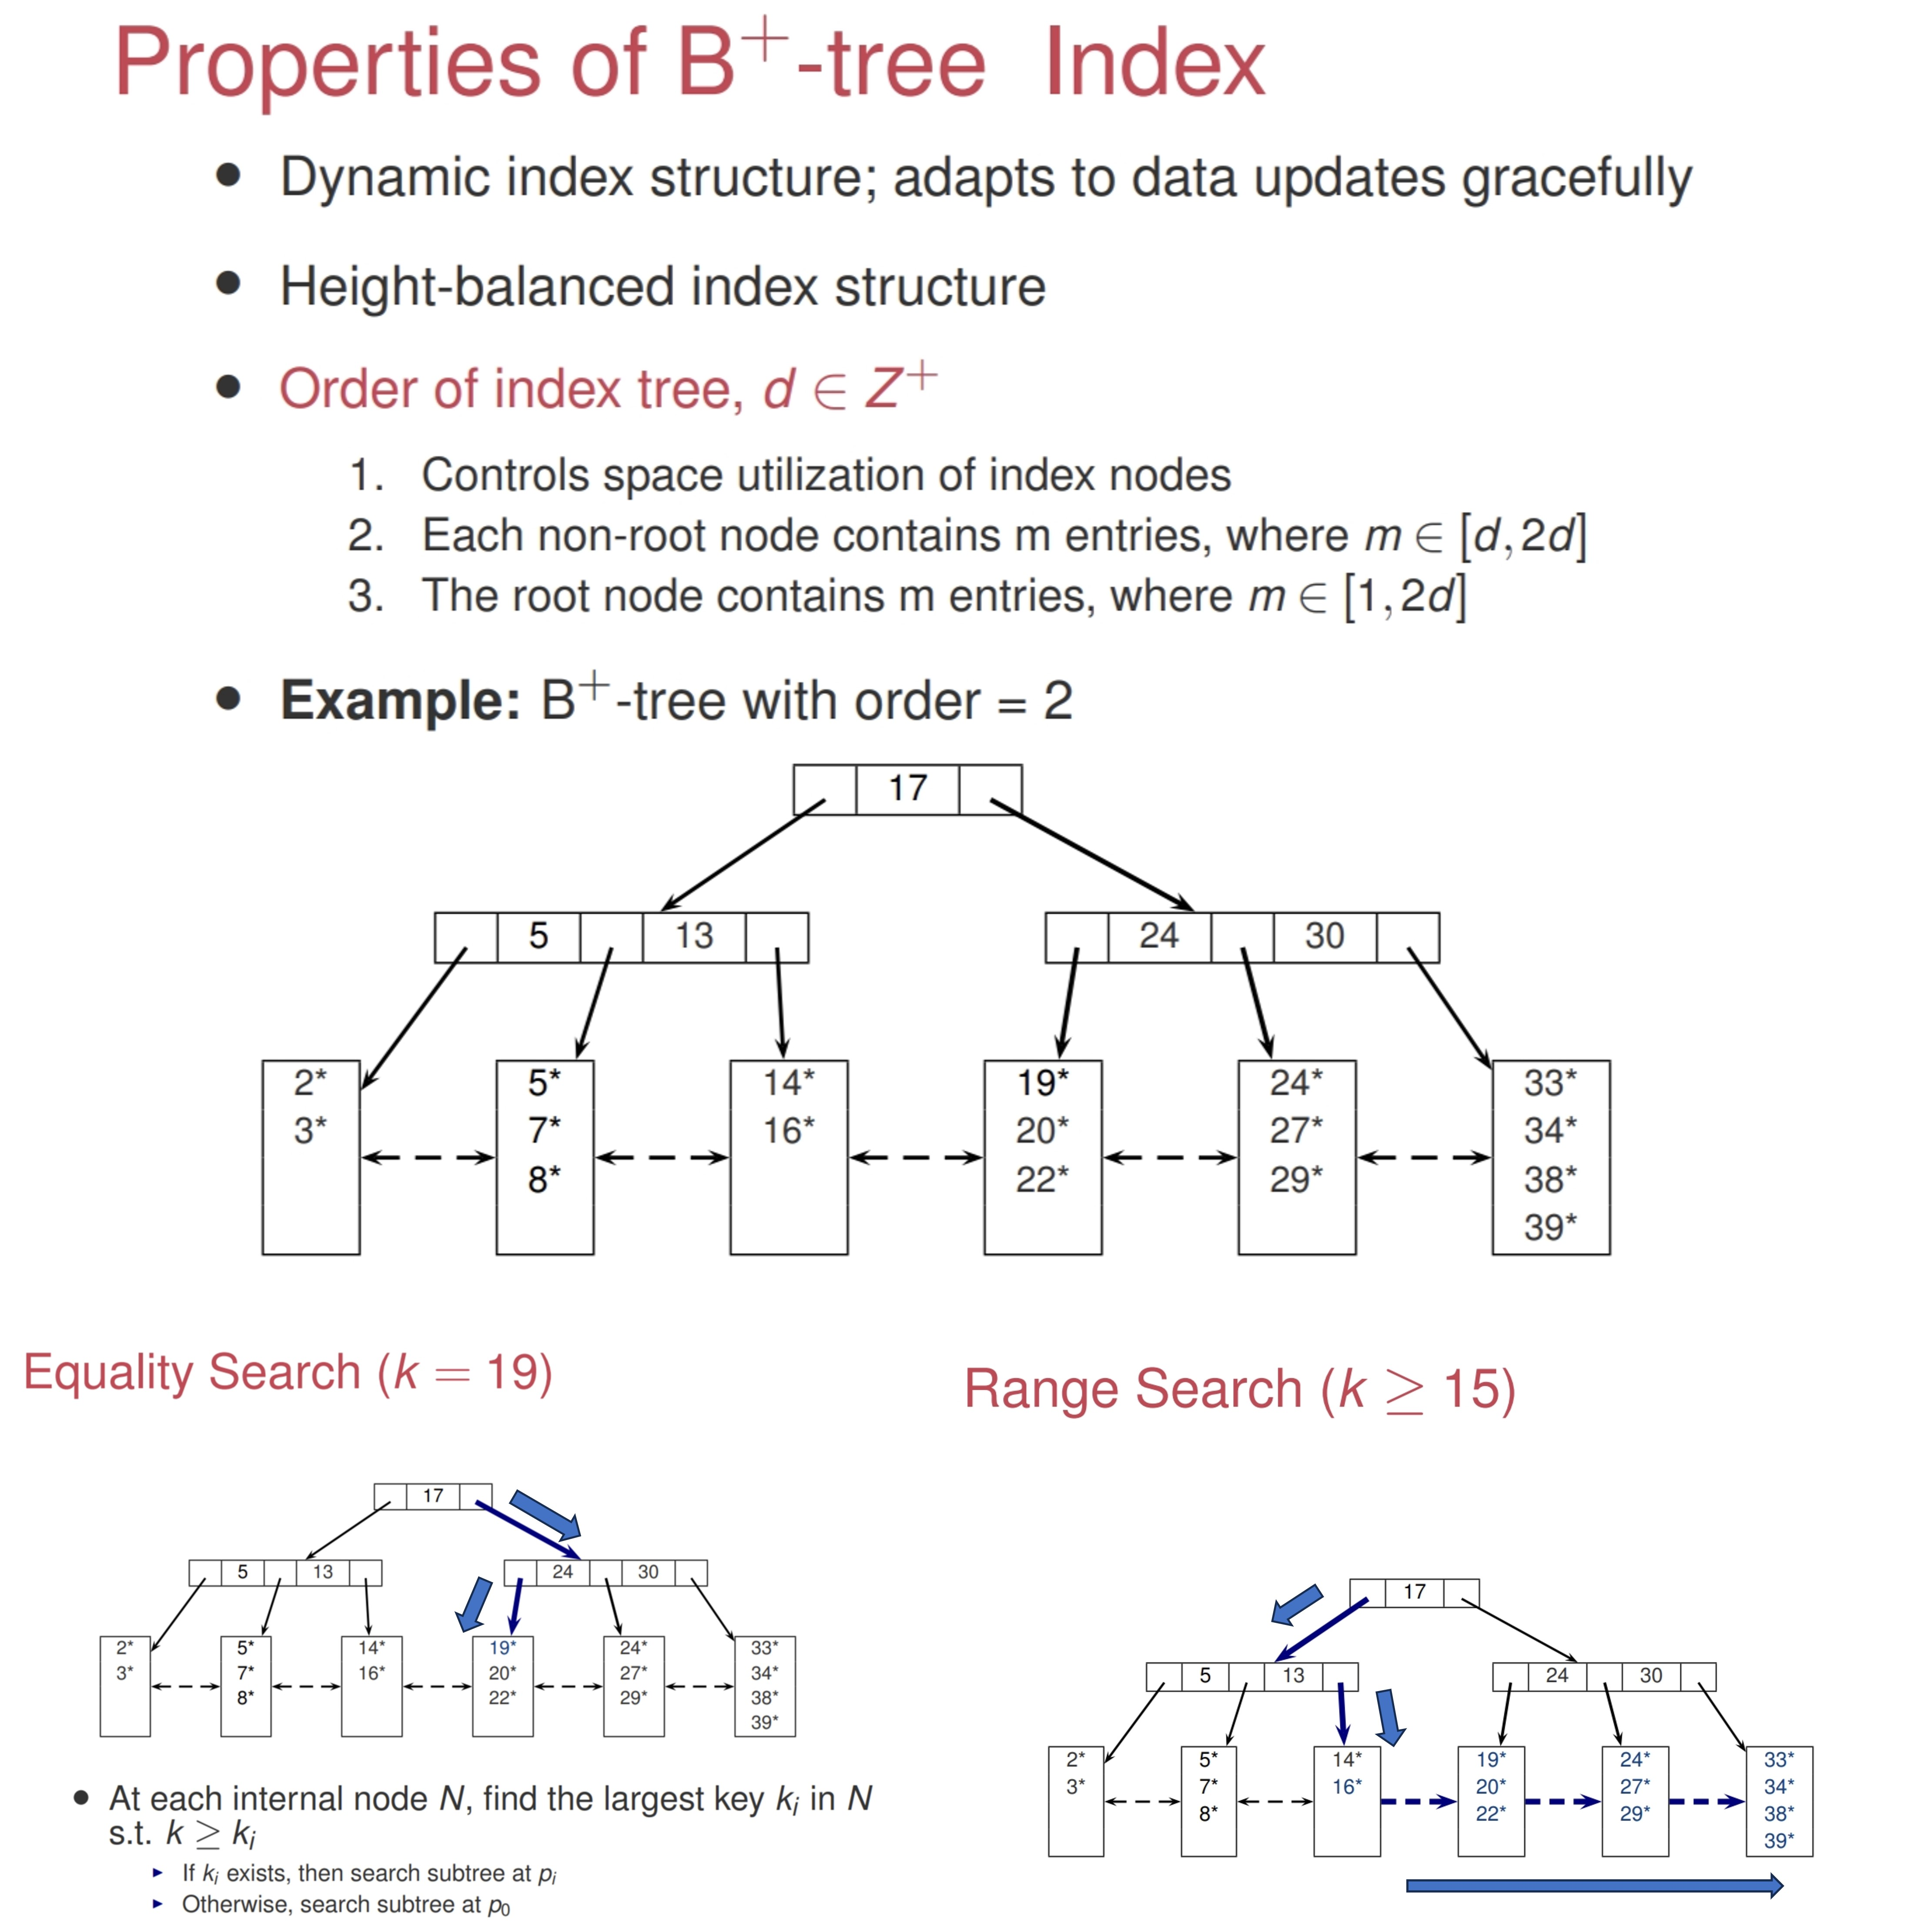
\includegraphics[width = 1\linewidth]{Bproperties}}

\subsubsection{Formats of Data Entries in B-Tree}
\begin{itemize}
\item \textbf{Format 1}: k* is actual \textit{data record} (with search key value $k$)
\item \textbf{Format 2}: k* is of form \textit{(k, rid)}, where rid is record identifier of record with search key value $k$.
\item \textbf{Format 3}: k* is of form \textit{(k, rid-list)}, where rid-list is list of record identifiers of data records with search key value $k$.
\item Note, examples assume Format 2.
\end{itemize}
\centerline{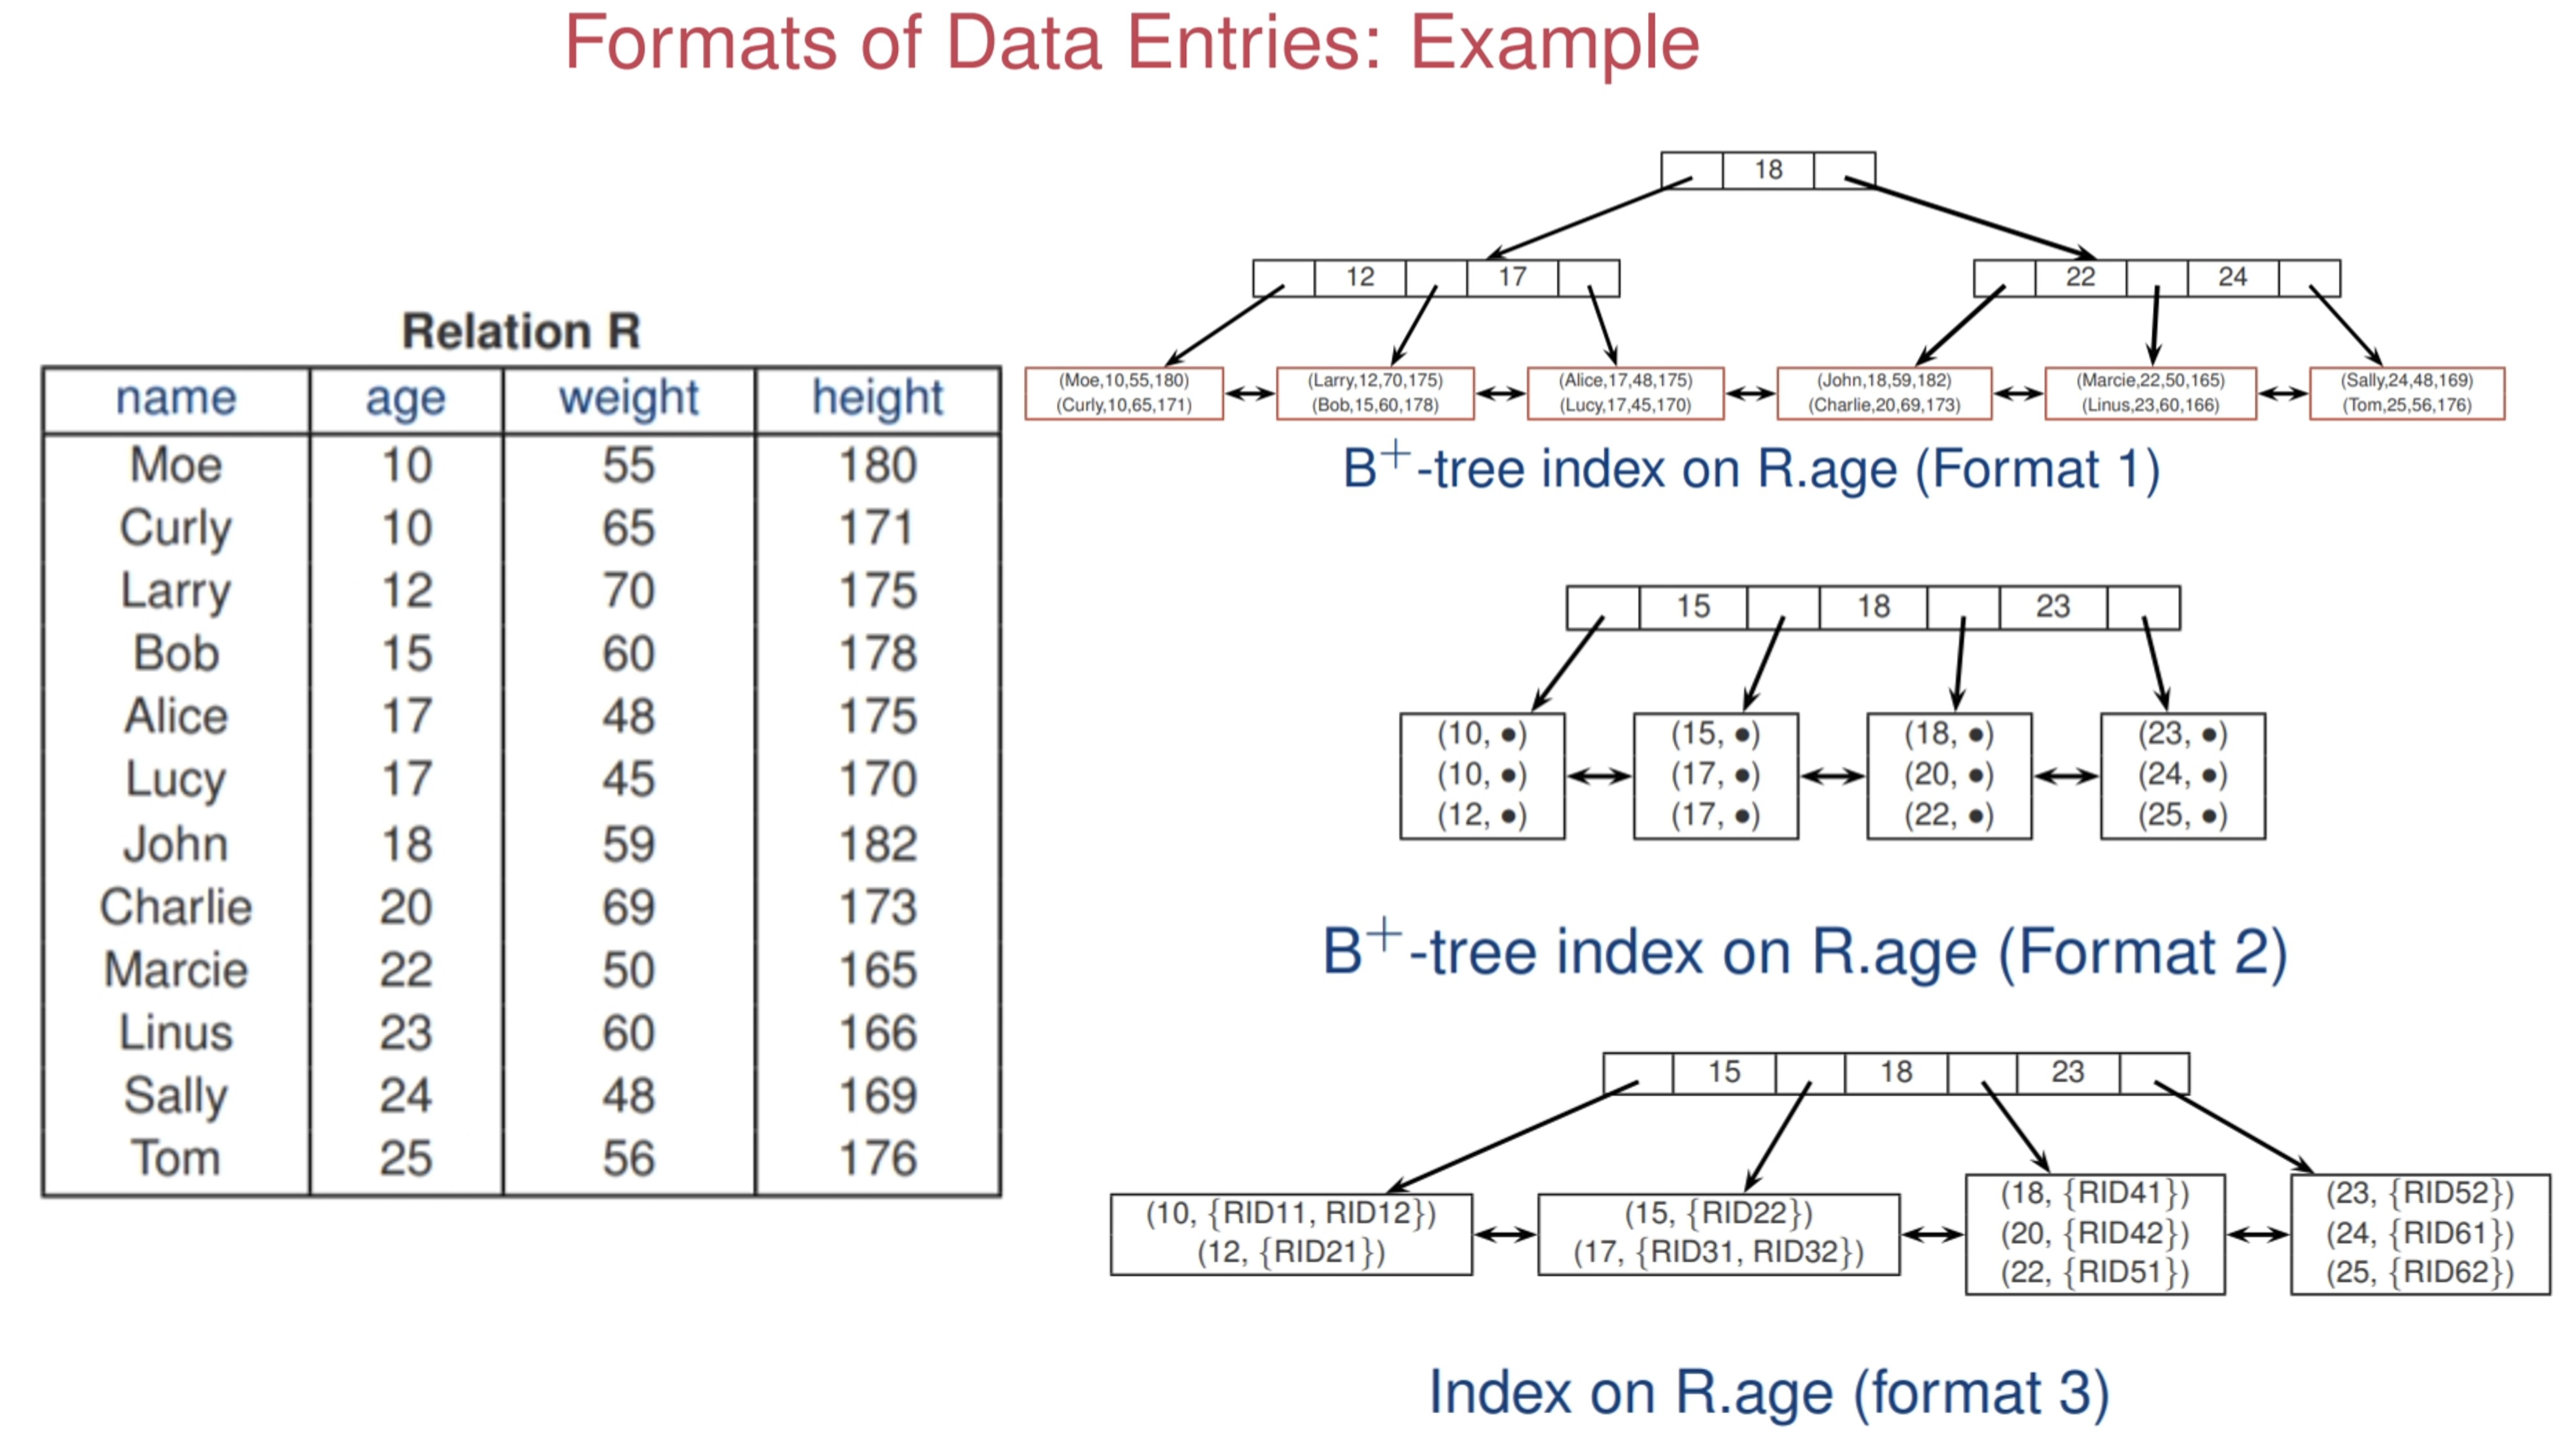
\includegraphics[width = 0.9\linewidth]{dataFormat}}

\subsubsection{$B^+$-tree Search Algorithms }
\begin{itemize}
\item Search algorithm finds the leaf node a given data entry belongs to.
\item We assume no duplicates, no data entries same key value. Note in practice, duplicates arise whenever search key does not contain candidate key, must be dealt with.
\end{itemize}
\centerline{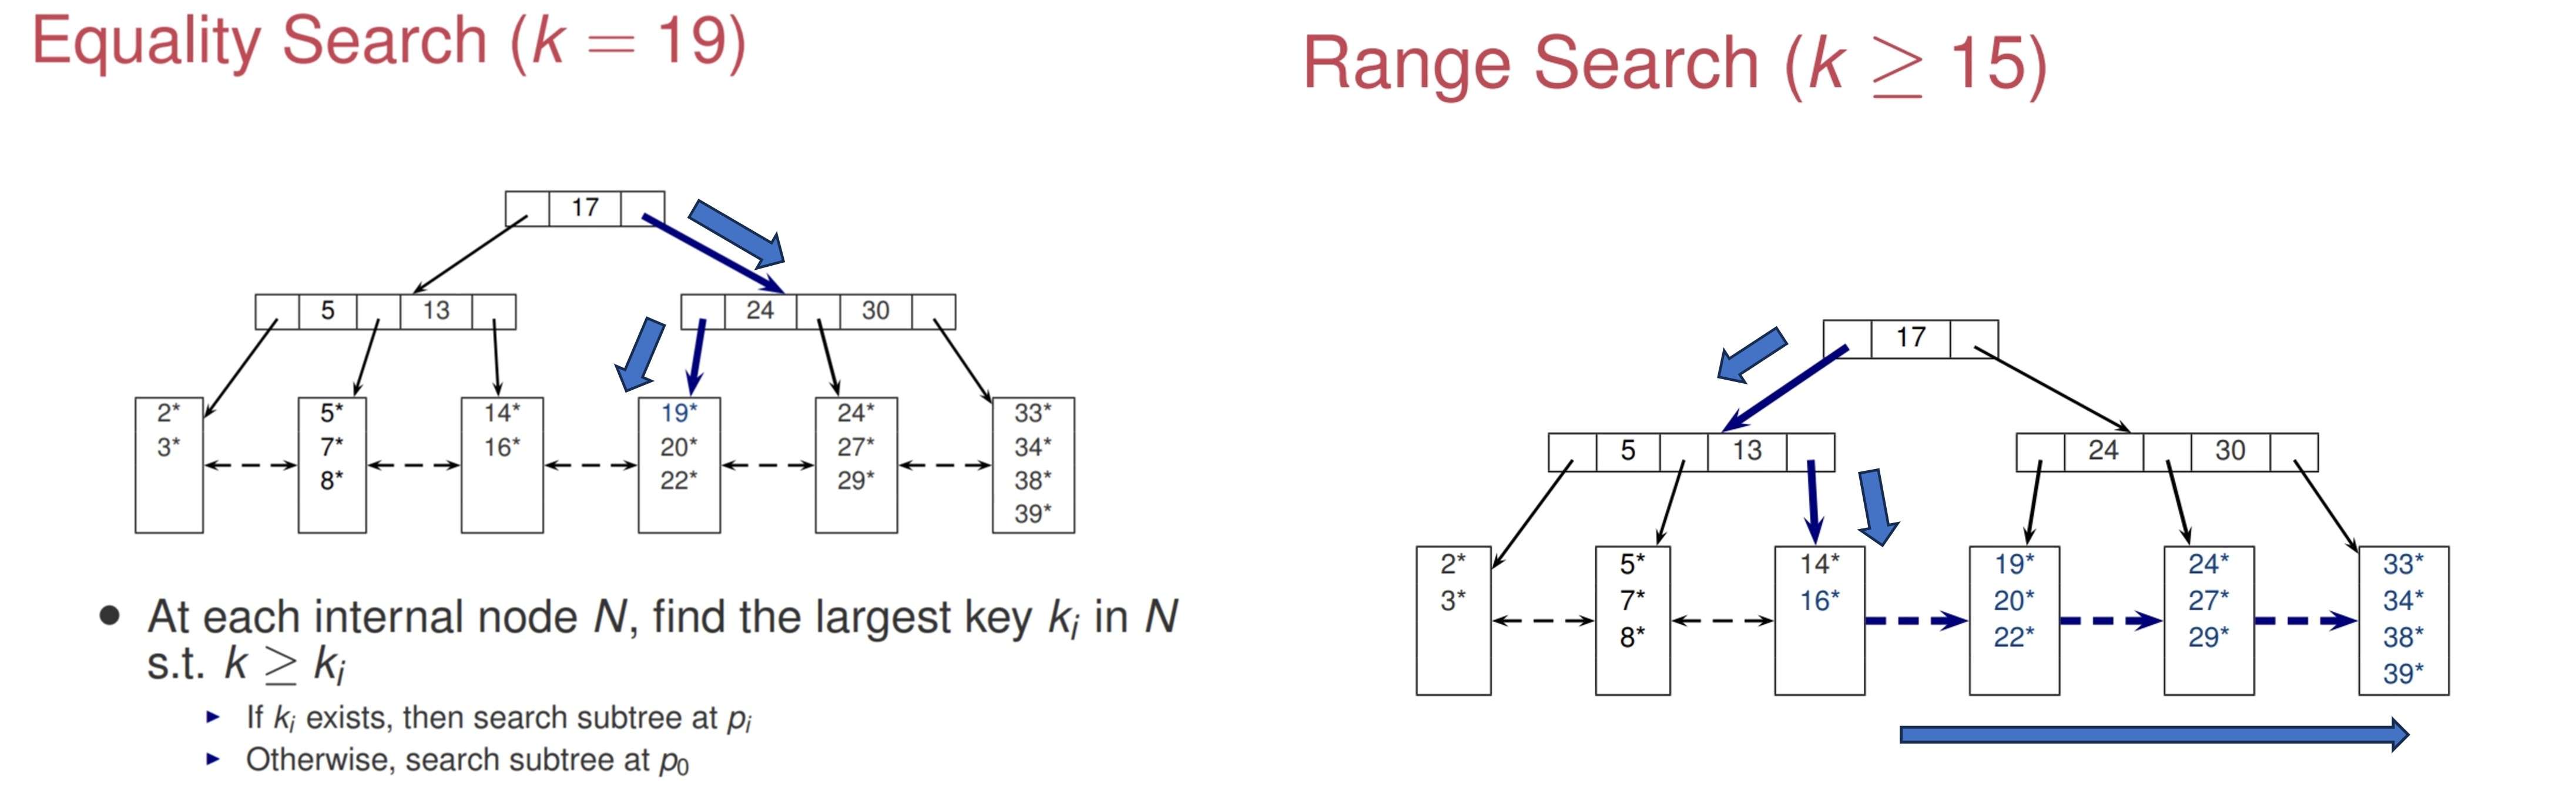
\includegraphics[width = 1\linewidth]{Bsearch}}

\columnbreak

\subsection{$B^+$-Tree Insertion}
\begin{itemize}
\item \textbf{Algorithm for insertion} takes an entry, finds the leaf node where it belongs, and inserts it there.
\item Occasionally, a \textbf{node is full and must be split}. (More than $2d$ entries) When node is split, entry pointing to the node created by the split must be inserted into the parent. 
\item If the (old) root is split, a new root node is created and height of tree increases by 1. 
\end{itemize}


\subsubsection{Splitting of overflowed node}
\begin{itemize}
\item Split overflowed leaf node by distributing $d + 1$ entries to new leaf node.
\item Create a new entry index using smallest key in leaf node.
\item Insert new index entry into parent node of overflowed node.
\end{itemize}
\centerline{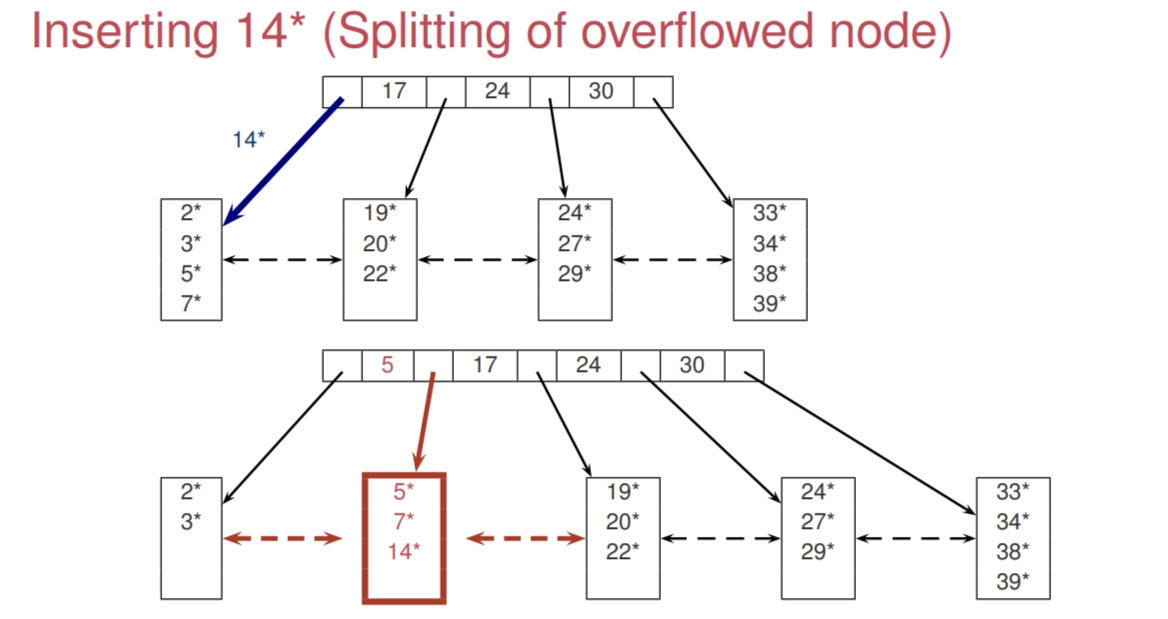
\includegraphics[width = 0.7\linewidth]{Binsertion}}
\begin{itemize}
\item Sometimes, \textbf{node split is propagated upwards} to ancestor internal nodes.
\item When splitting an \textbf{internal node}, the middle key is pushed to parent node.
\end{itemize}
\centerline{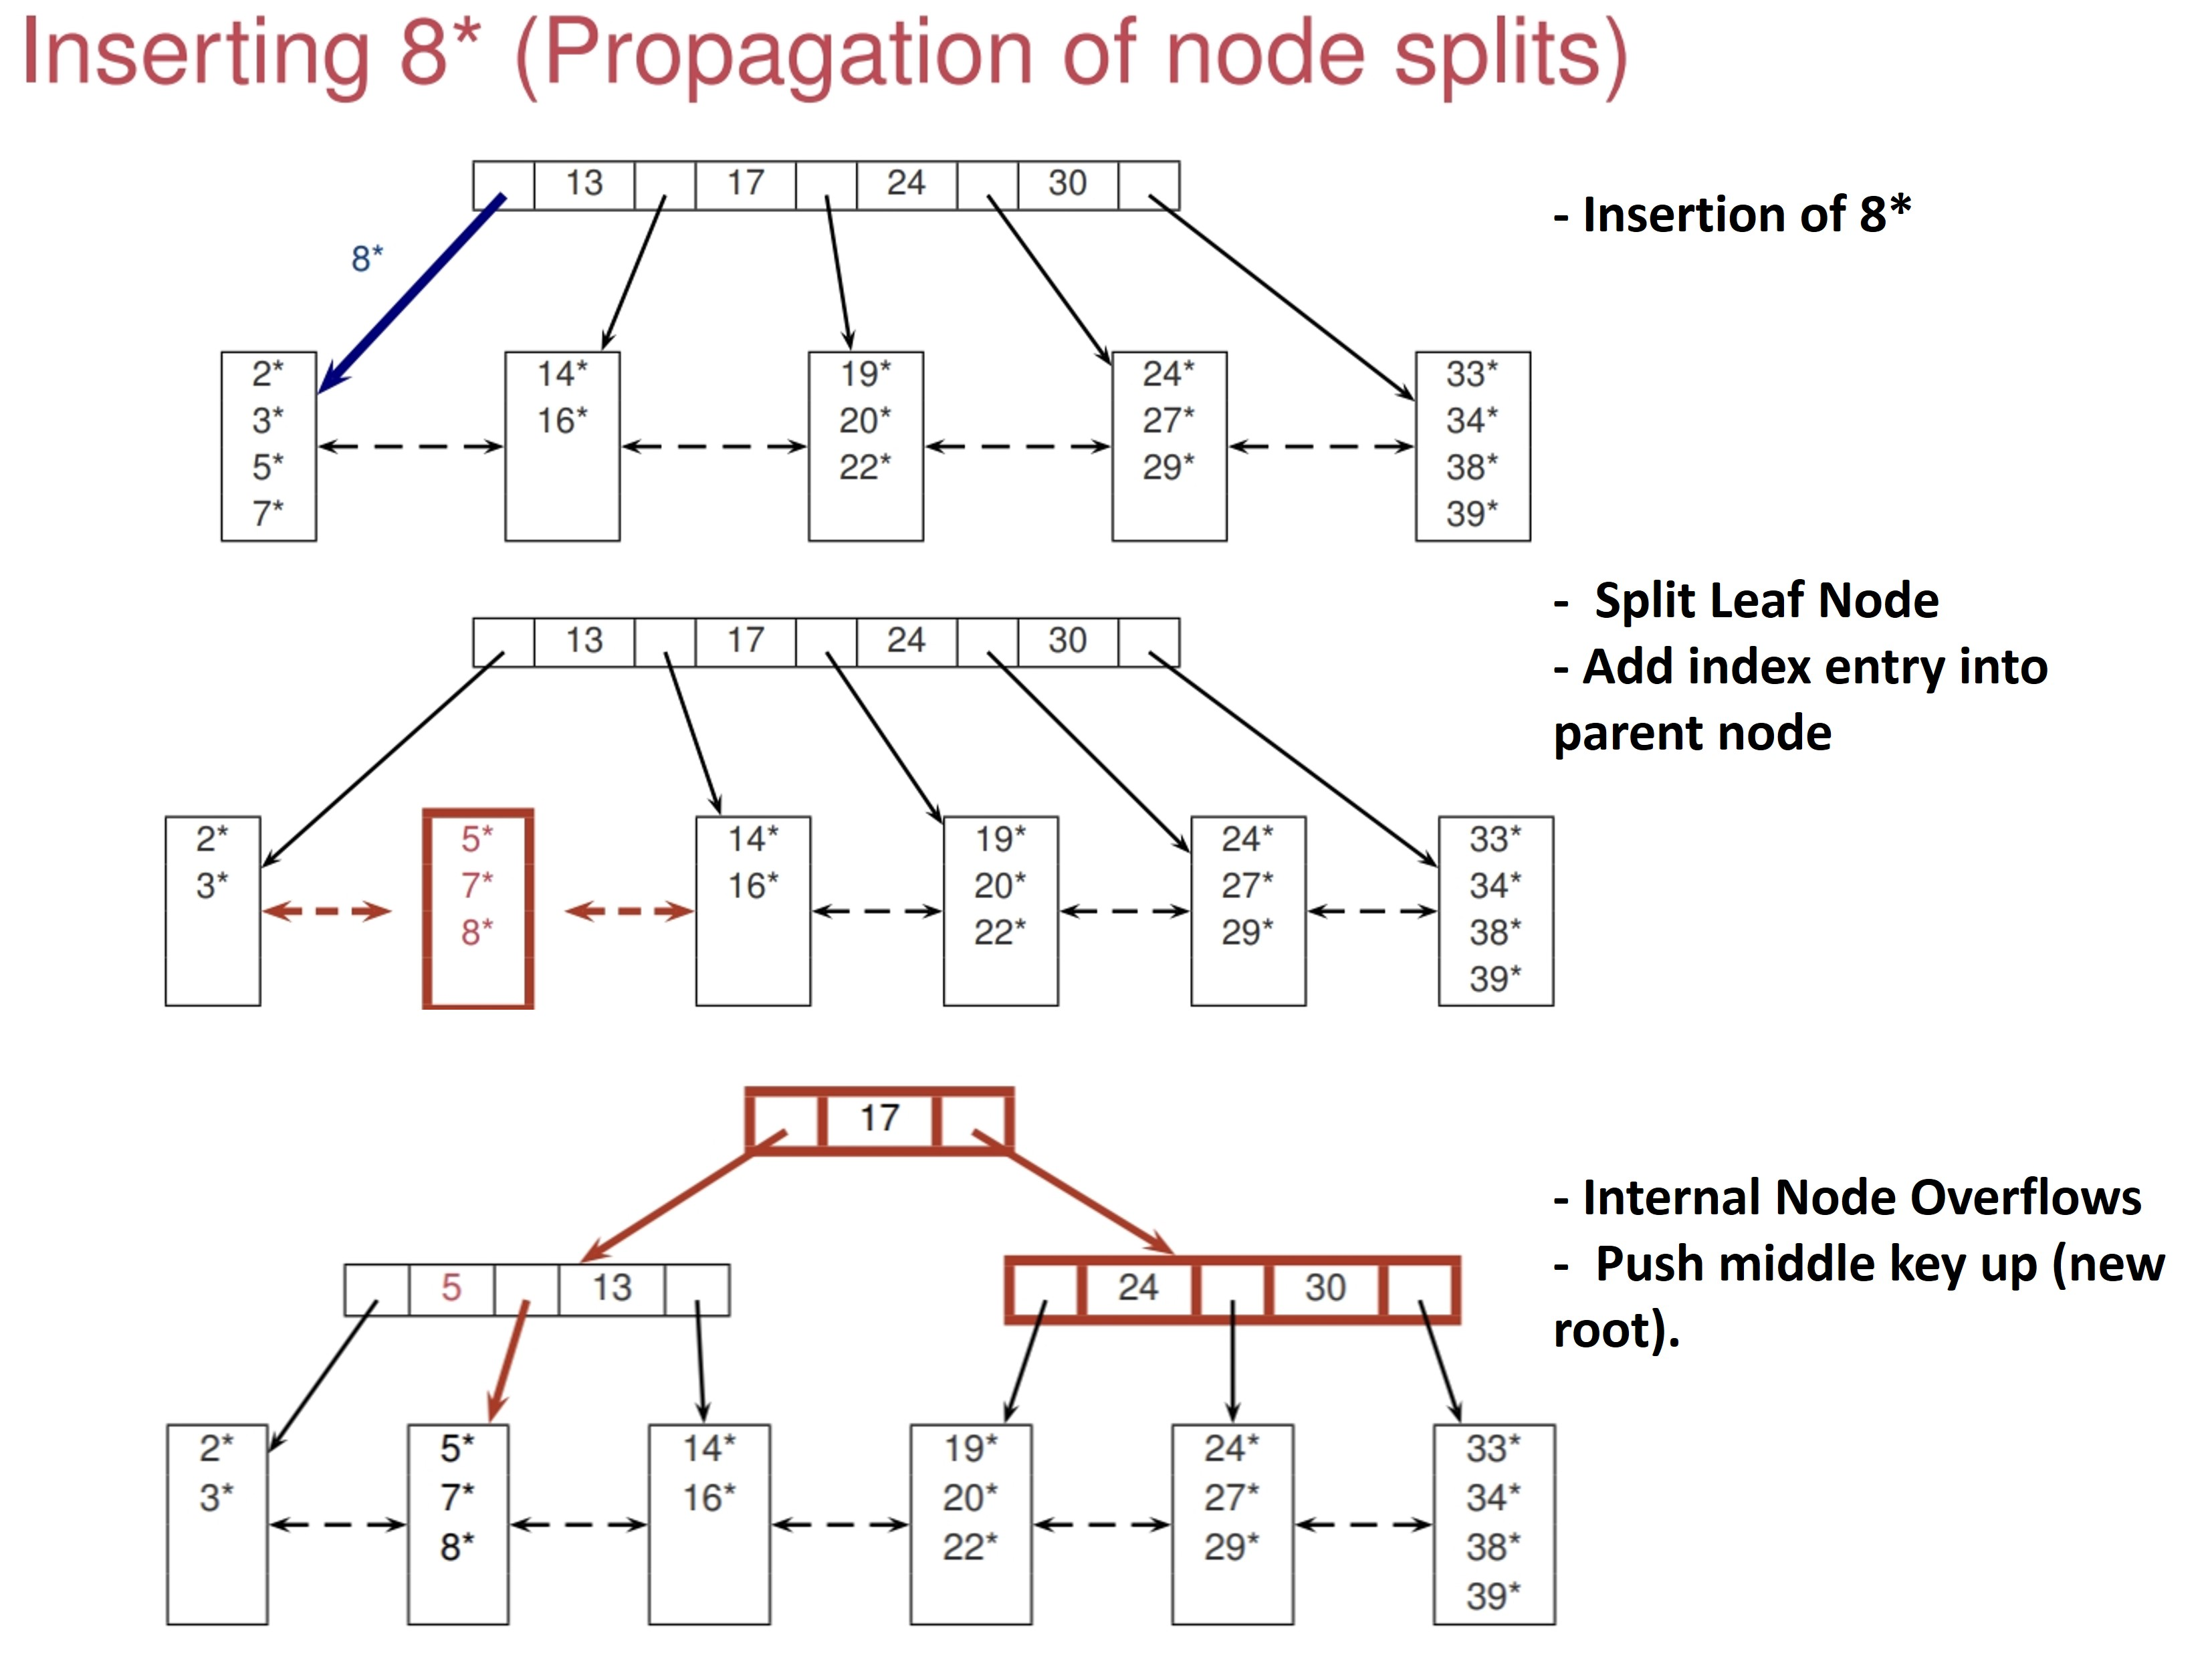
\includegraphics[width = 0.95\linewidth]{Binsertion2}}
\centerline{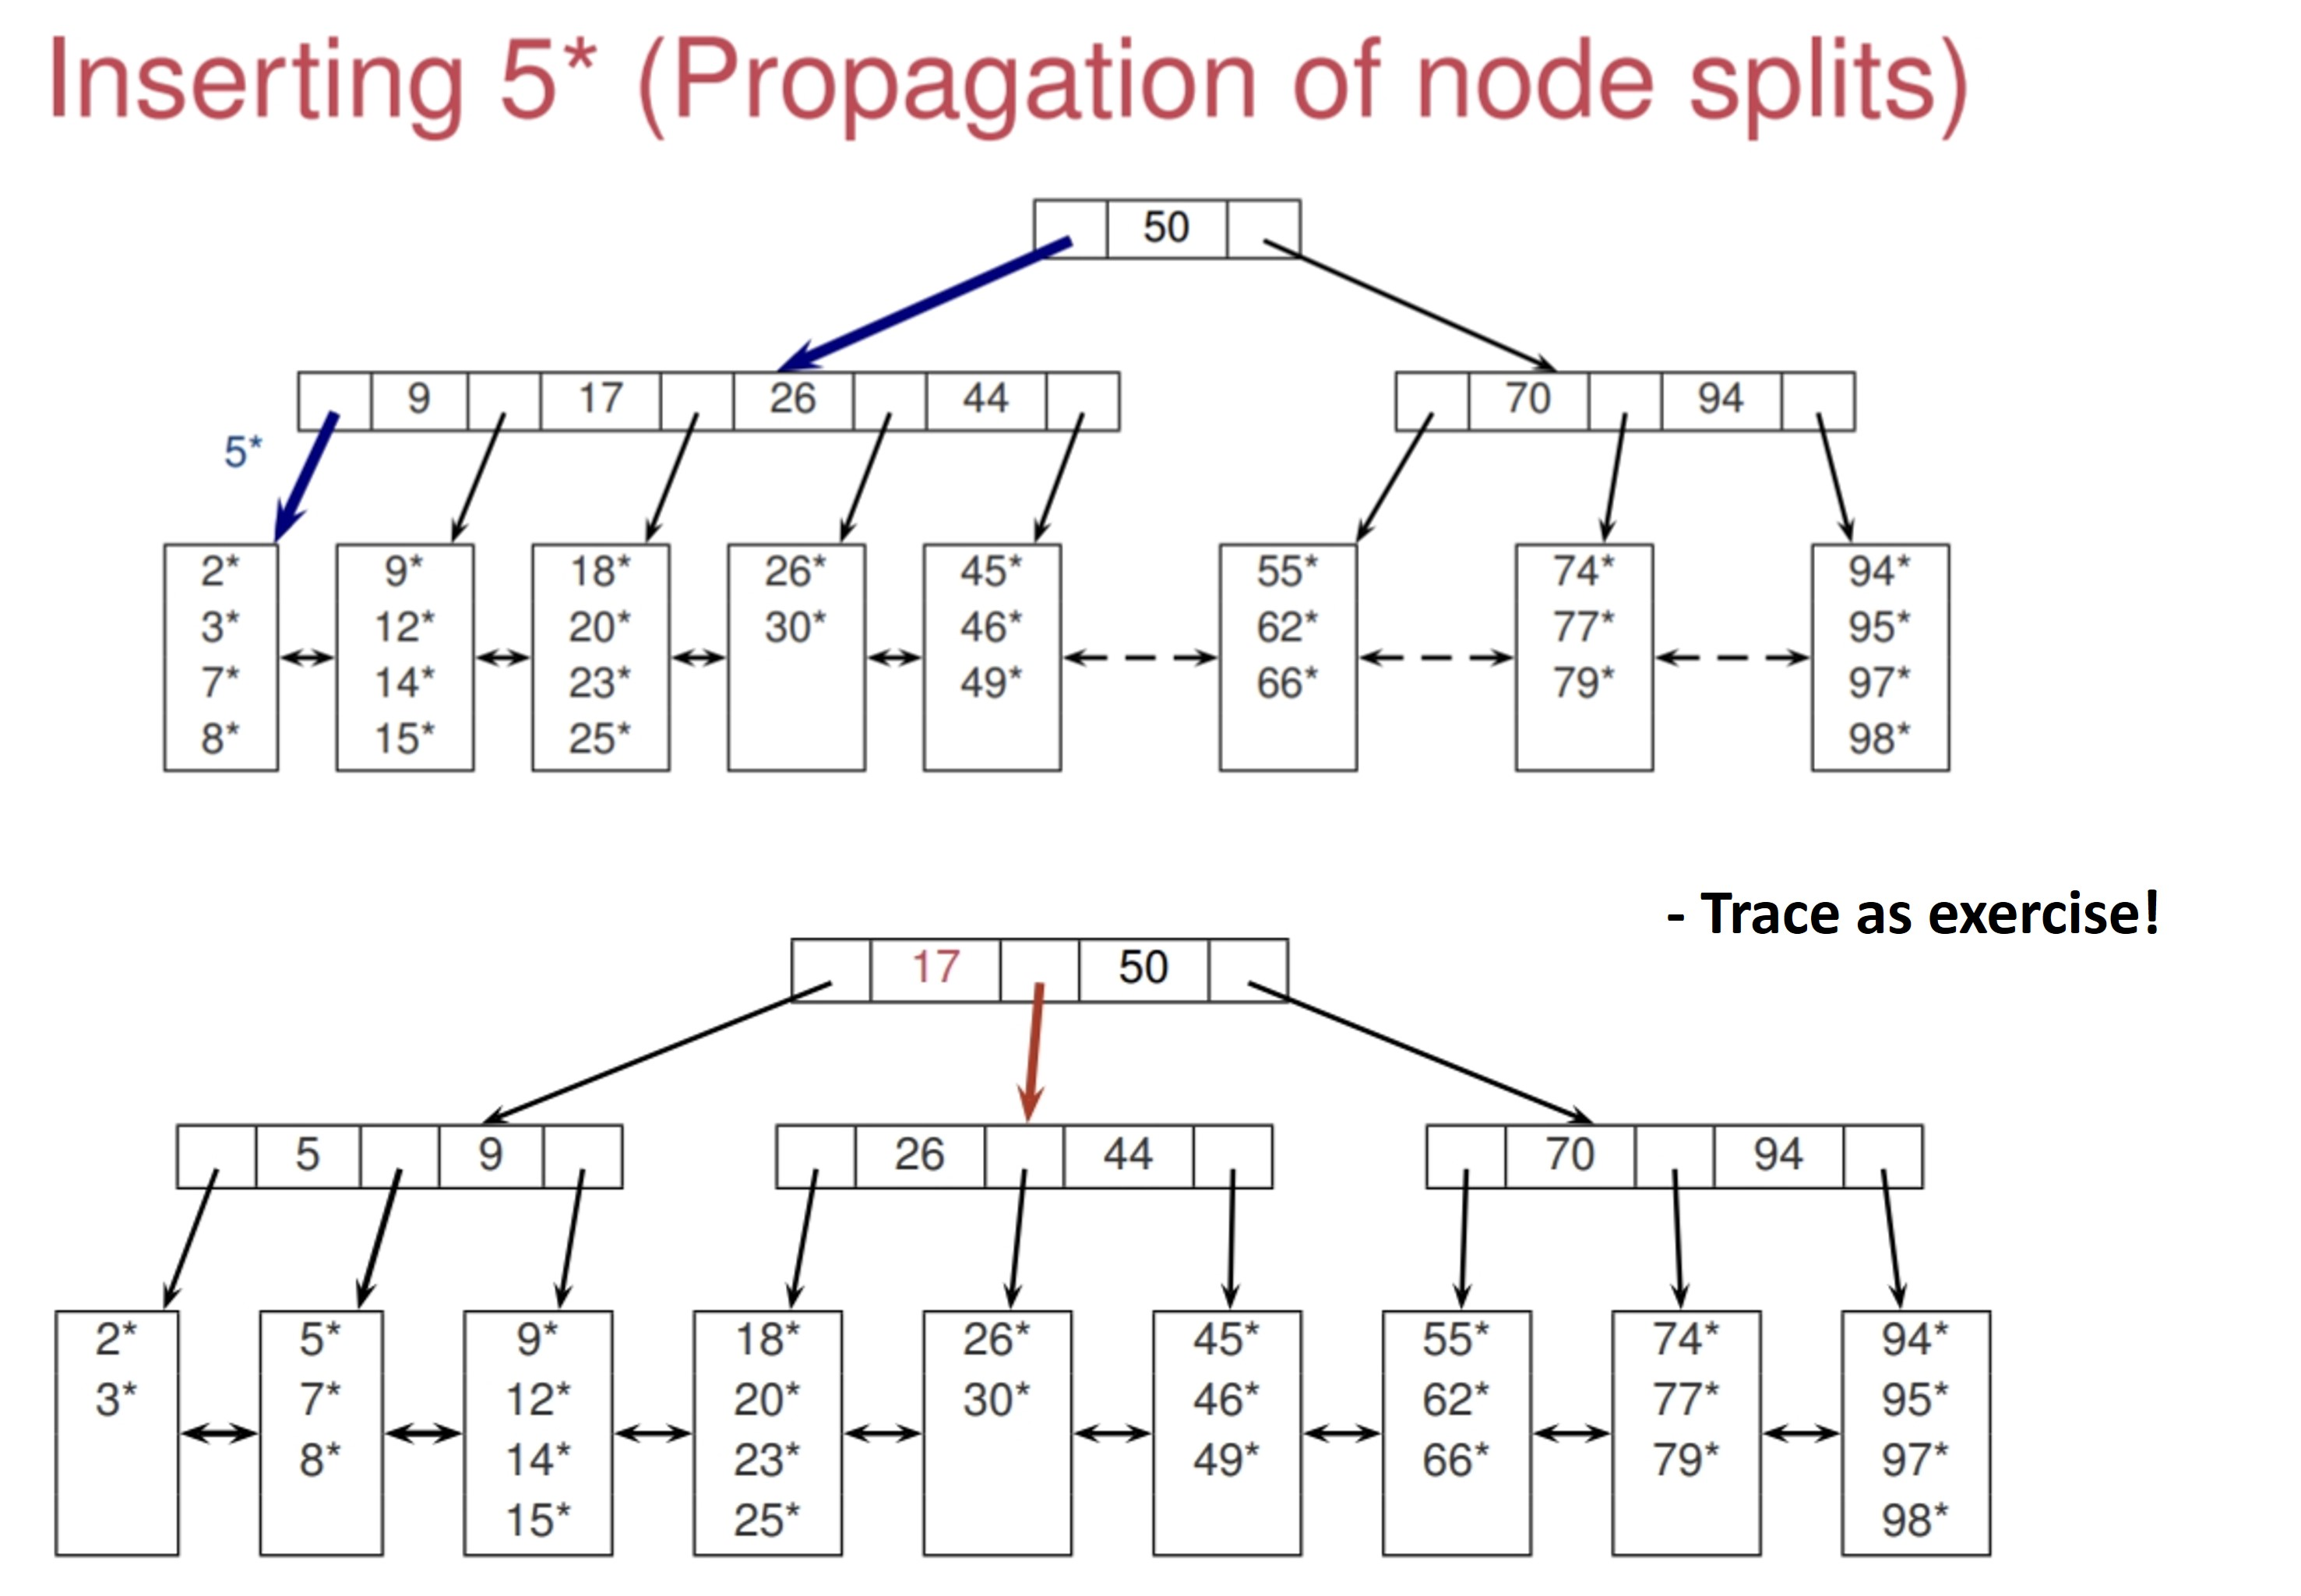
\includegraphics[width = 0.8\linewidth]{Binsertion3}}

\subsubsection{Redistributing of data entries in Overflow}
\begin{itemize}
\item A node split can sometimes be avoided by distributing entries from overflowed node to a non-full adjacent sibling node.
\end{itemize}
\centerline{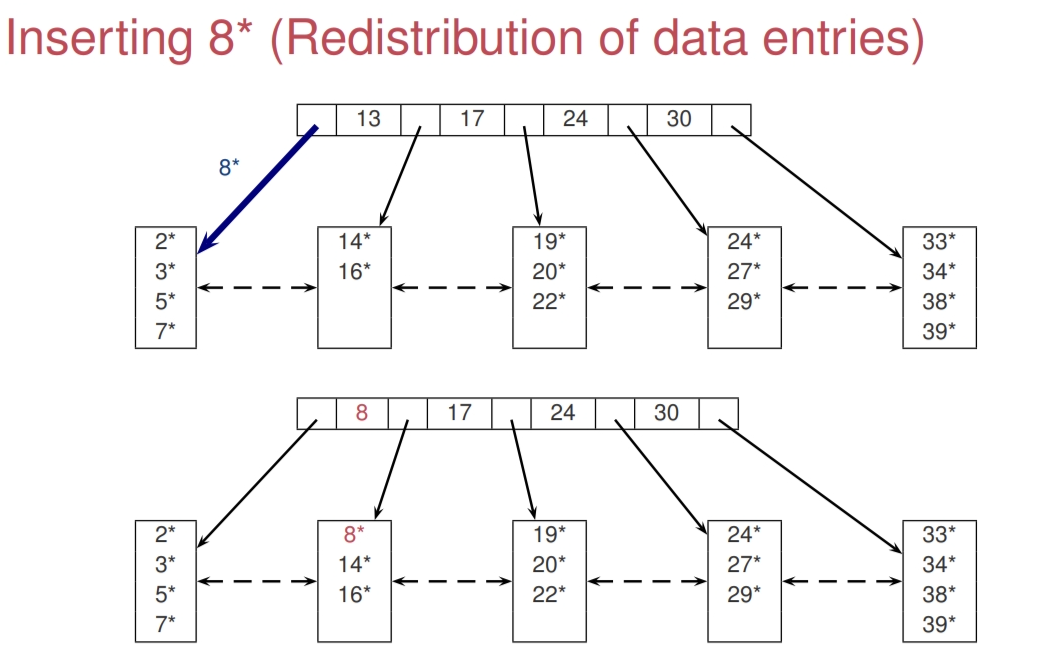
\includegraphics[width = 0.8\linewidth]{Binsertion4}}

\subsection{$B^+$-Tree Deletion}
\begin{itemize}
\item \textbf{Algorithm for deletion} takes an entry, finds leaf node it belongs to, and deletes it.
\item \textbf	{Underflowed node}: When node is at minimum occupancy before deletion, and goes below threshold, we must either \textbf{redistribute entries from adjacent sibling}, or \textbf{merge node with sibling} to maintain minimum occupancy.
\item \textbf{Merging}: Underflowed node needs to be merged if each of \textbf{adjacent} sibling nodes has exactly $d$ entries.
\end{itemize}
\centerline{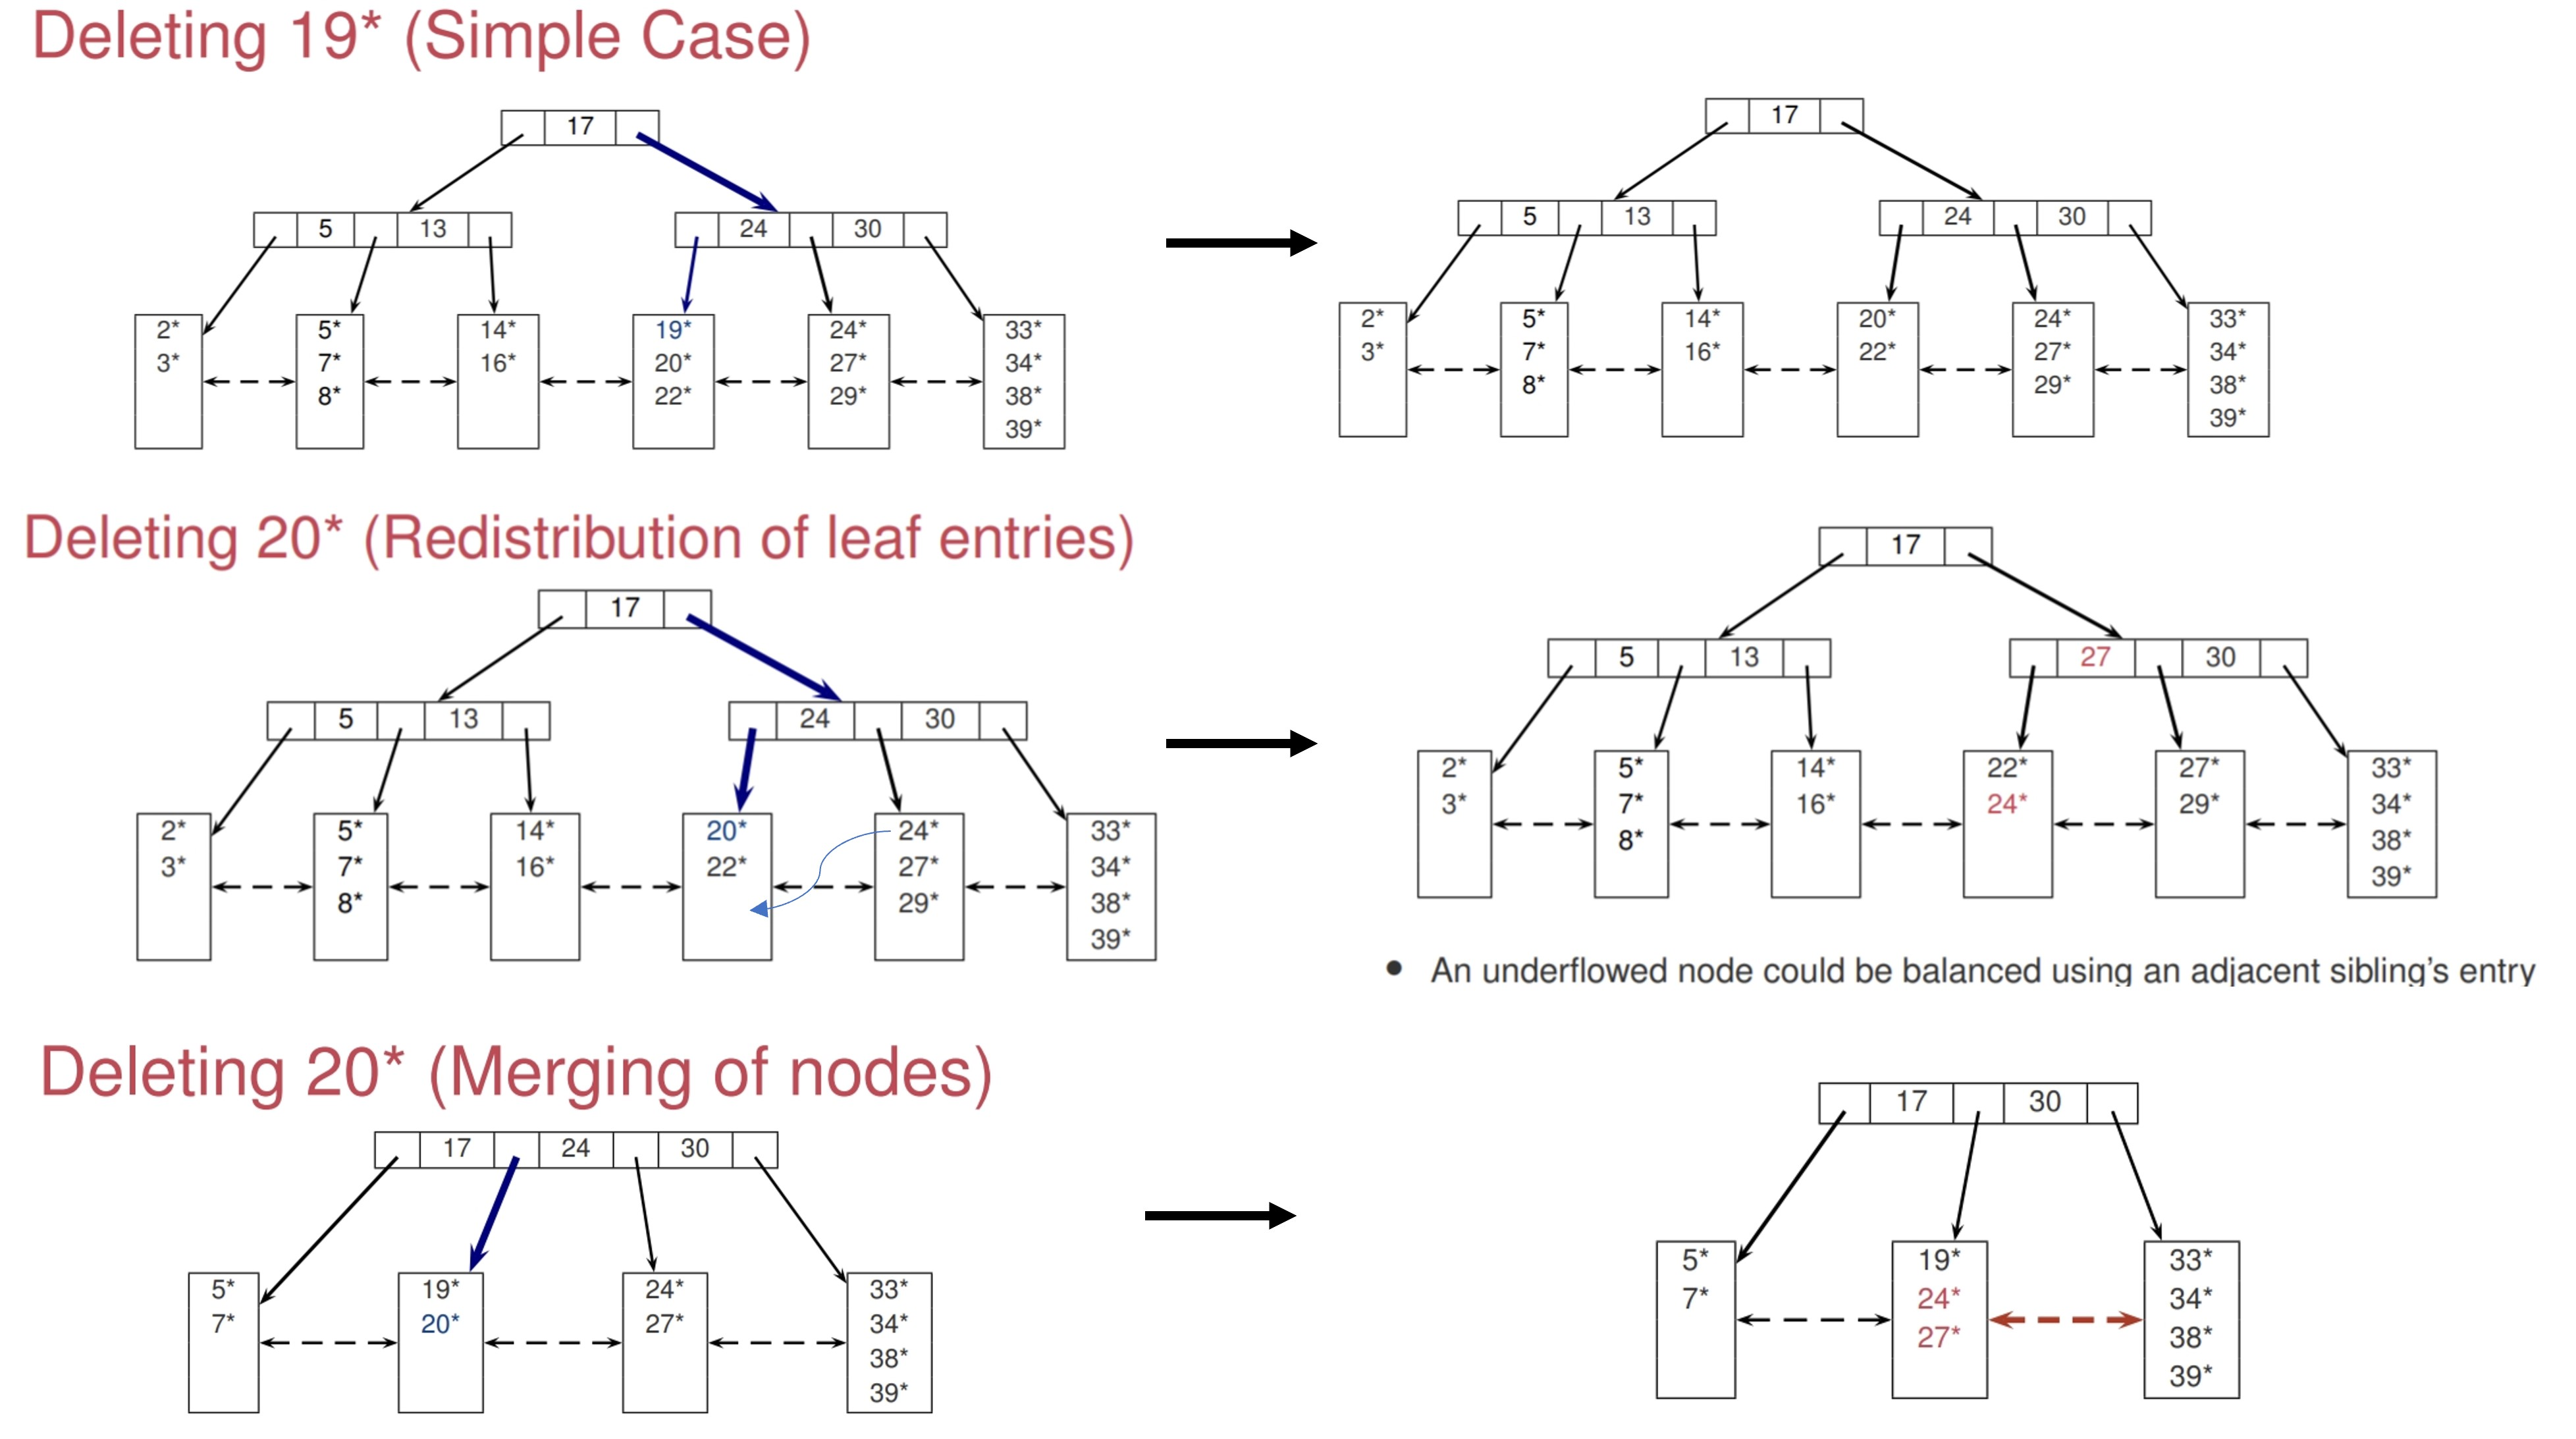
\includegraphics[width = 1\linewidth]{Bdeletion1}}
\begin{itemize}
\item  Node mergers may propagate upwards.
\end{itemize}
\centerline{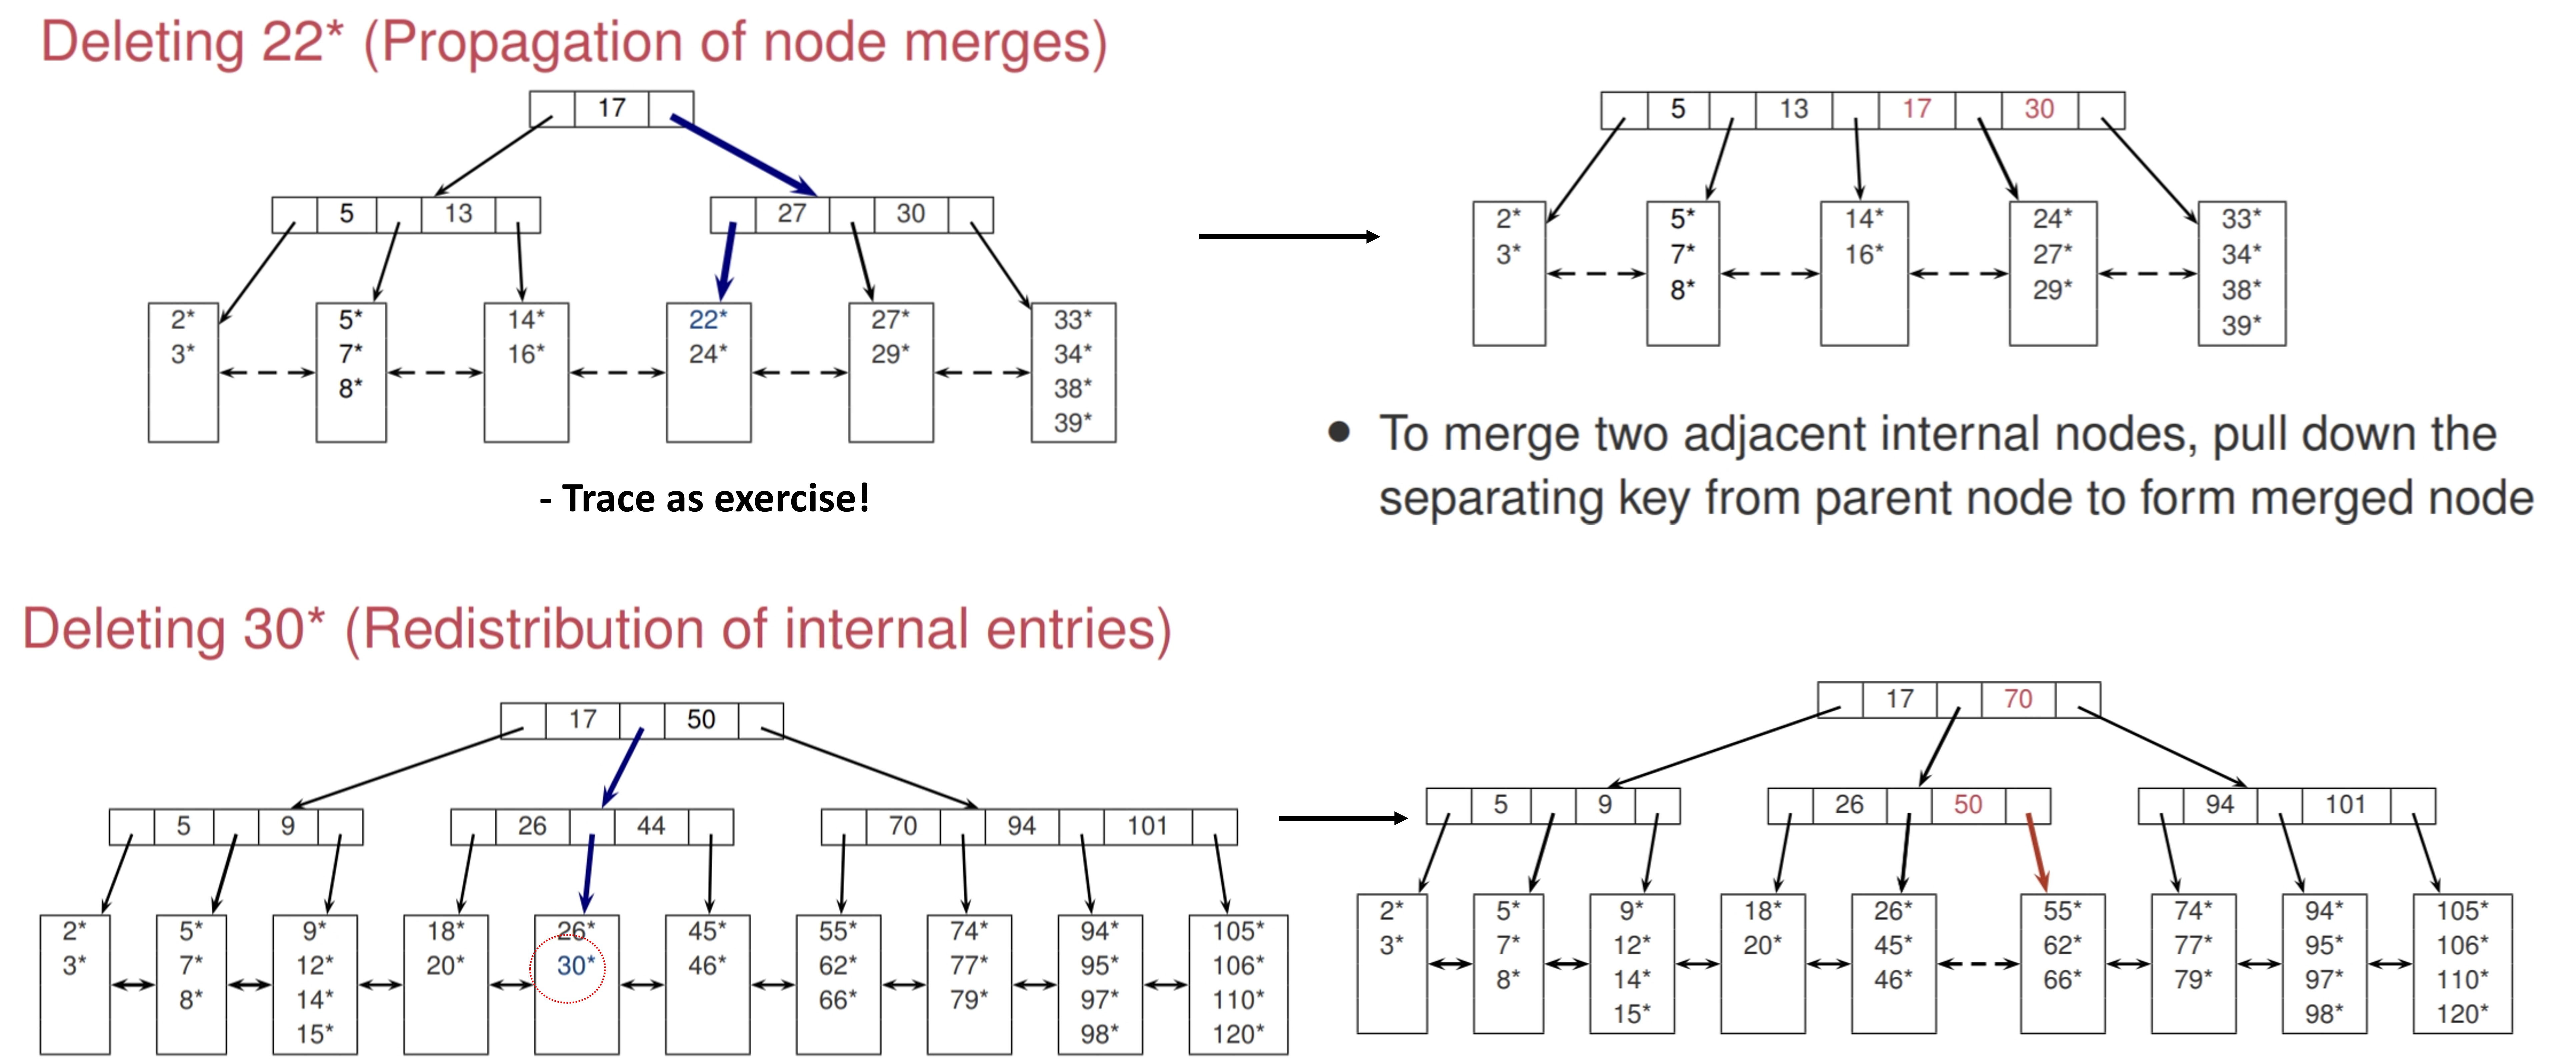
\includegraphics[width = 1\linewidth]{Bdeletion2}}
\begin{itemize}
\item Chances are high that redistribution is possible if node has two siblings, and unlike merging, redistribution is guaranteed to propage no further than parent node. Also, pages have more space, reducing likelihood of split on subsequent insertions.
\end{itemize}

\columnbreak

\subsection{$B^+$-Tree Bulk Loading}
\begin{itemize}
\item Entries added to a $B^+$ in two ways.
	\begin{enumerate}
	\item Have existing collection of data records with $B^+$ tree index on it. When record added to collection, corresponding entry added to $B^+$ tree. (Insert, Delete individually)
	\item Have collection of data records we want to create new $B^+$ tree index on some key field(s). Start with an empty tree. Inserting one by one expensive dur to overhead, systems provide \textbf{bulk loading} utility.
	\end{enumerate}
\item \textbf{Bulk Loading}: 
	\begin{enumerate}
	\item Sort data entries $k*$ to be inserted into $B^+$ tree according to search key $k$. (Here, $d$ = 1).
	\item Allocate empty page to serve as root. Insert a pointer to first page of (sorted entries into it).
	\centerline{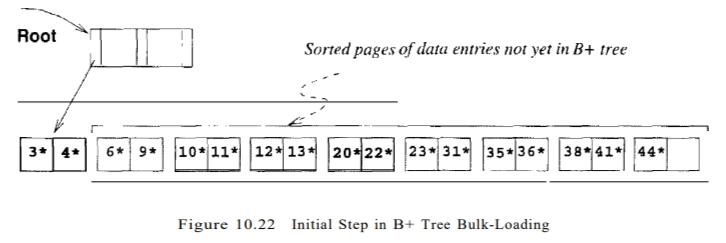
\includegraphics[width = 0.8\linewidth]{bulkloading1}}
	\item Add one entry to root page for each page of sorted data entries. Proceed until root page is full. Here, we must split root and create a new root page.
	\centerline{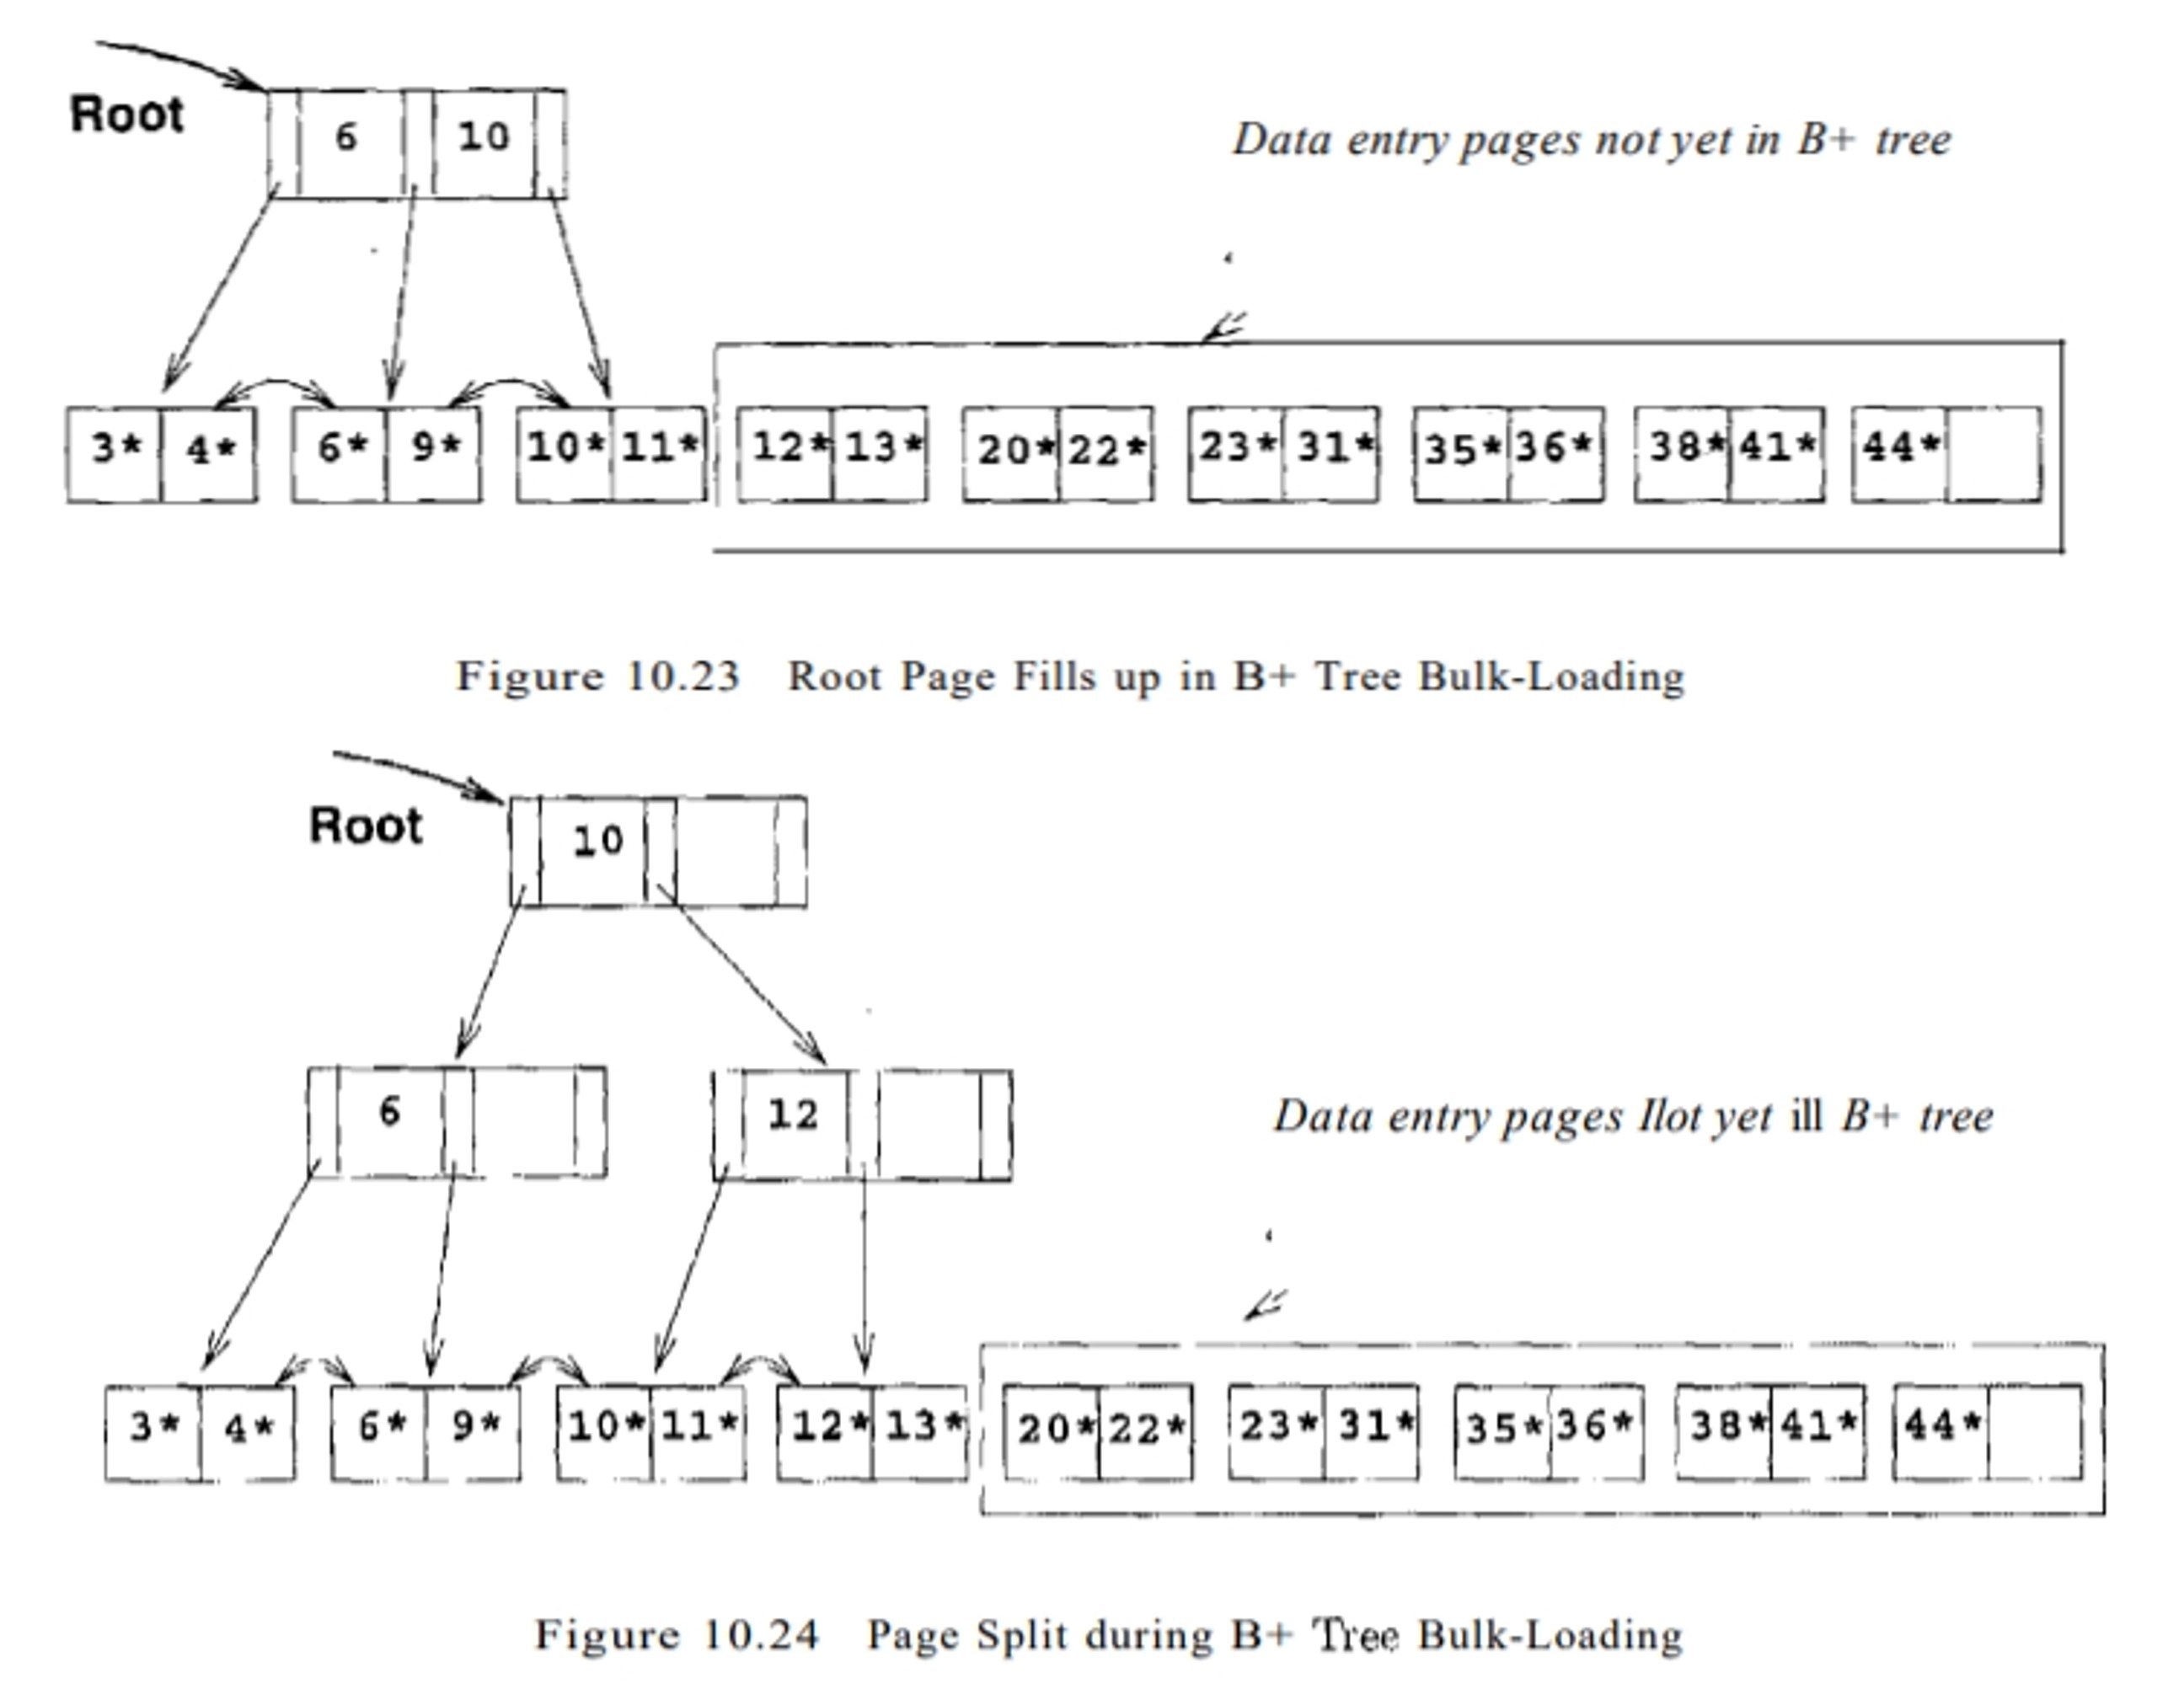
\includegraphics[width = 0.8\linewidth]{bulkloading2}}
	\item To continue, entries for leaf pages \textbf{always inserted into right-most index page just above the leaf level}. When right-most page above leaf level fills up, it is split.
	\centerline{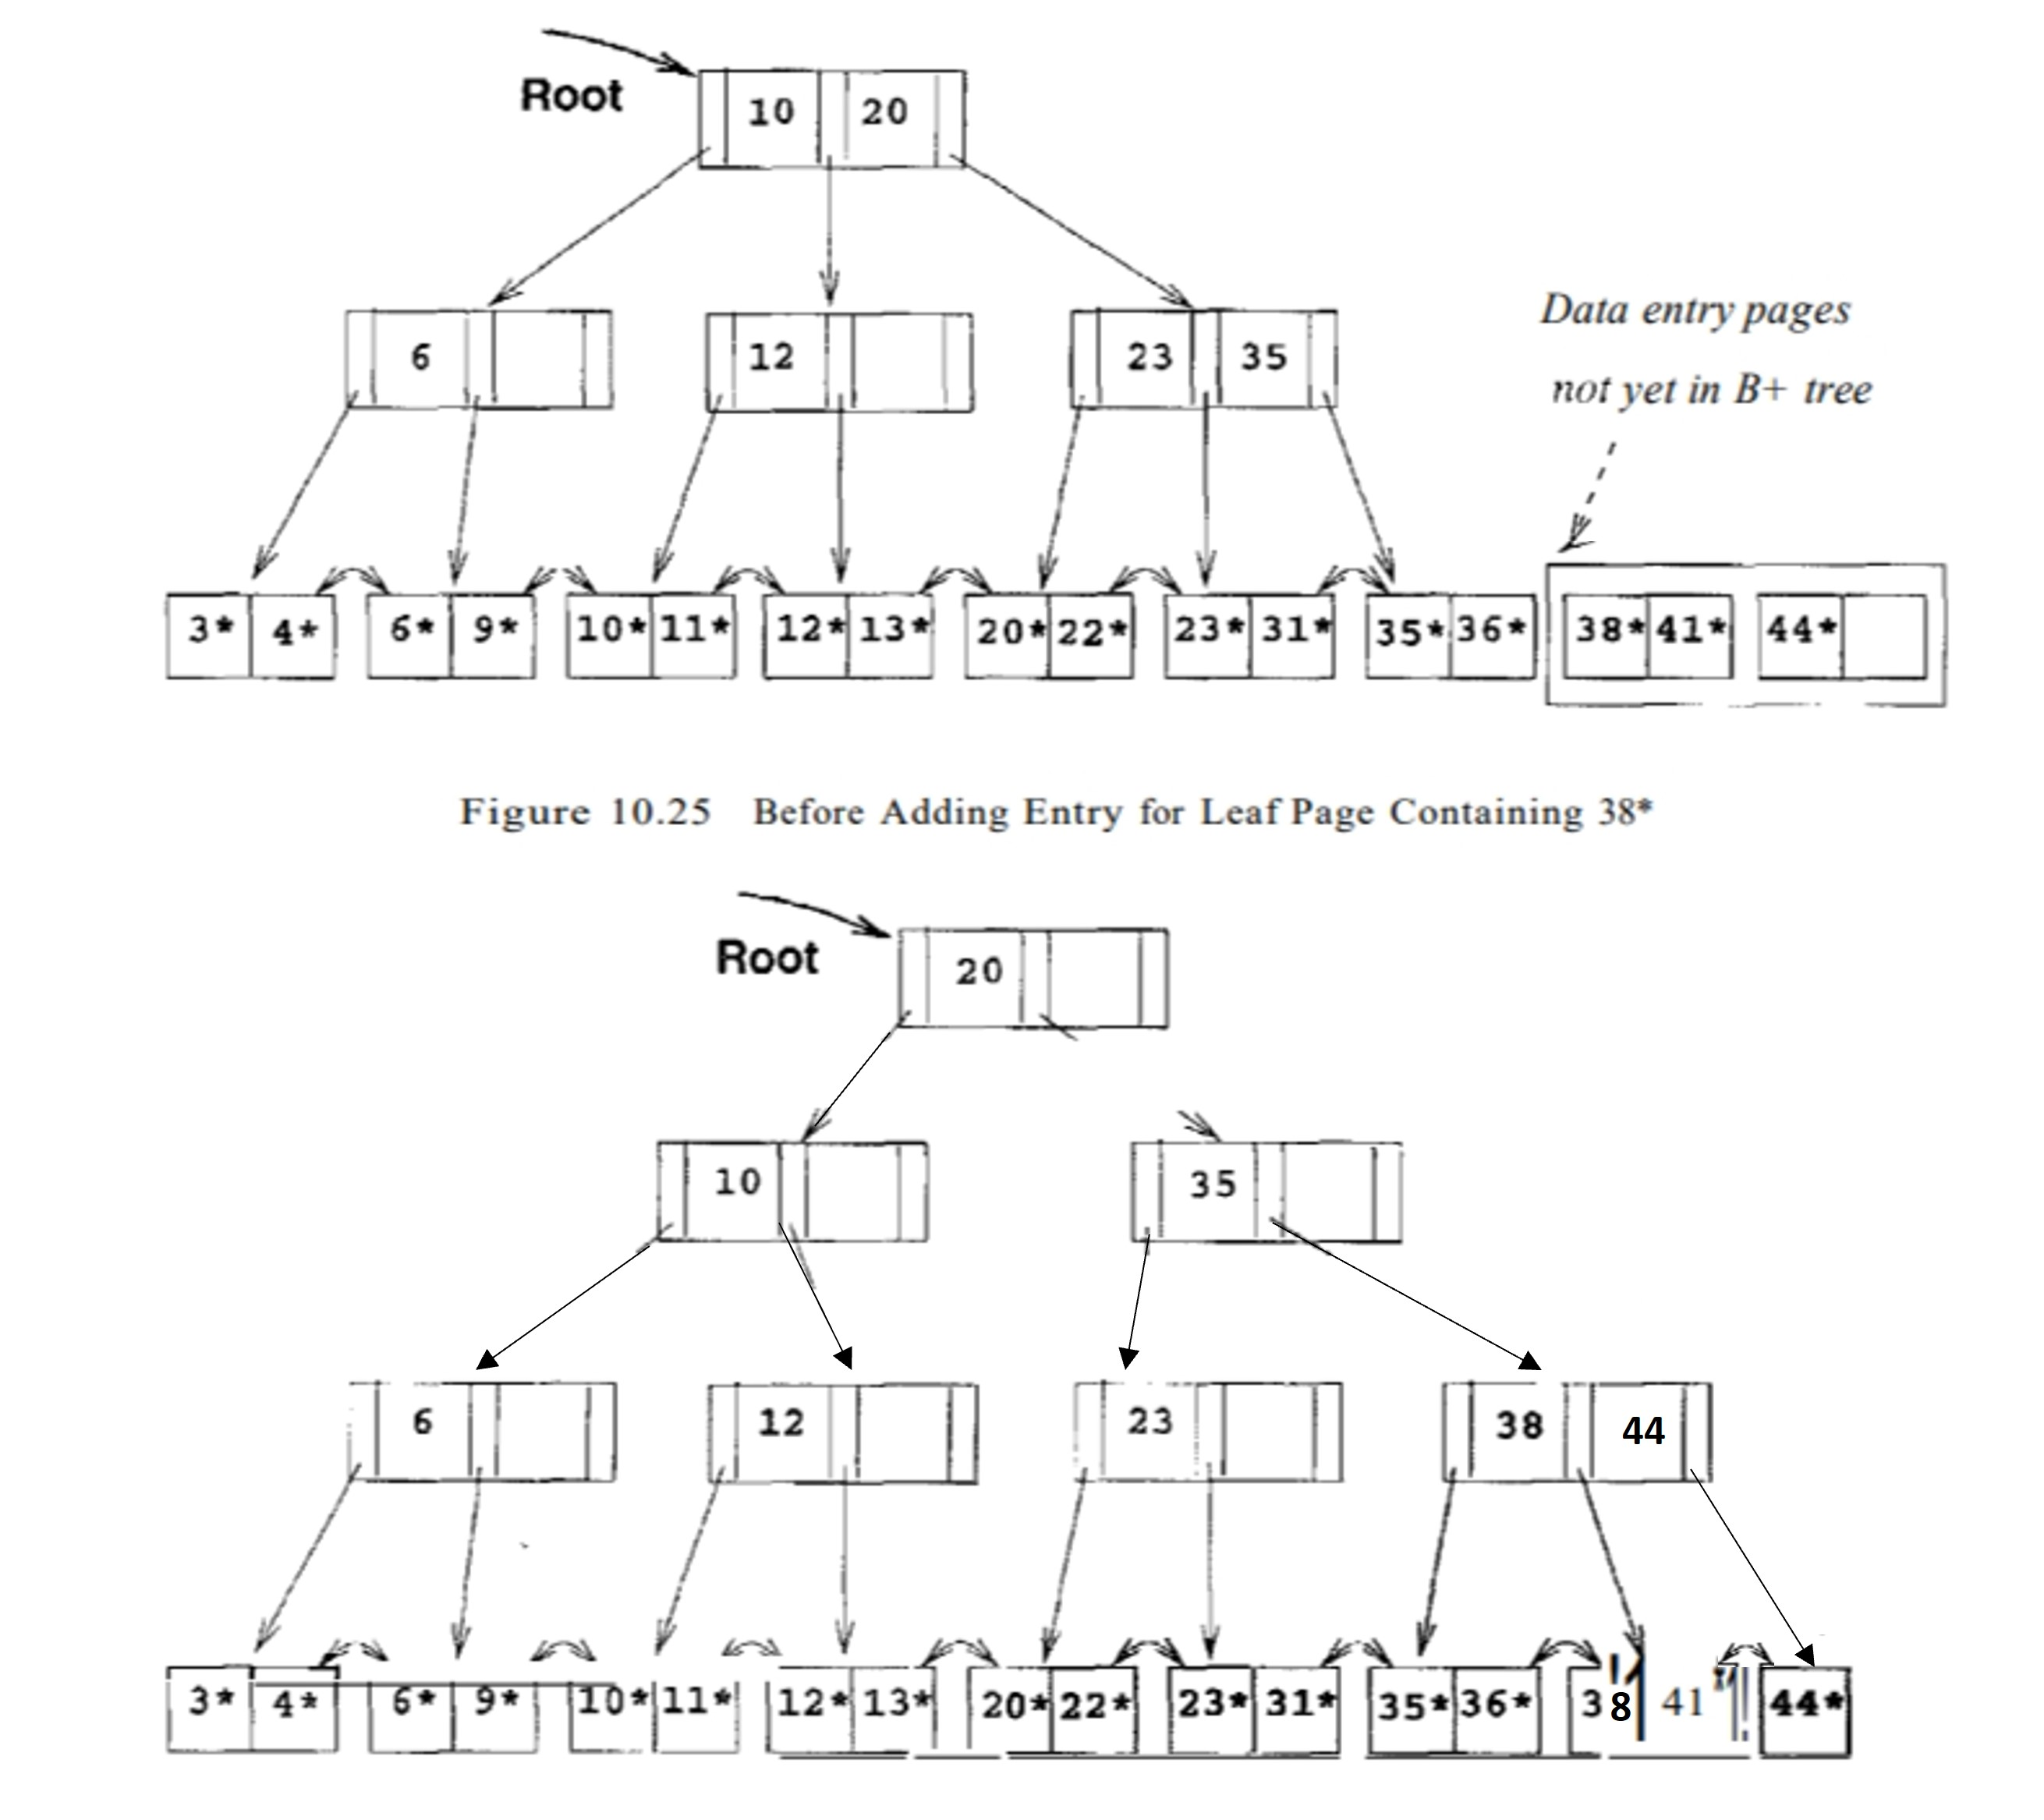
\includegraphics[width = 0.7\linewidth]{bulkloading3}}
	\end{enumerate}
\end{itemize}

\section{3. Hash-based Indexing}
\begin{itemize}
\item Used for \textbf{equality queries}, not for range queries.
\item \textbf{Hashing techniques}: \textbf{Static hashing, dynamic hashing} (linear hashing, extendible hashing, etc).
\end{itemize}

\subsection{Static Hashing}
\begin{itemize}
\item \textbf{Data stored in $N$ buckets}, fixed at creation time. Bucket consists of \textbf{one primary data page \& chain} of zero or more overflow data pages.
\item $v$* represents data entry $e$ with h(e.key) = $v$, not search entry with RID. 
\item \textbf{Problem with static hashing}: As data grows, longer overflow chain, efficiency drops. Need to periodically rehash and increase no. of buckets.
\end{itemize}
\centerline{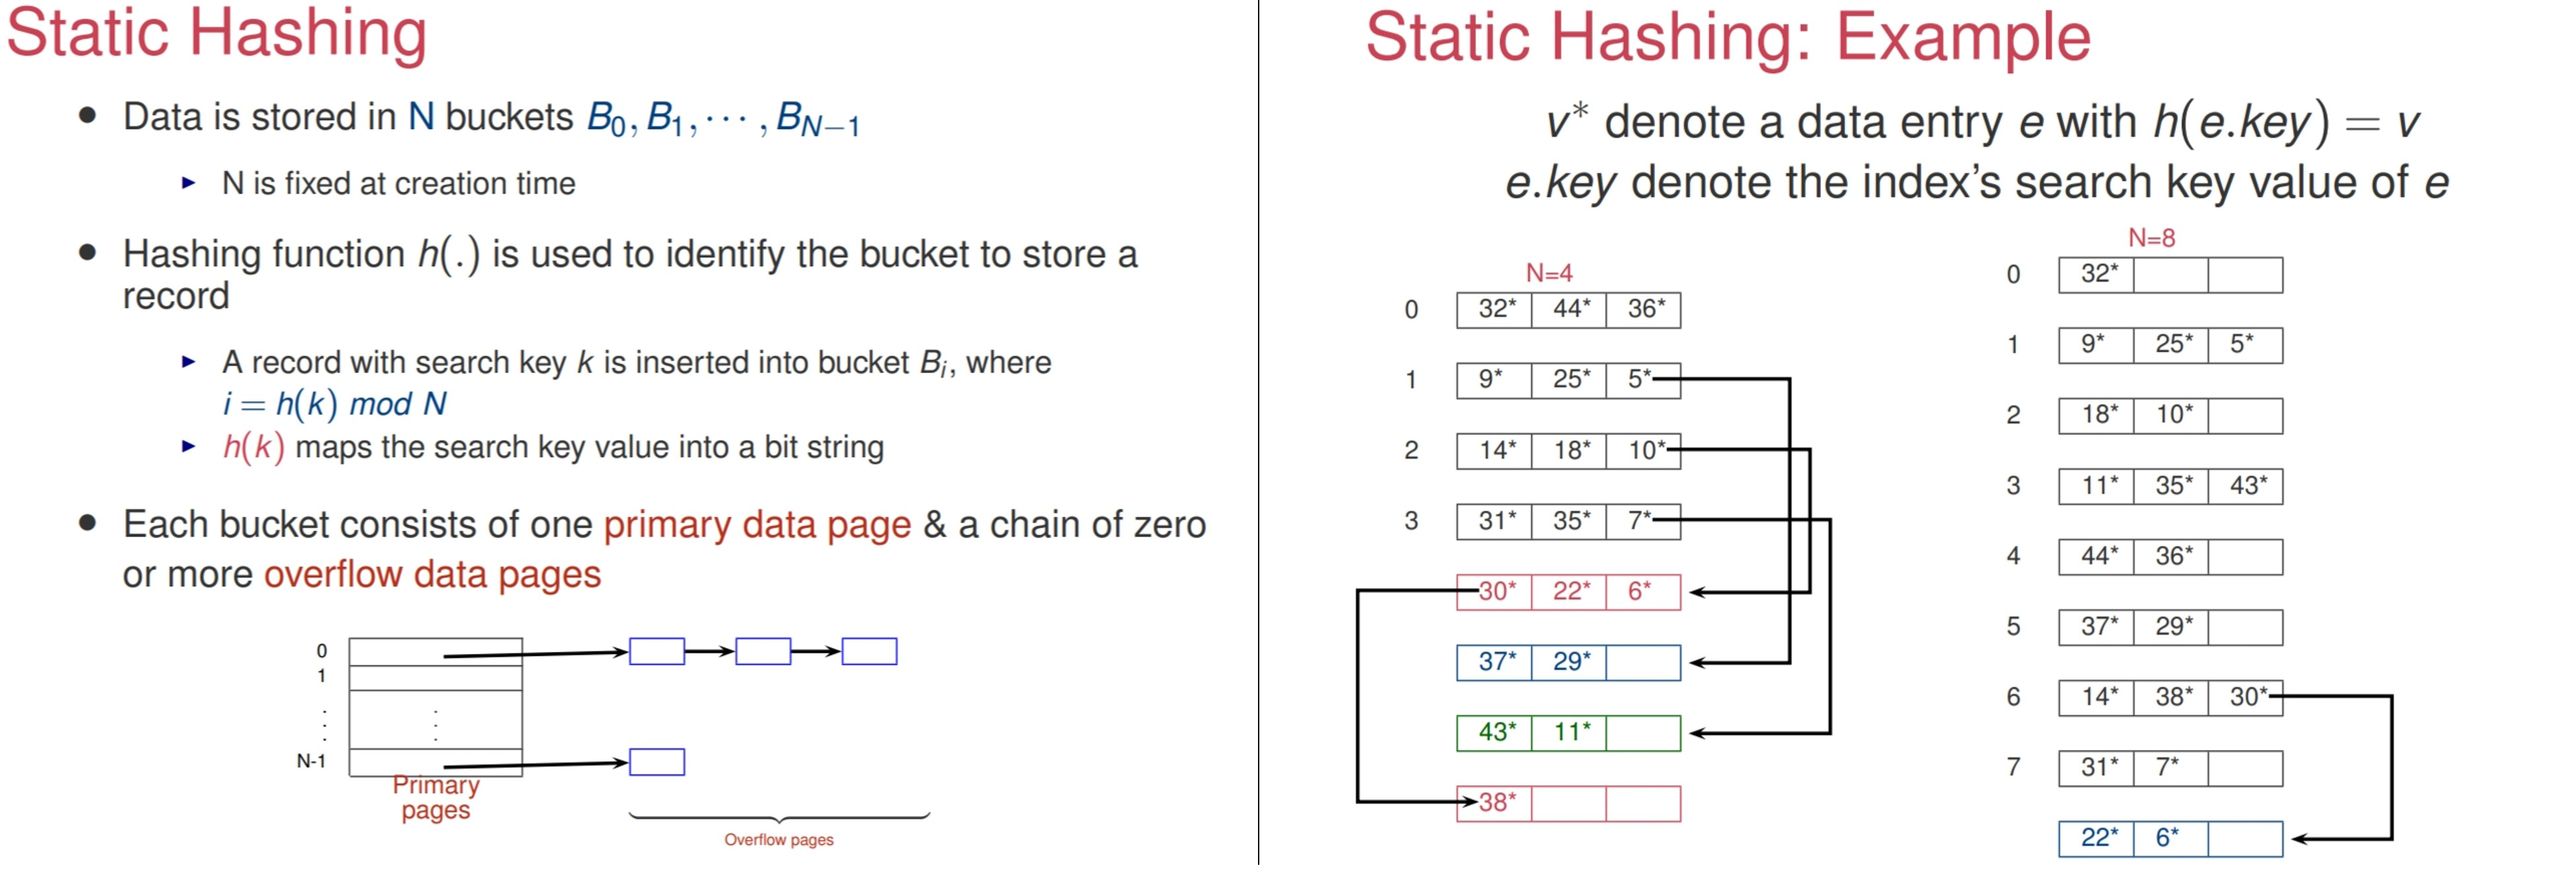
\includegraphics[width = 0.95\linewidth]{staticHashing}}


\subsection{Dynamic Hashing: Linear Hashing}
\begin{itemize}
\item Hash file grows / shrinks linearly, systematic \textbf{splitting of buckets}.
\item Overflow pages needed as overflowed bucket may not be split immediately. 
\item Hashing function changes dynamically and at given instant, \textbf{at most two (successive) hashing functions} used by the scheme during search.
\item Each bucket has primary data page \& chain of zero+ overflow pages.
\item Insert in bucket $B_i$ overflows if all pages in $B_i$ (primary + overflow) full.
\end{itemize}
\centerline{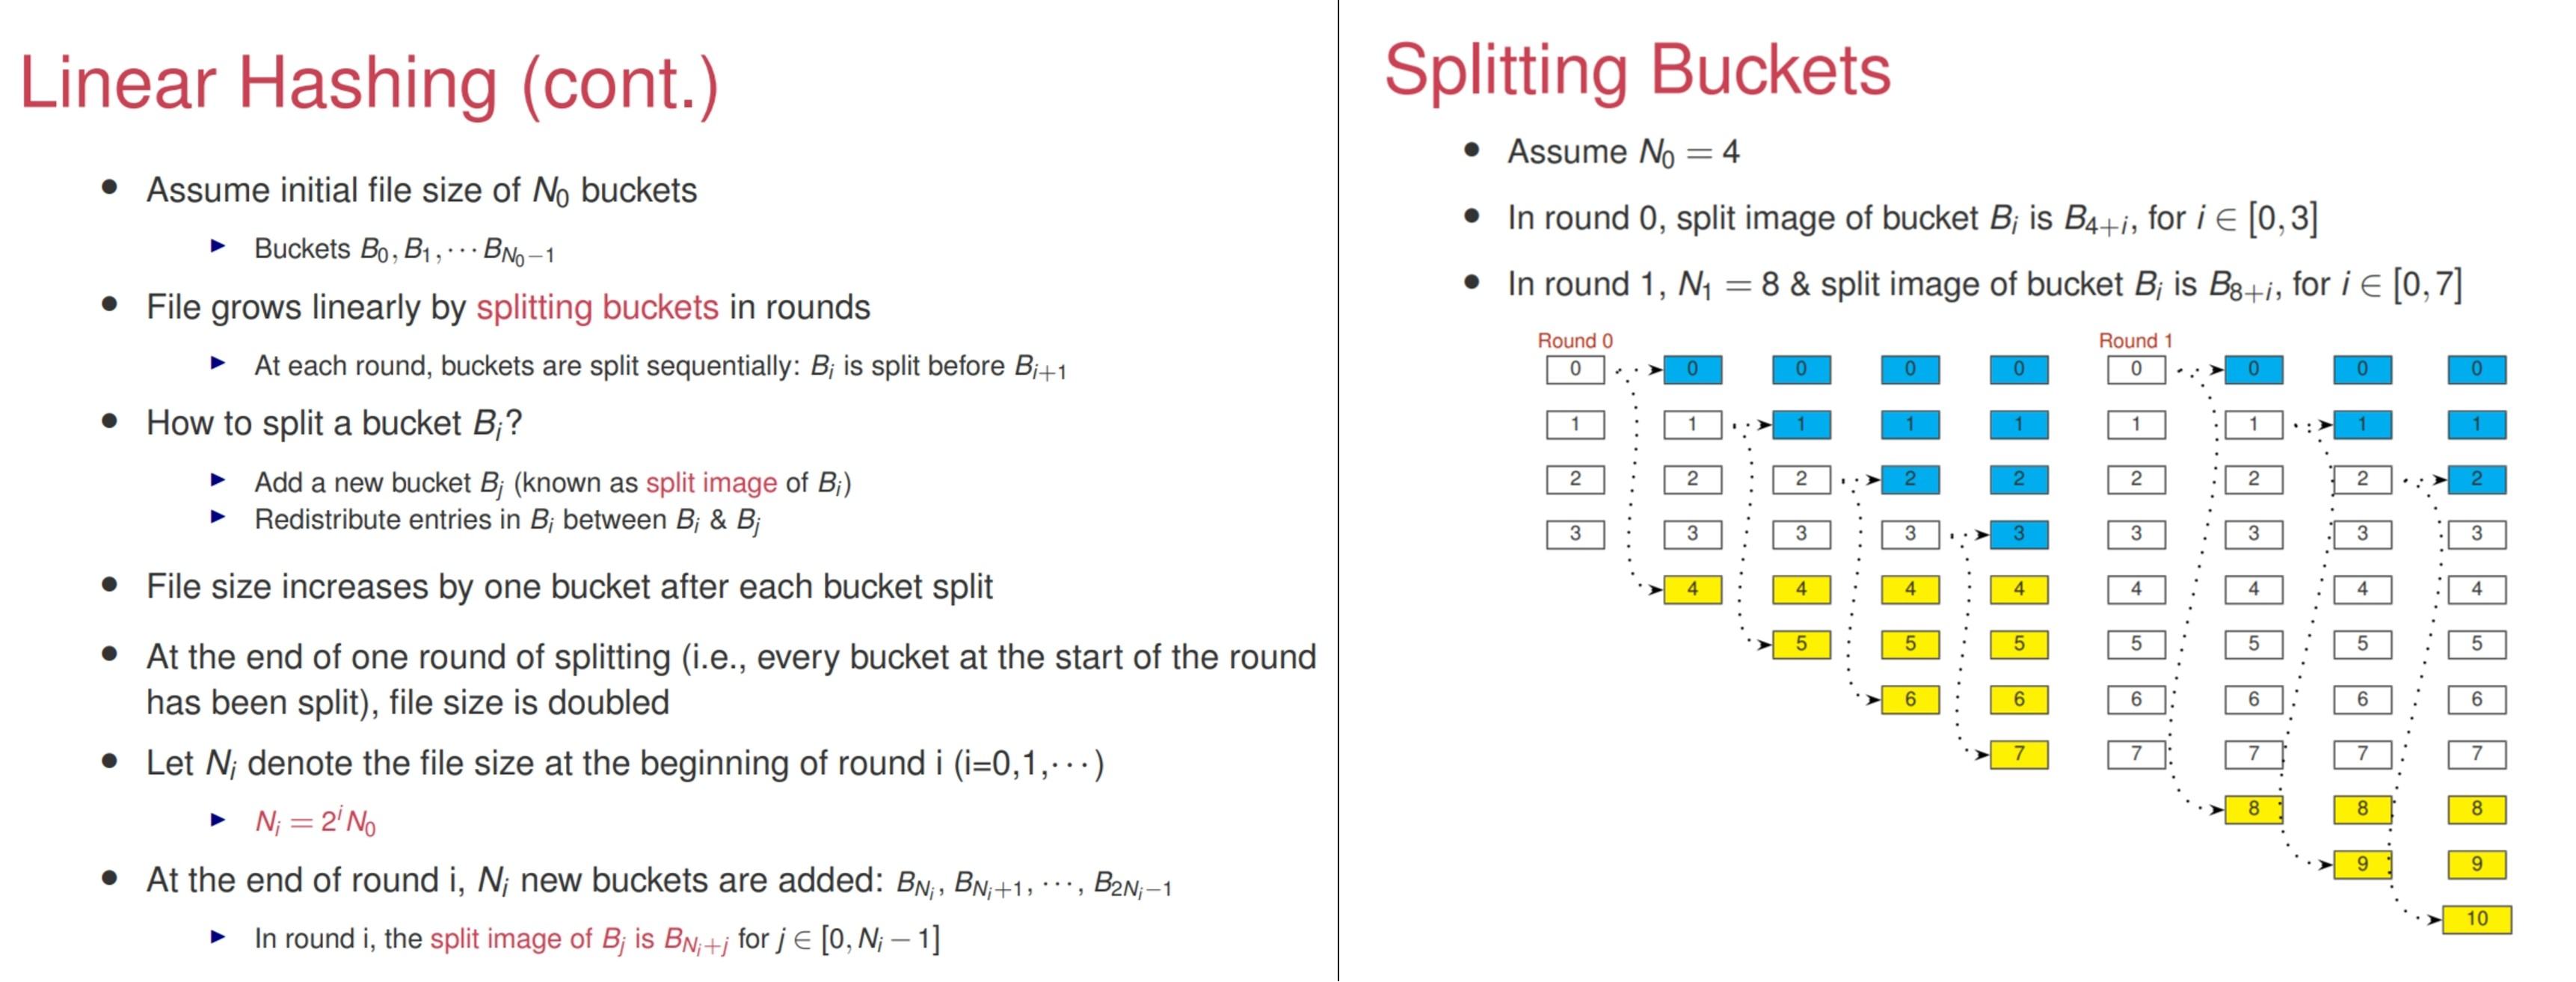
\includegraphics[width = 1\linewidth]{linearHashing}}

\subsubsection{Dynamicity of Linear Hashing}
\centerline{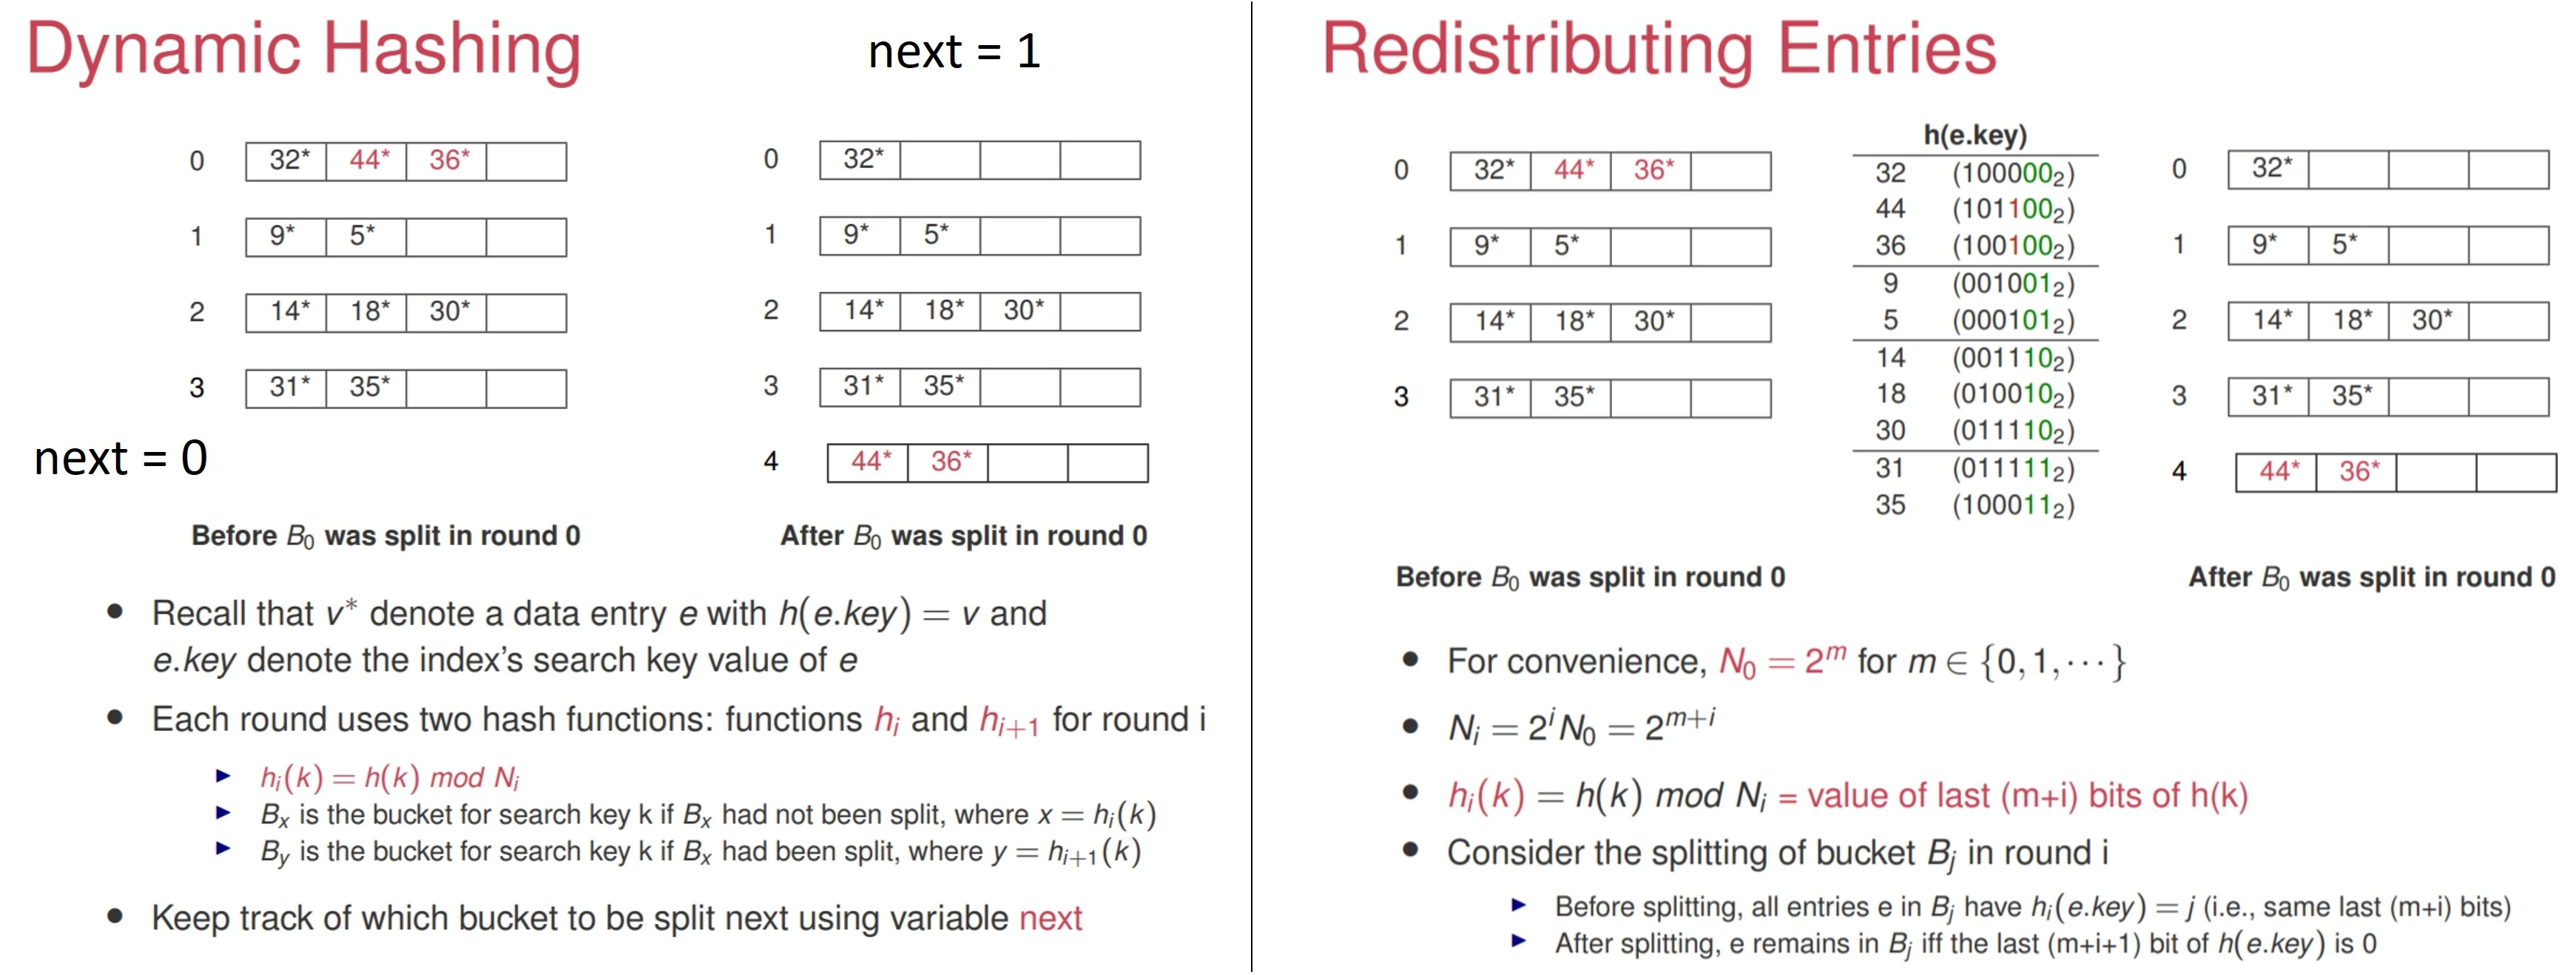
\includegraphics[width = 1\linewidth]{dynamicHashing}}

\subsubsection{Linear (Hashing) Splitting of Buckets (Insertion)}
\begin{itemize}
\item Number in buckets represent the rightmost bit values.
\item \textbf{Split Criteria}: variable, could be when some bucket overflow, space utilization of file above some threshold etc.
\item \textbf{Level}: We use level to denote splitting round number (use with \textbf{next}).
\end{itemize}
\centerline{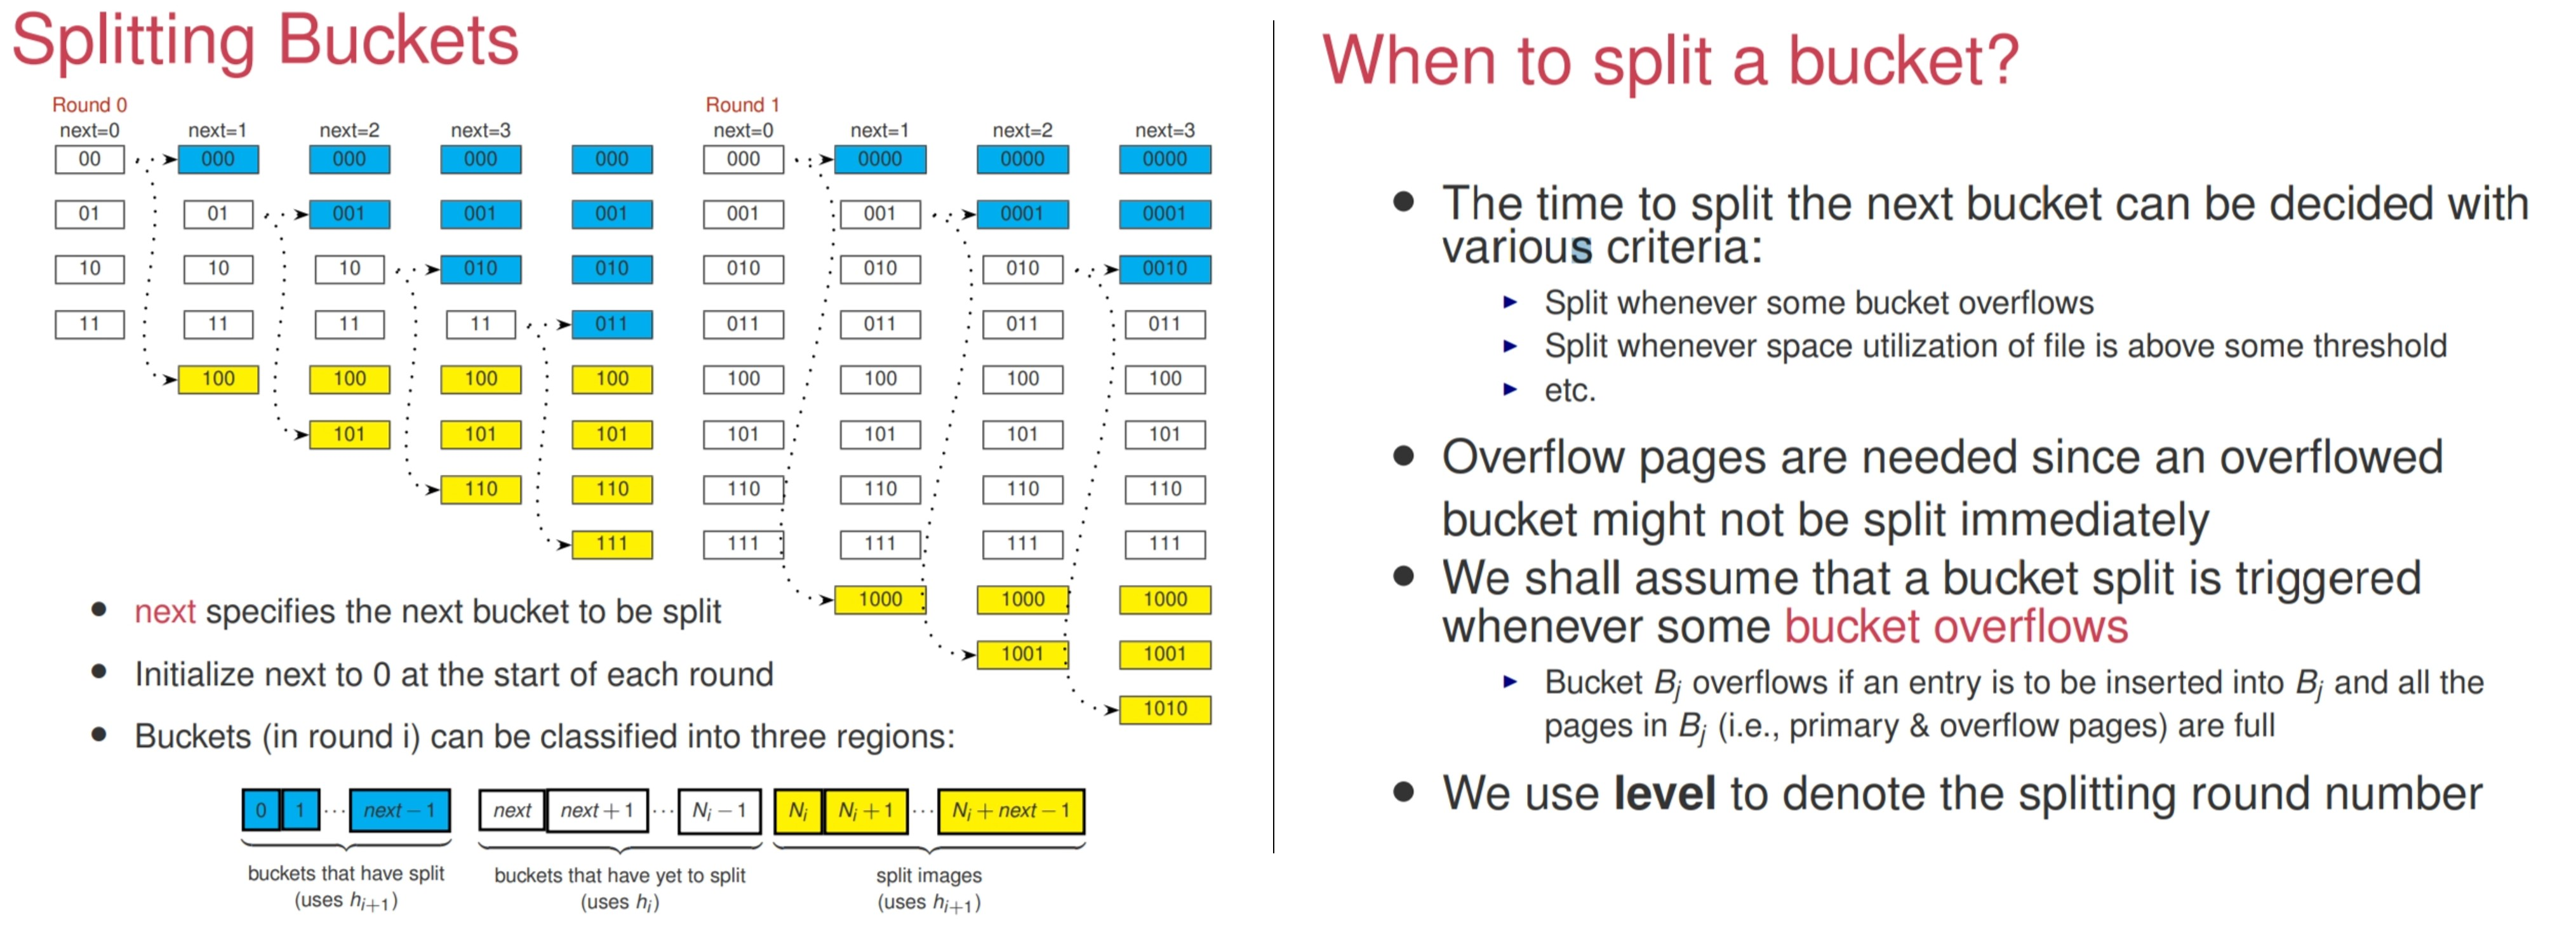
\includegraphics[width = 1\linewidth]{splitBucket}}

\subsubsection{Examples: Linear Hashing Search \& Insert}
\begin{itemize}
\item Even though overflowed bucket split, not neccessary mean enough space if bit value not right. Still require overflow page.
\item Using \textbf{level and next}, we determine how many additional bits to consider in \textbf{second hashing function}.
\item \textbf{Second hashing function}: Is simply looking at the m rightmost bits of the hash.
\end{itemize}
\centerline{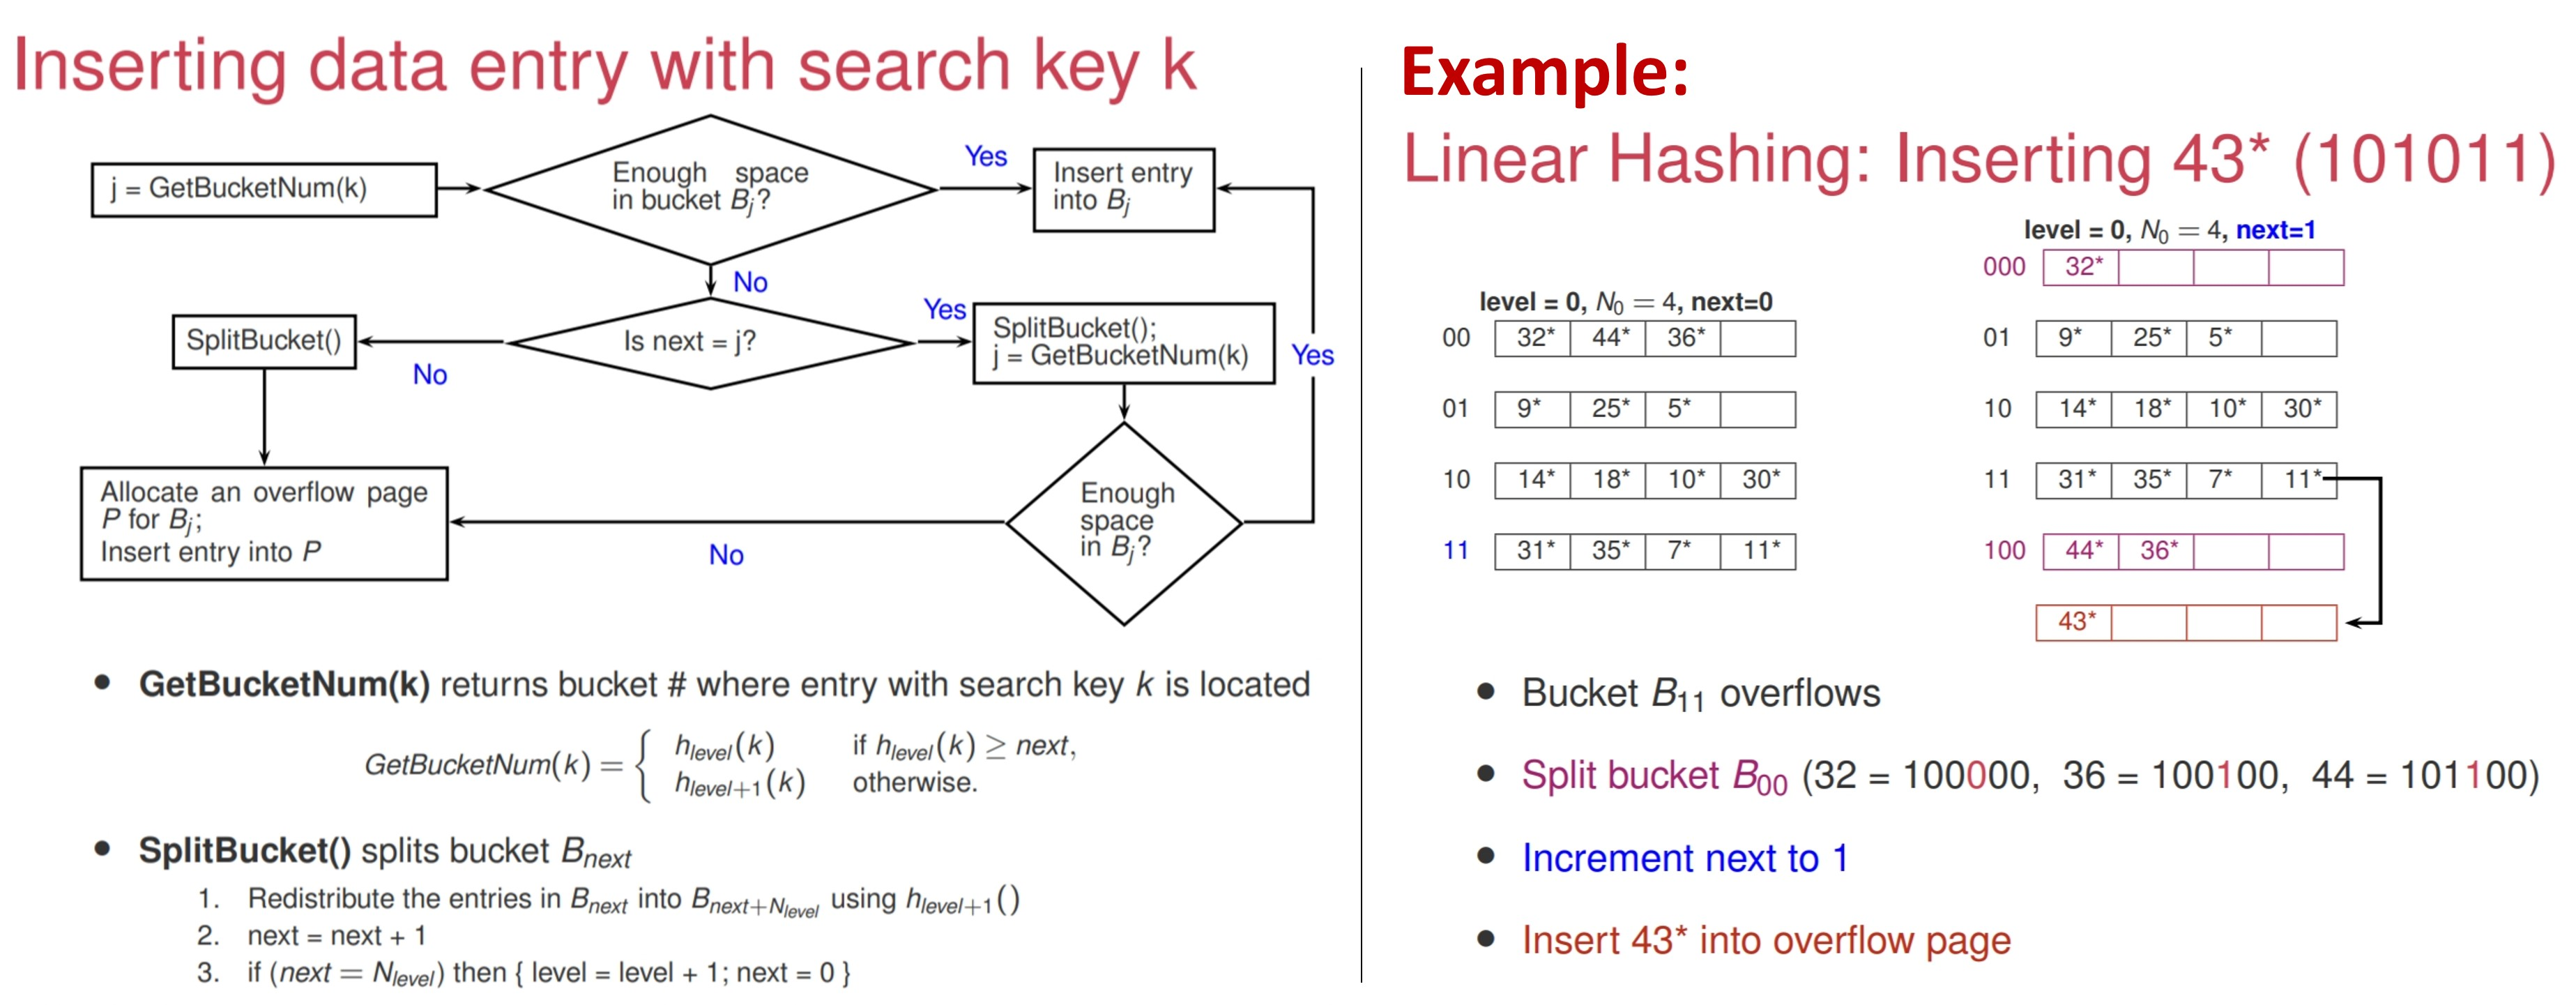
\includegraphics[width = 0.9\linewidth]{splitBucket1}}
\centerline{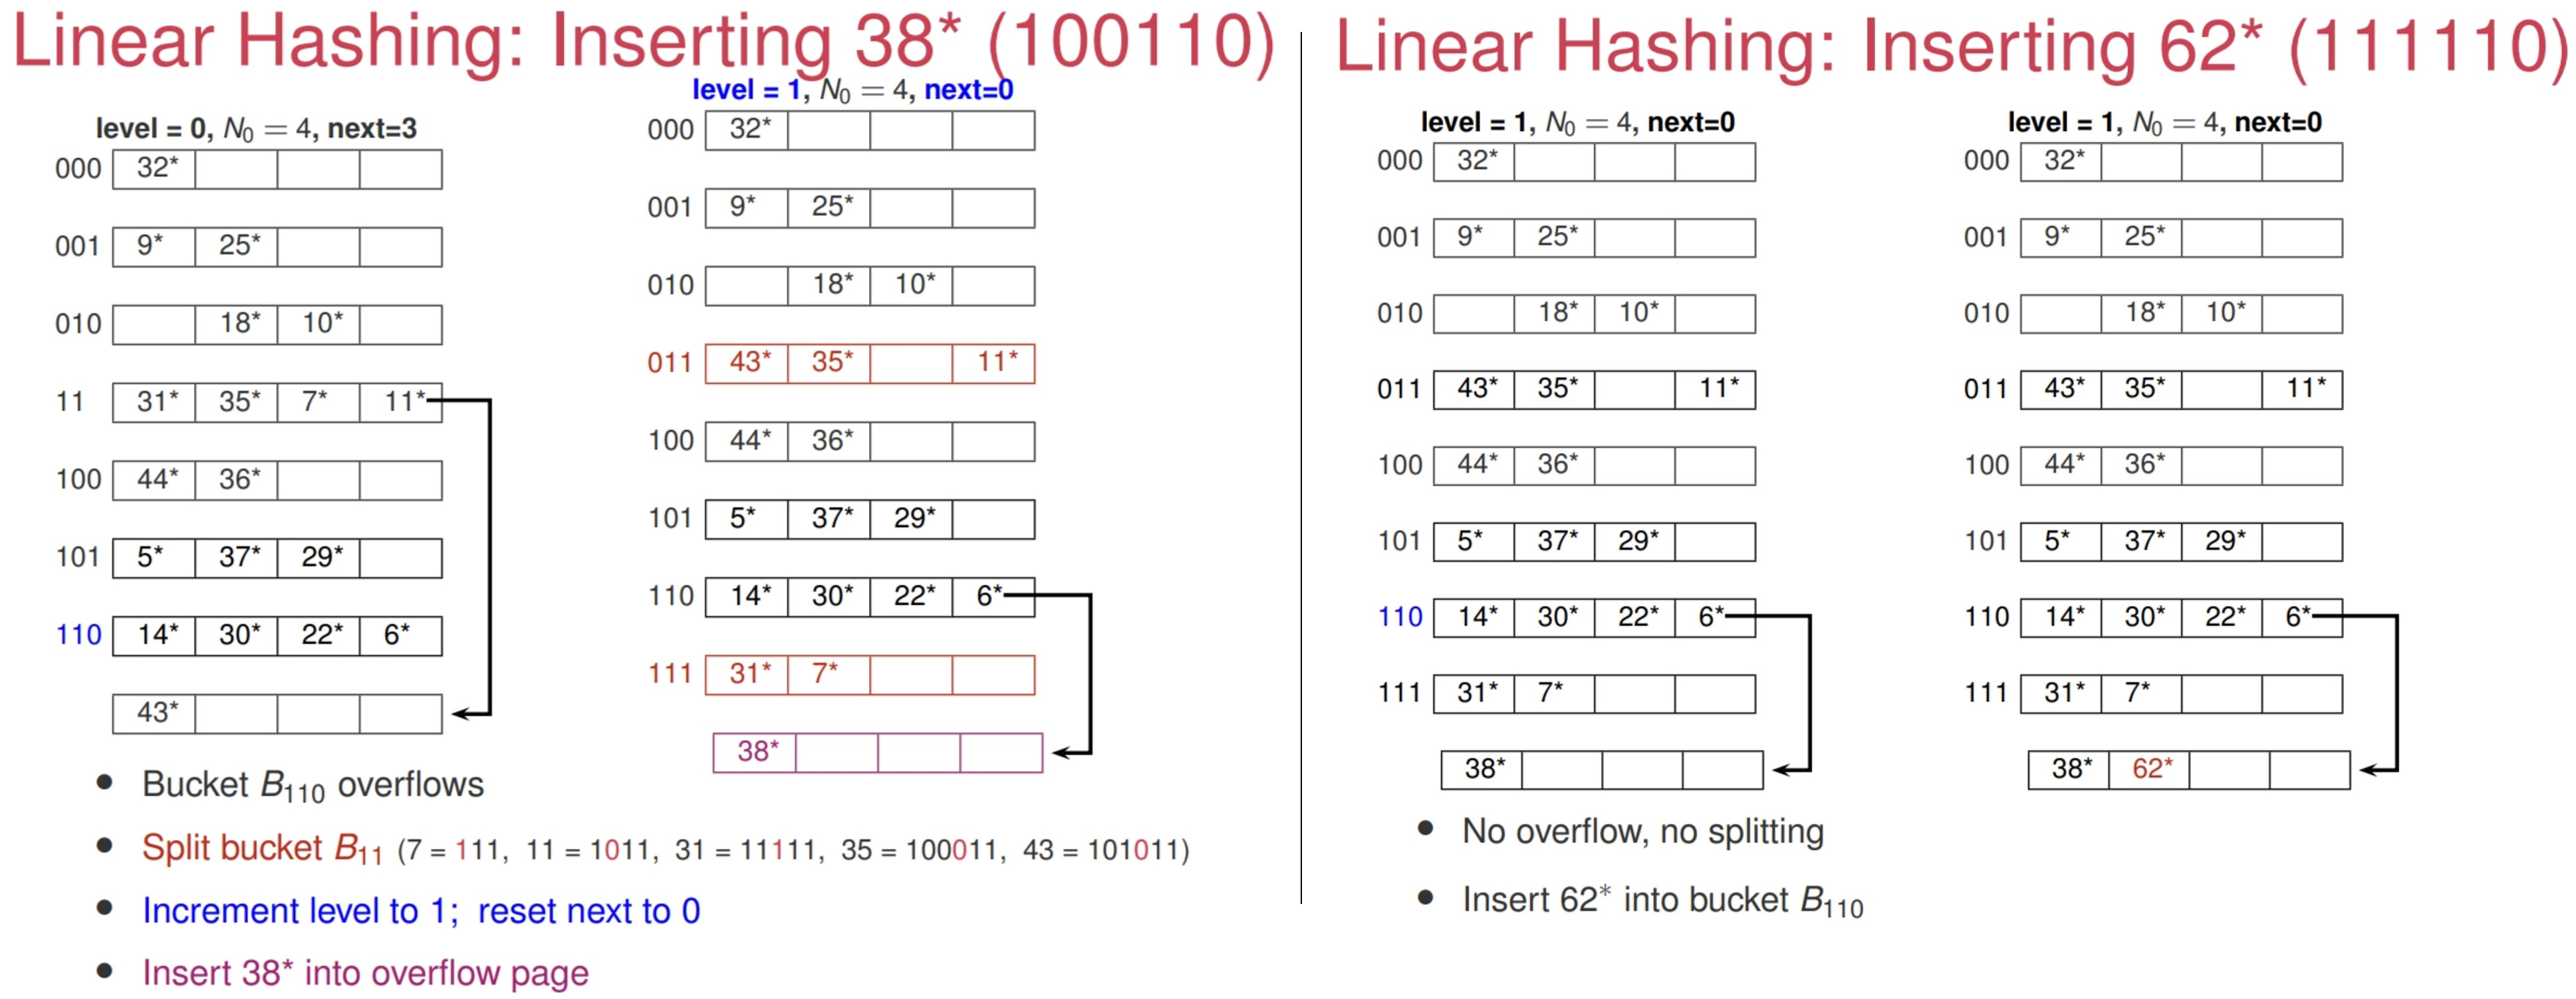
\includegraphics[width = 0.85\linewidth]{splitBucket2}}

\subsubsection{Linear Hashing Deletion}
\begin{itemize}
\item Opposite of insertion.
\item \textbf{Two cases}: 1. (Next > 0), 2. (Next = 0, and level $>$ 0.)
\end{itemize}
\centerline{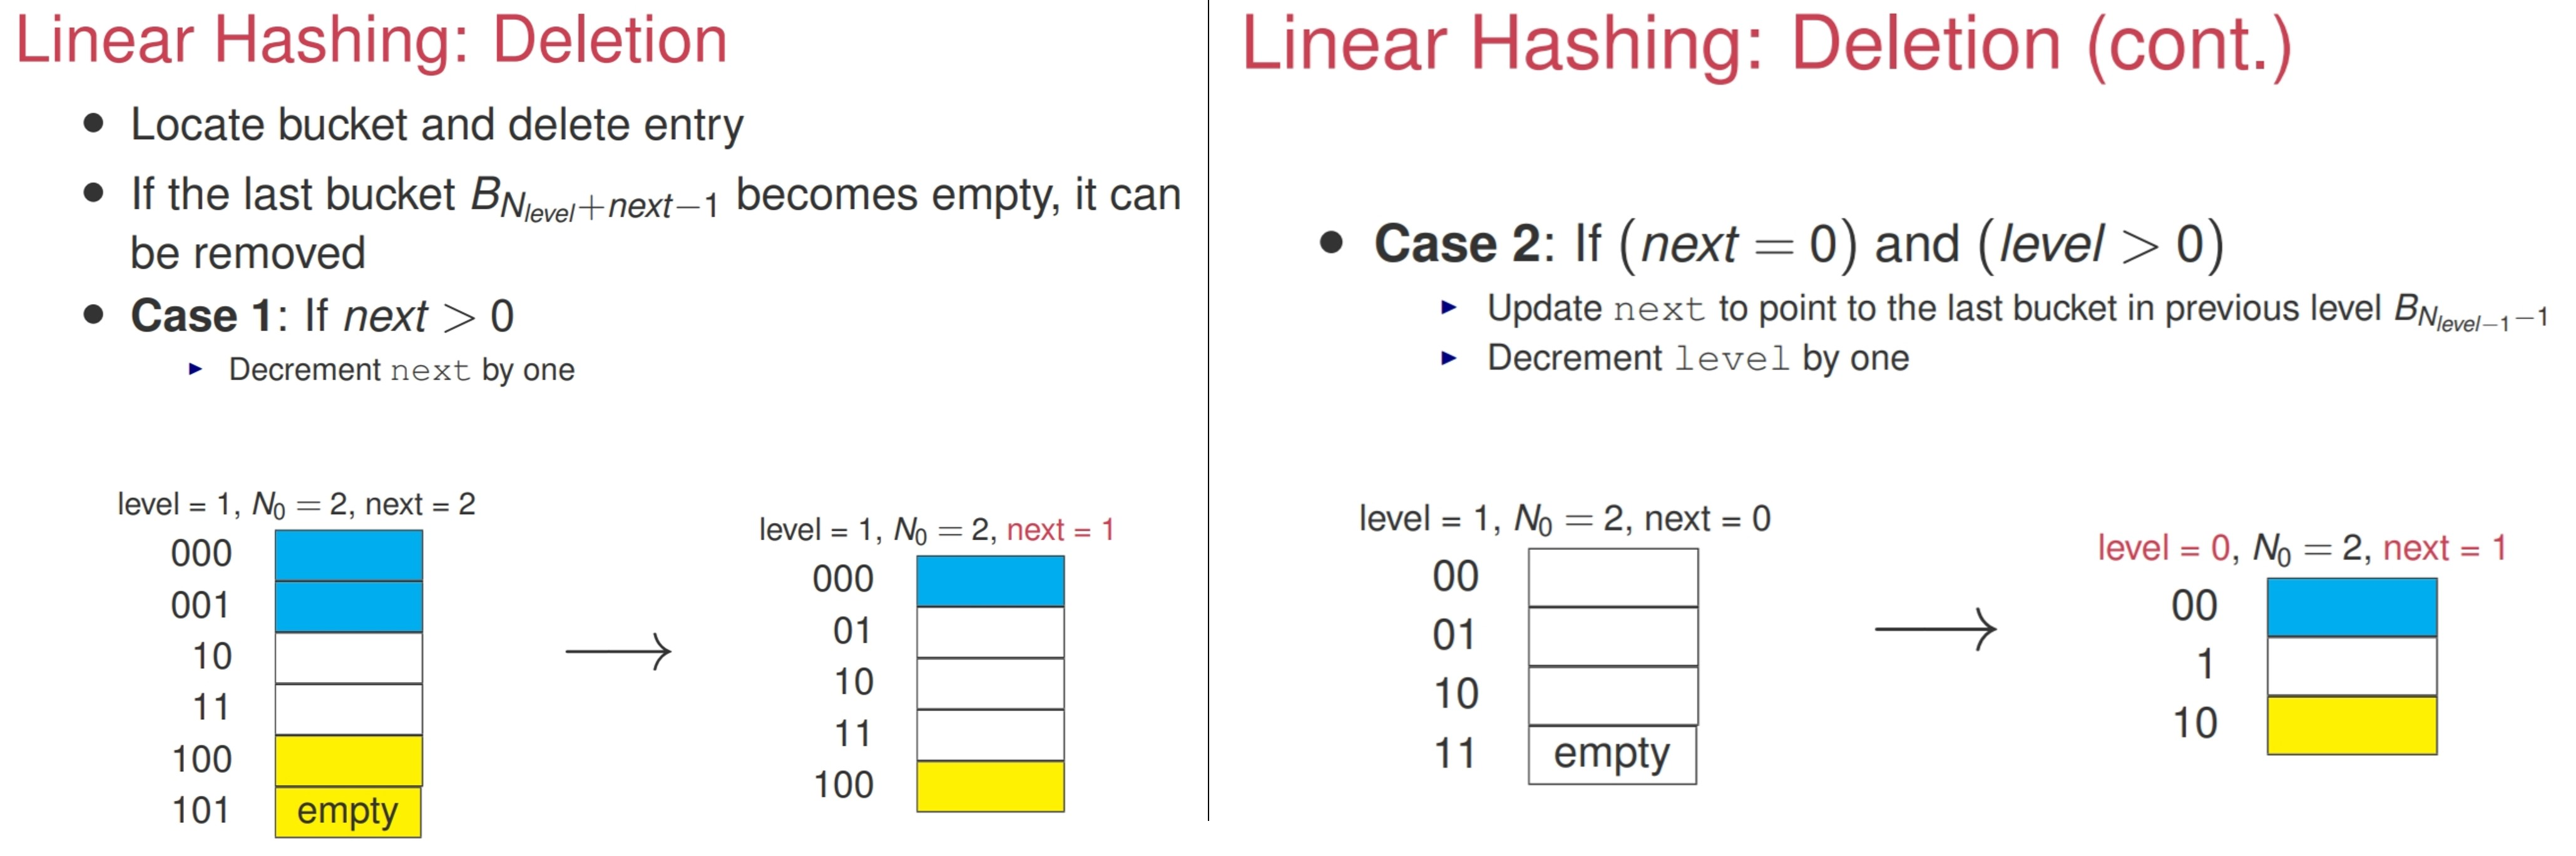
\includegraphics[width = 1\linewidth]{deletionBucket}}

\subsubsection{Linear Hashing Performance, Summary}
\centerline{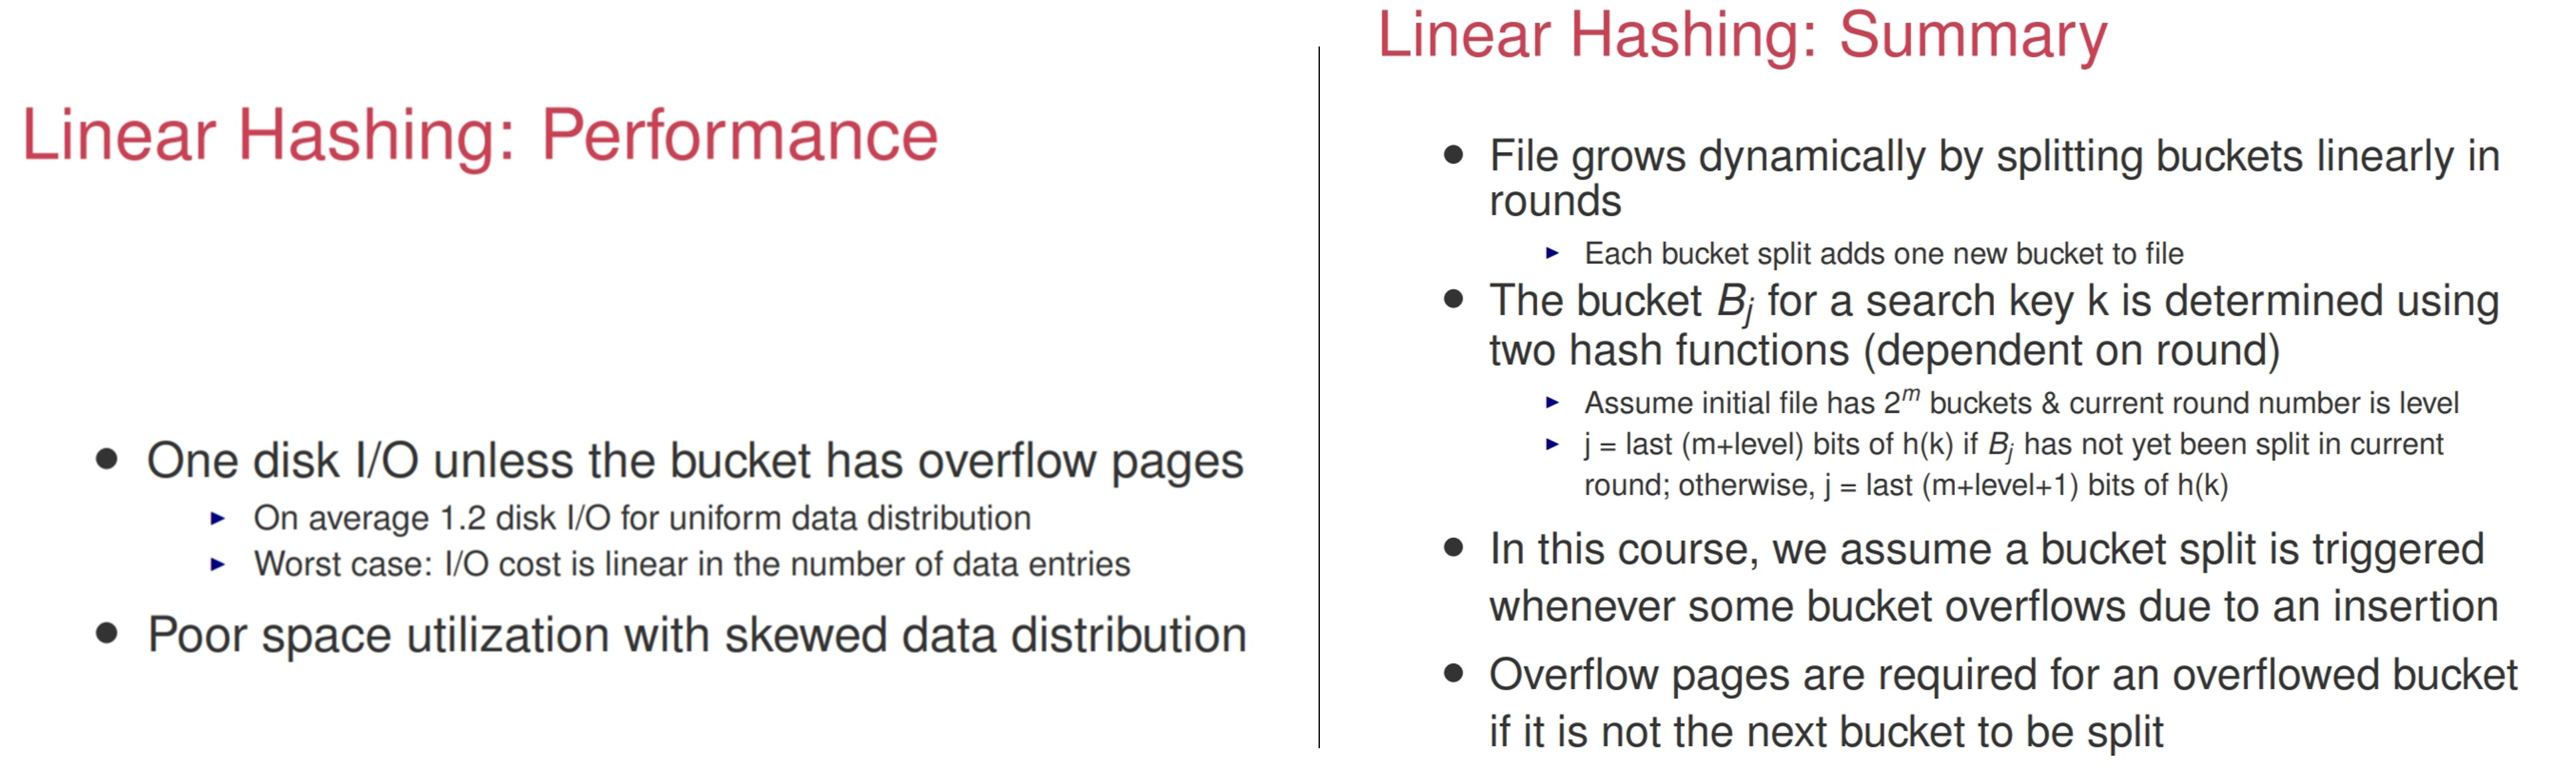
\includegraphics[width = 1\linewidth]{linearHashingSummary}}

\columnbreak

\subsection{Dynamic Hashing: Extendible Hashing}
\begin{itemize}
\item \textbf{Similar to Linear Hashing}: we want \textbf{bucket number to grow dynamically}, and use some \textbf{number of least significant bits} of h(k) to determine bucket address for search key $k$.
\item \textbf{Difference}: Add new bucket (as split image) when existing bucket overflows, No overflow pages (except when number of collisions exceed page capacity, two page entries collide if they have same h(.) hash value).
\end{itemize}

\subsection{Extendible Hashing}
\begin{itemize}
\item \textbf{Extendible hashing}: dynamically updateable disk-based index structure, implements hashing scheme utilizing a \textbf{directory of pointers to buckets}. 
\item Overflows handled by doubling the directory which logically doubles the number of buckets. \textbf{Physically, only the overflown bucket is split}.
\end{itemize}
\centerline{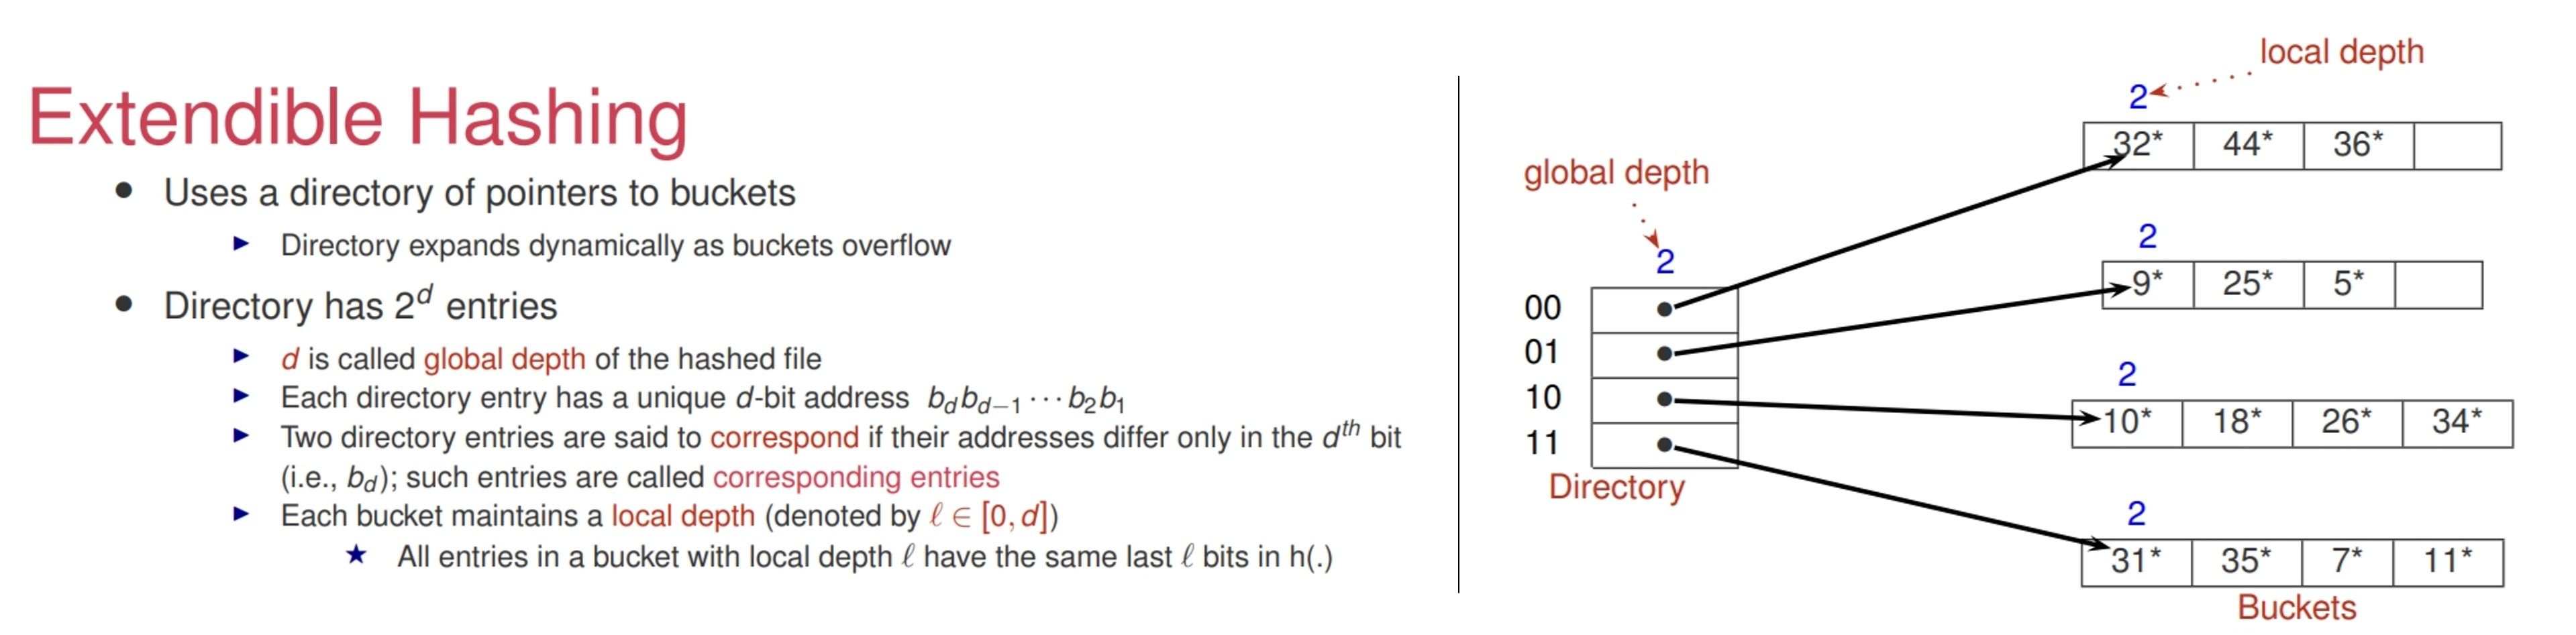
\includegraphics[width = 1\linewidth]{extendibleHashing}}

\subsubsection{Extendible Hashing Performance}
\begin{itemize}
\item \textbf{Performance}: At most 2 disk I/O for equality selection, at most 1 I/O if directory fits in main memory.
\item \textbf{Handling collision}: Two data entries \textbf{collide} if same hashed value, overflow pages need when number of collisions exceed page capacity.
\item Compared with B+-tree index exact match queries (log number of I/Os), E. Hashing better expected query cost O(1) I/O. 
\end{itemize}

\subsubsection{Extendible Hashing: Handling Bucket Overflow}
\begin{itemize}
\item Main idea: Determine if there is empty directory entry to point to new bucket. \textbf{2 Cases}: decision to split, or use empty directory entry.
\end{itemize}

\subsubsection{Case 1: Split bucket local depth = global depth}
\centerline{\includegraphics[width = 1\linewidth]{extendibleHashing1}}

\subsubsection{Case 2: Split bucket local depth $<$ global depth.}
\centerline{\includegraphics[width = 1\linewidth]{extendibleHashing2}}

\columnbreak

\subsubsection{Extendible Hashing Deletion}
\begin{itemize}
\item To delete entry, simply locate Bucket and delete. 
\item \textbf{Merging}: Mergable if entries can fit within a bucket, and same local depth, $j$ differs on in $l^{th}$ bit.
\end{itemize}
\centerline{\includegraphics[width = 1\linewidth]{extendibleHashing3}}

\section{4. Query Evaluation: Sorting \& Selection}
DBMS describes data it manages using tables, indexes (metadata), which is stored in special tables (system catalogs). This data used to find best way to evaluate a query.
\centerline{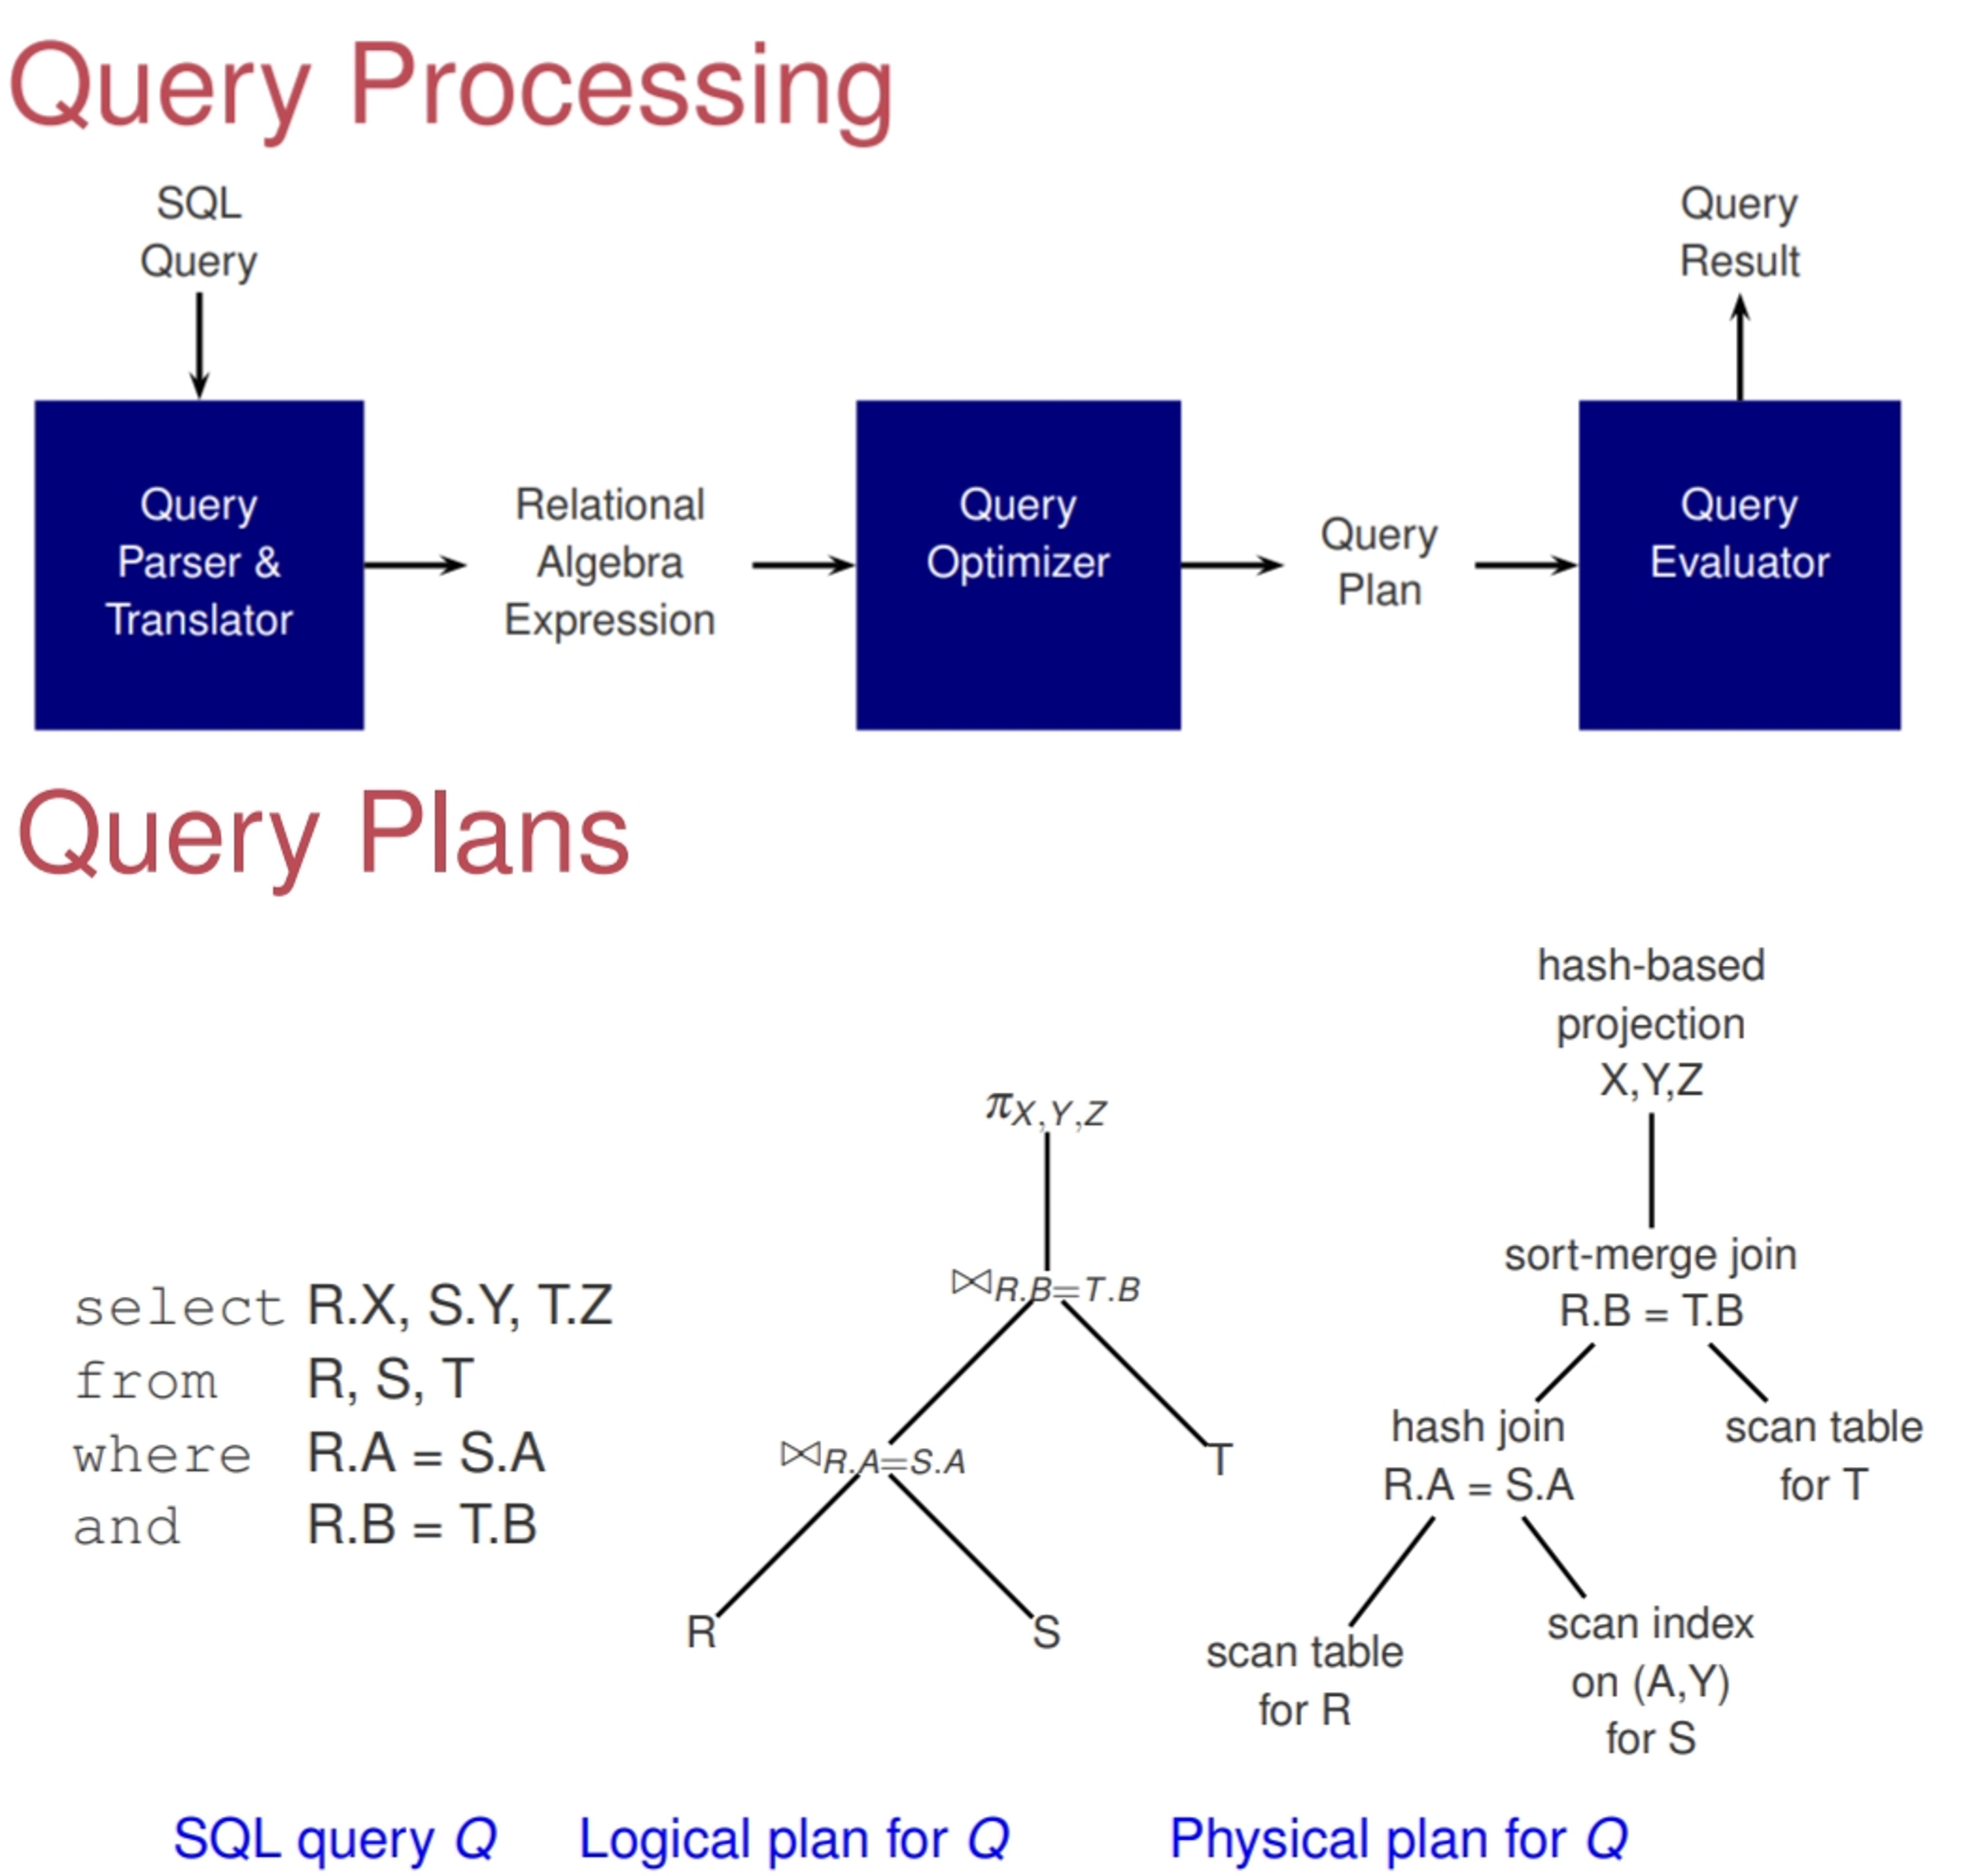
\includegraphics[width = 0.8\linewidth]{queryProcessing}}
\begin{itemize}
\item SQL queries translate into extended form of relational algebra
\item Query evaluation plans represented as tree of relational operators, with labels identifying algorithm to use at each node.
\item R. operators building blocks for evaluating queries, implementation of operators optimized for good perf.
\end{itemize}

\section{External Sorting}
Sorting collection of records on some (search) key is useful and required in variety of situations, including 
\begin{itemize}
\item Some sorted table of results: \code{SELECT * FROM student ORDER BY age}.
\item Bulk loading a $B^+$-tree index
\item Implementation of other relational algebra operators (e.g. projection, join), which require some sorting step.
\end{itemize}
When data to be sorted too large to fit into available main memory. we need some \textbf{external sorting algorithm}. Algos seek to minimize cost of disk accesses.

\subsection{External Merge Sort}
\begin{itemize}
\item \textbf{Main Idea}: Pass 0: Creating initial sorted runs (each of X memory pages), then continue during merging passes till you get final sorted pass.
\item Sort entire fire by breaking into smaller subfiles, sorting subfiles and merging using minimal amount of main memory at given time.
\item \textbf{Each sorted subfile is referred to as a run}.
\item Sorting 11-page data R using 3 vs 4 memory pages:
\end{itemize}
\centerline{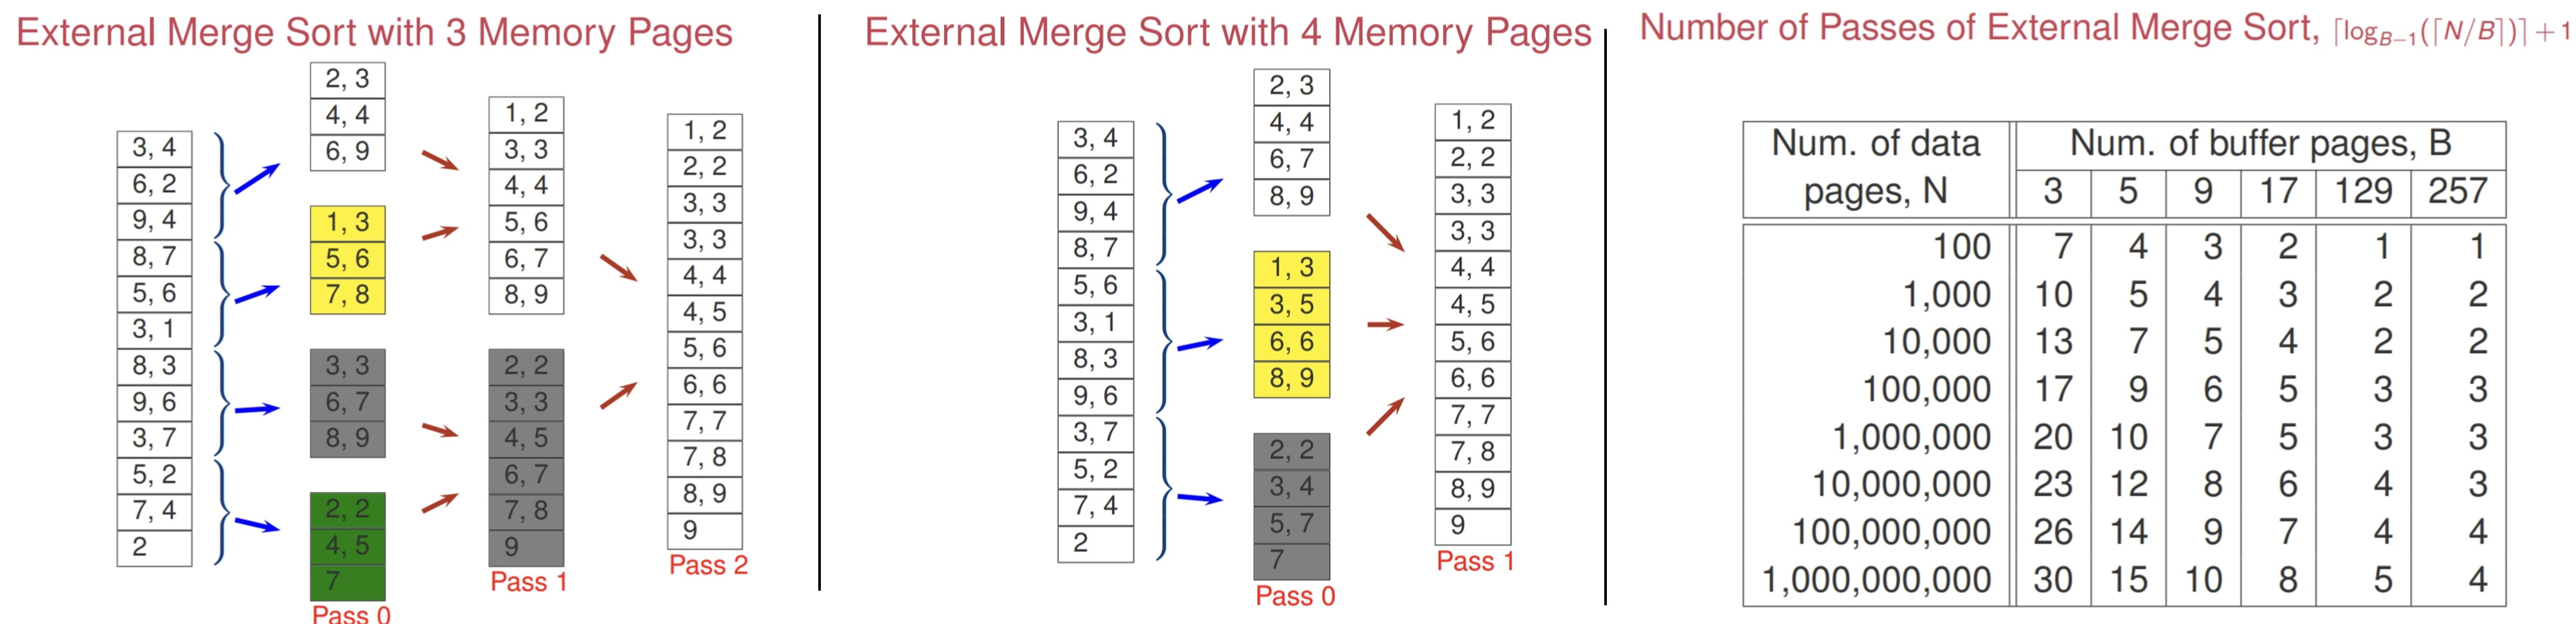
\includegraphics[width = 1\linewidth]{externalMergeSortExample}}
\subsection{External Merge Sort Analysis}
\begin{itemize}
\item \textbf{Note}: We consider only I/O costs, which approx by counting no. of pages read/written as per cost model. (Simple cost model to convey main idea).
\end{itemize}
\centerline{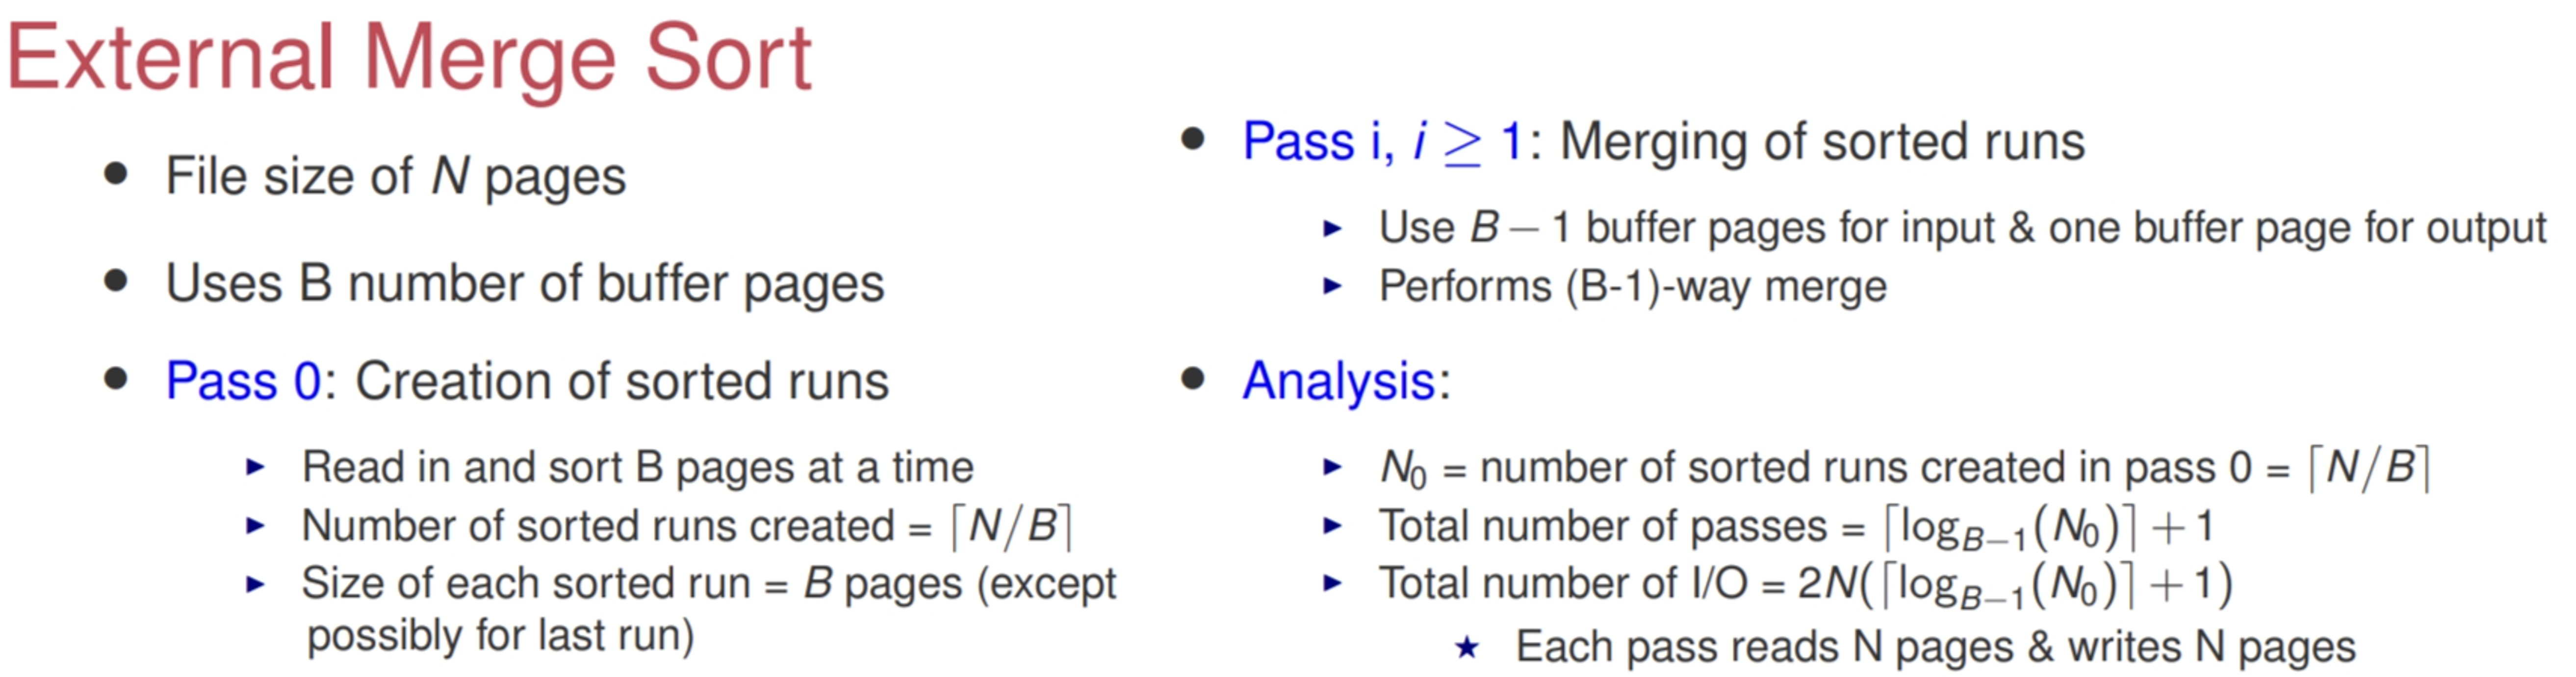
\includegraphics[width = 1\linewidth]{externalMergeSortSummary}}


\subsubsection{External Merge Sort Steps}
\centerline{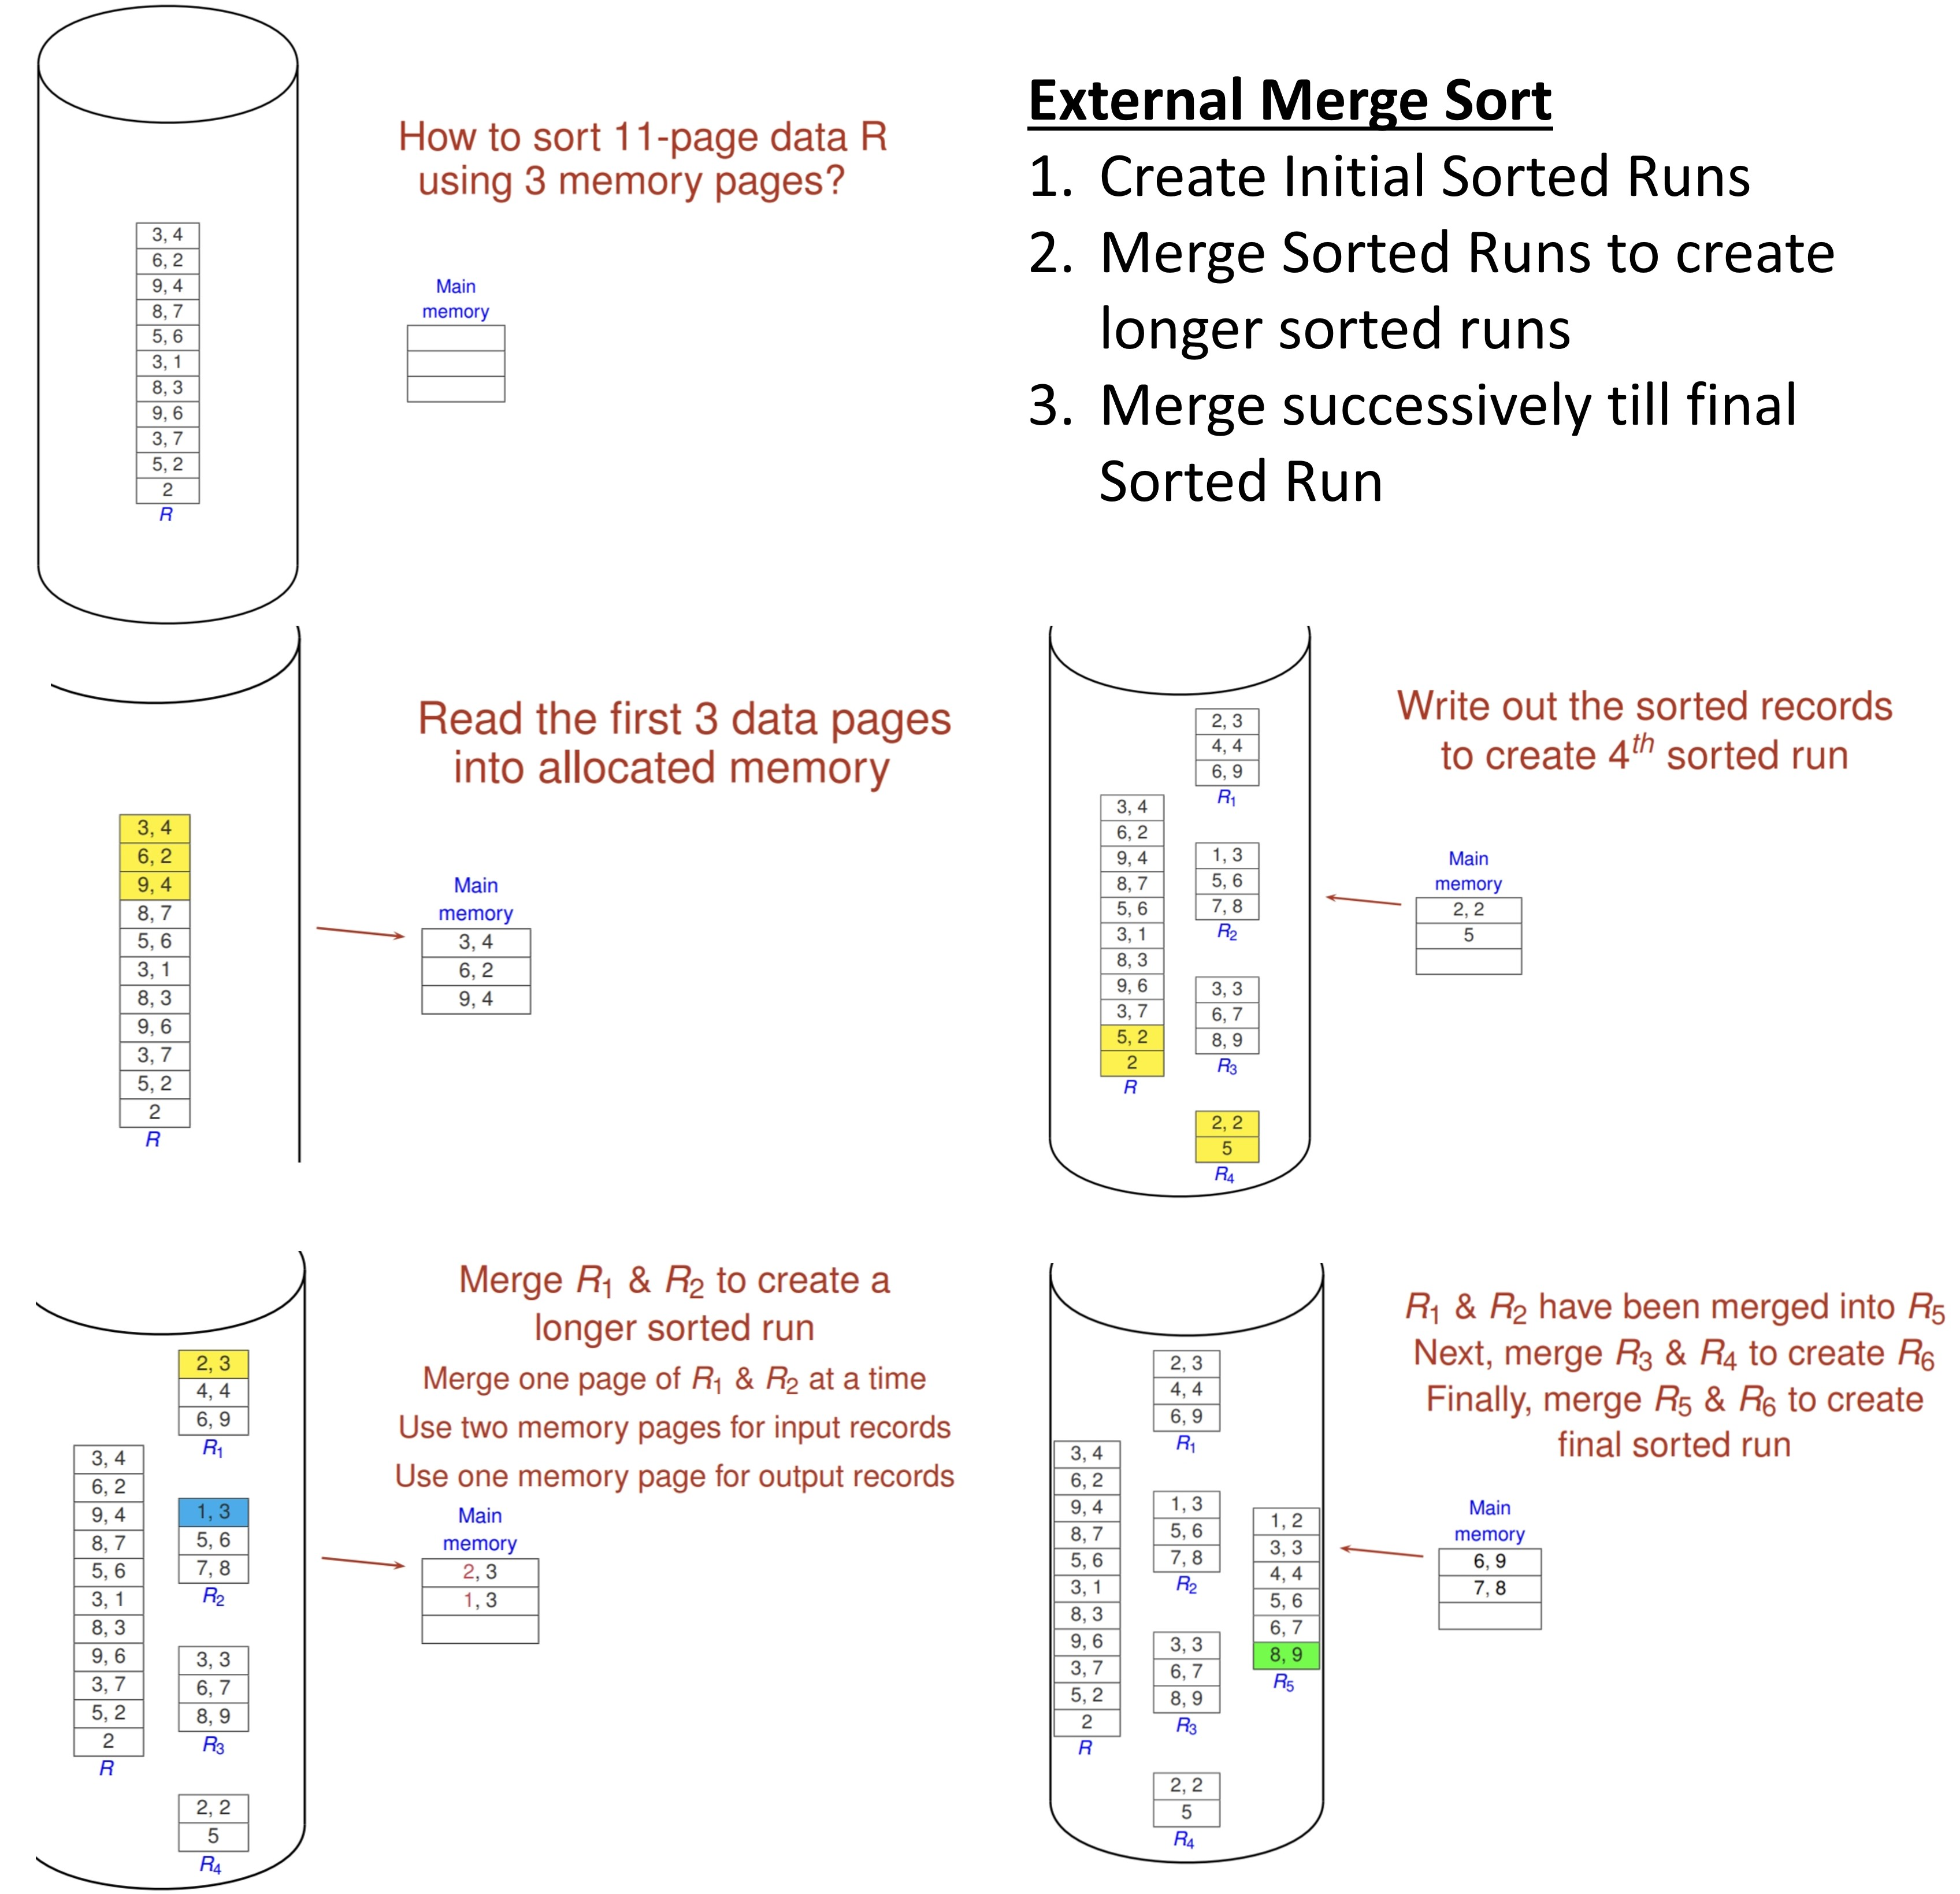
\includegraphics[width = 1\linewidth]{externalMergeSort}}

\columnbreak

\subsection{External Sort Optimization: I/O Cost vs. No. of I/Os}
\begin{itemize}
\item \textbf{Cost Metric}: No. of page I/Os. 
\item Only an approx of true I/O costs, ignores effect of \textbf{block(ed)} I/O, \textbf{single request to read/write several consecutive pages can be cheaper} than read/write same number of pages through independent I/O requests.
\item \textbf{Others}: Consider CPU costs as well, can use \textit{double buffering} to keep CPU busy while I/O op. in progress.
\end{itemize}

\subsection{External Sort, Block(ed) Page I/O Optimization}
\subsubsection{Non-Block(ed) Page I/O}
\begin{itemize}
\item \textbf{Consider only No. of page I/O as metric}: Minimize no. of passes in sorting, as each page in file read and written in each pass. 
\item This means we maximise fan-in \textbf{during merging} (aka, how many runs merged per pass), allocate just one buffer pool page per run, and one buffer page for output of merge.
\item Hence, (B-1)-way merge per run, minimizing number of passes in sorting algorithm.
\end{itemize}

\subsubsection{Block(ed) Page I/O}
\begin{itemize}
\item \textbf{Optimization}: Access in blocks may reduce average cost to read/write single page, consideration to read/write in units of more than one page, or R/W in units of a \textbf{buffer block}.
\item \textbf{Buffer block}, of \textbf{$b$ pages}. \textbf{$B$ is total number of buffer pages} for sorting. 
\end{itemize}
\centerline{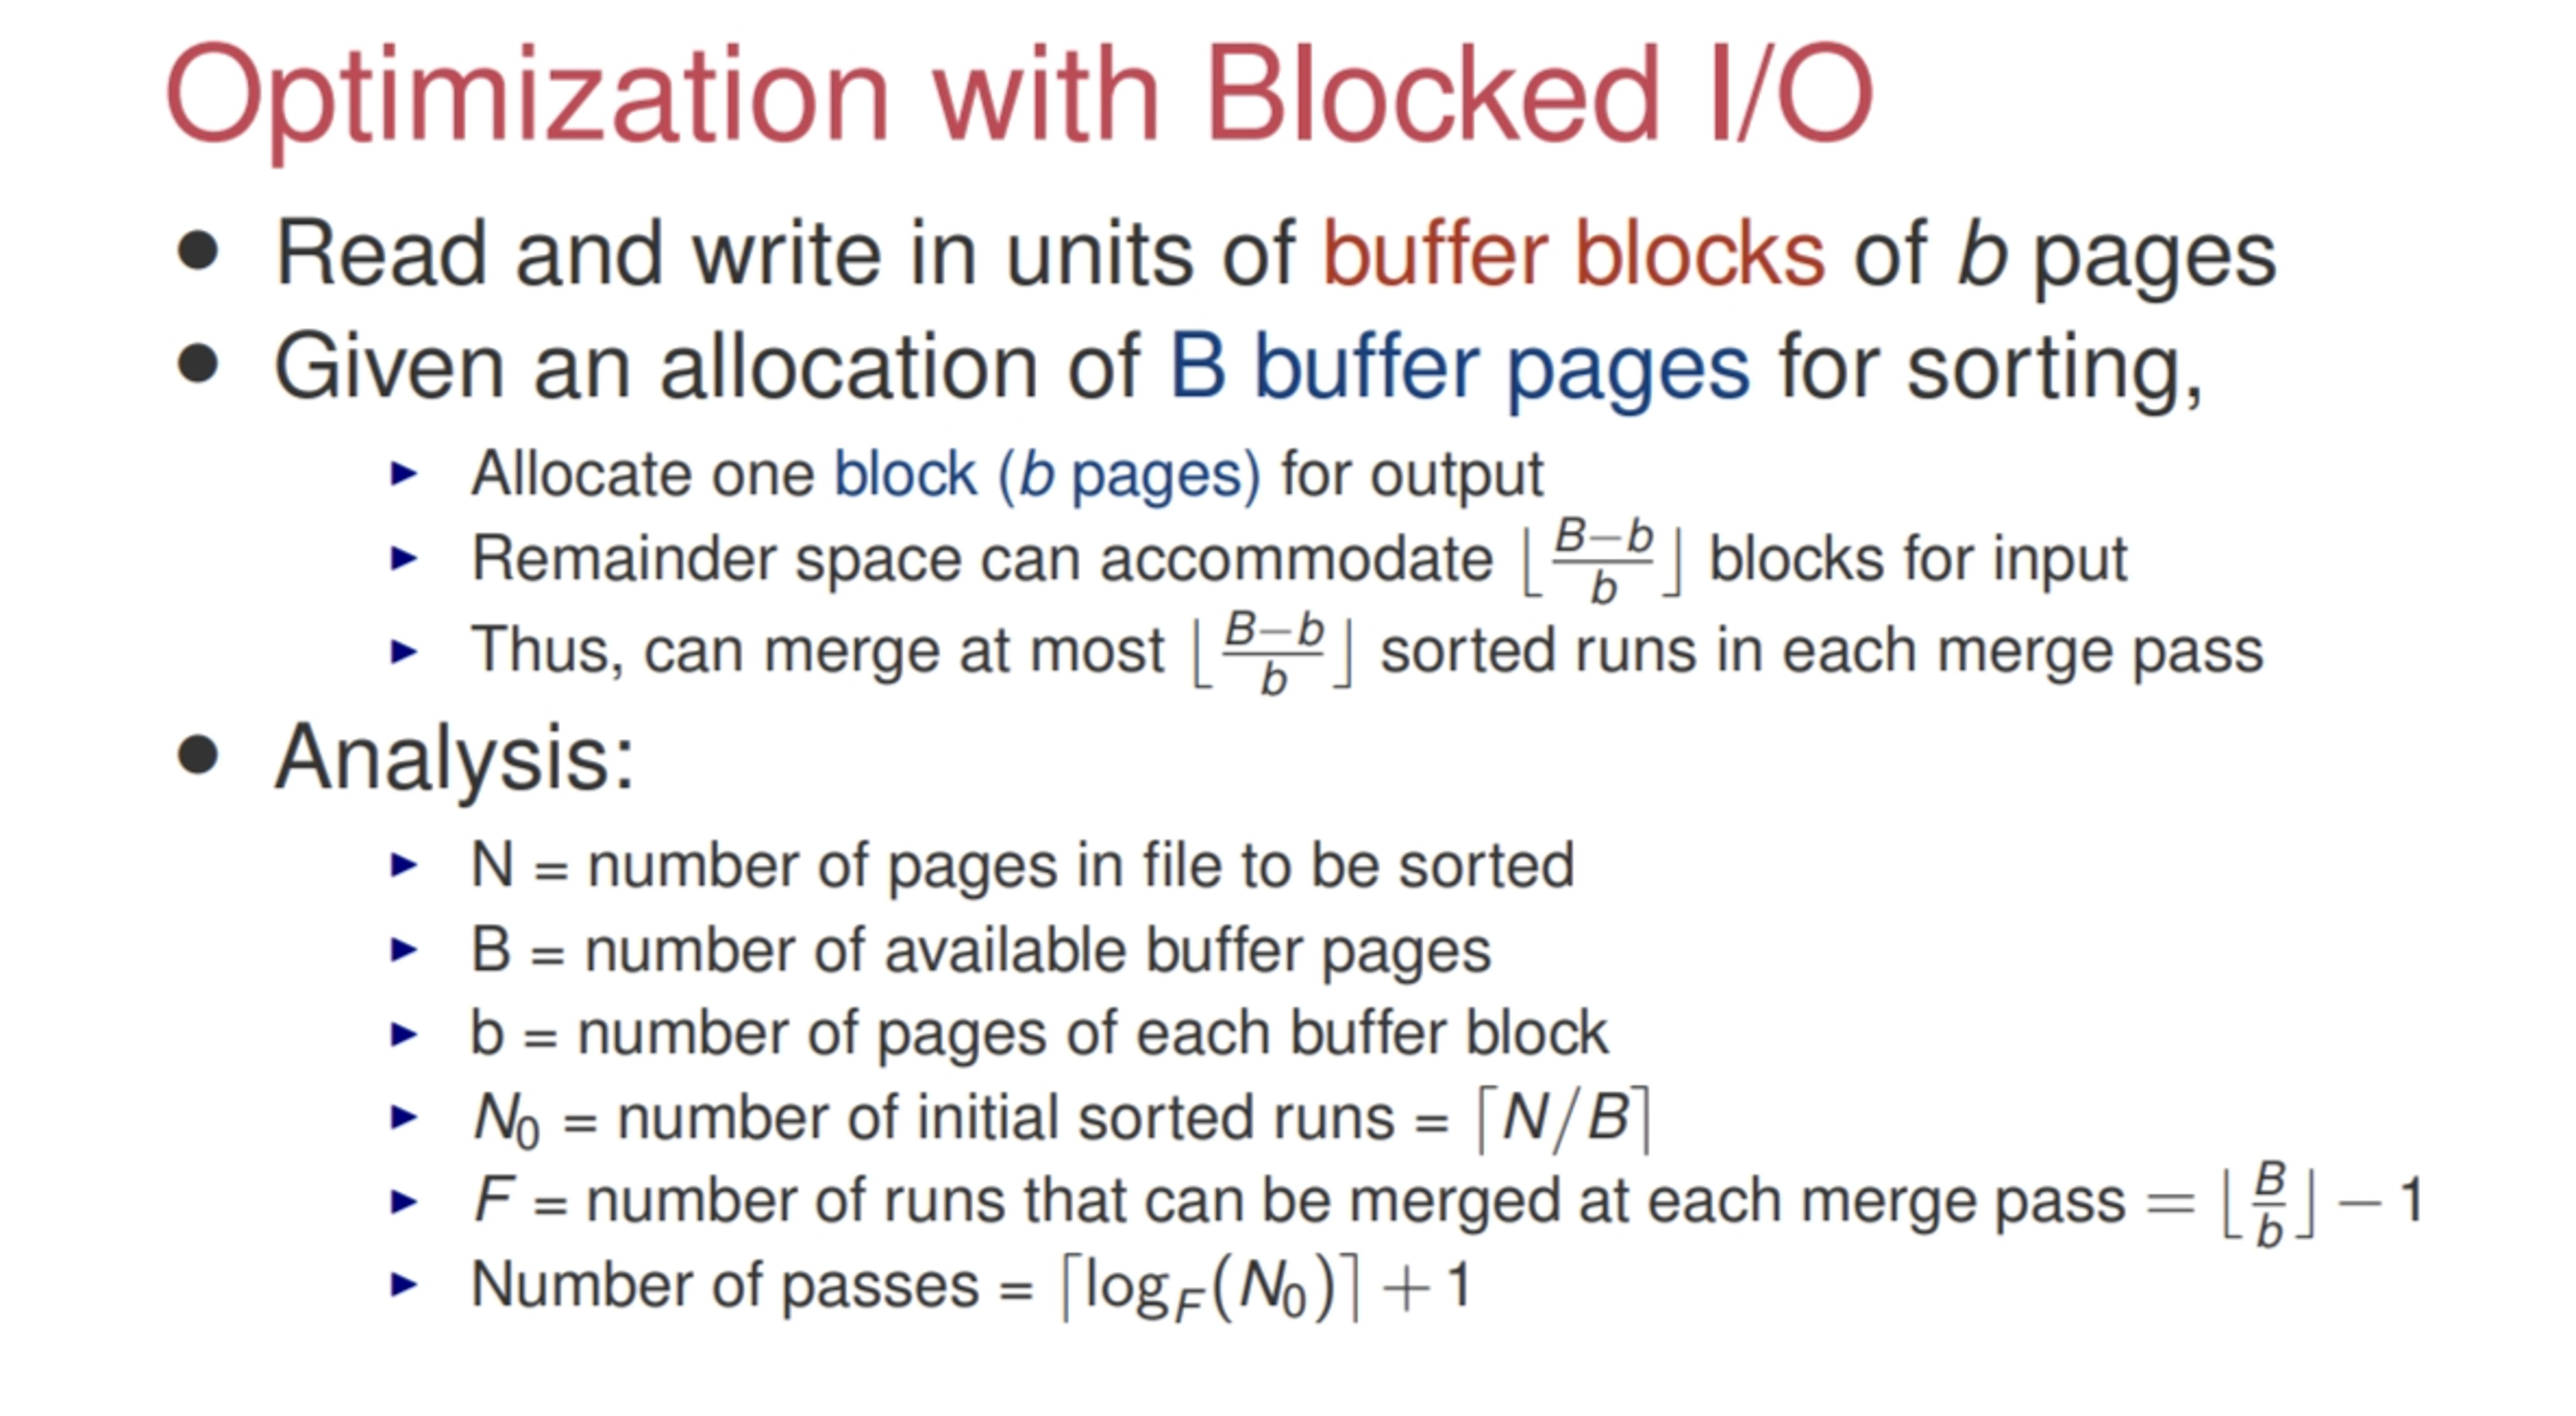
\includegraphics[width = 0.6\linewidth]{blockedIO}}
\begin{itemize}
\item Set aside one buffer block for output of merge. ($B-b$). One buffer block per input run ($\frac{B-b}{b}$). 
\item \textbf{Means can merge} at most floor($\frac{B-b}{b}$) sorted runs in each merge pass.
\end{itemize}
\centerline{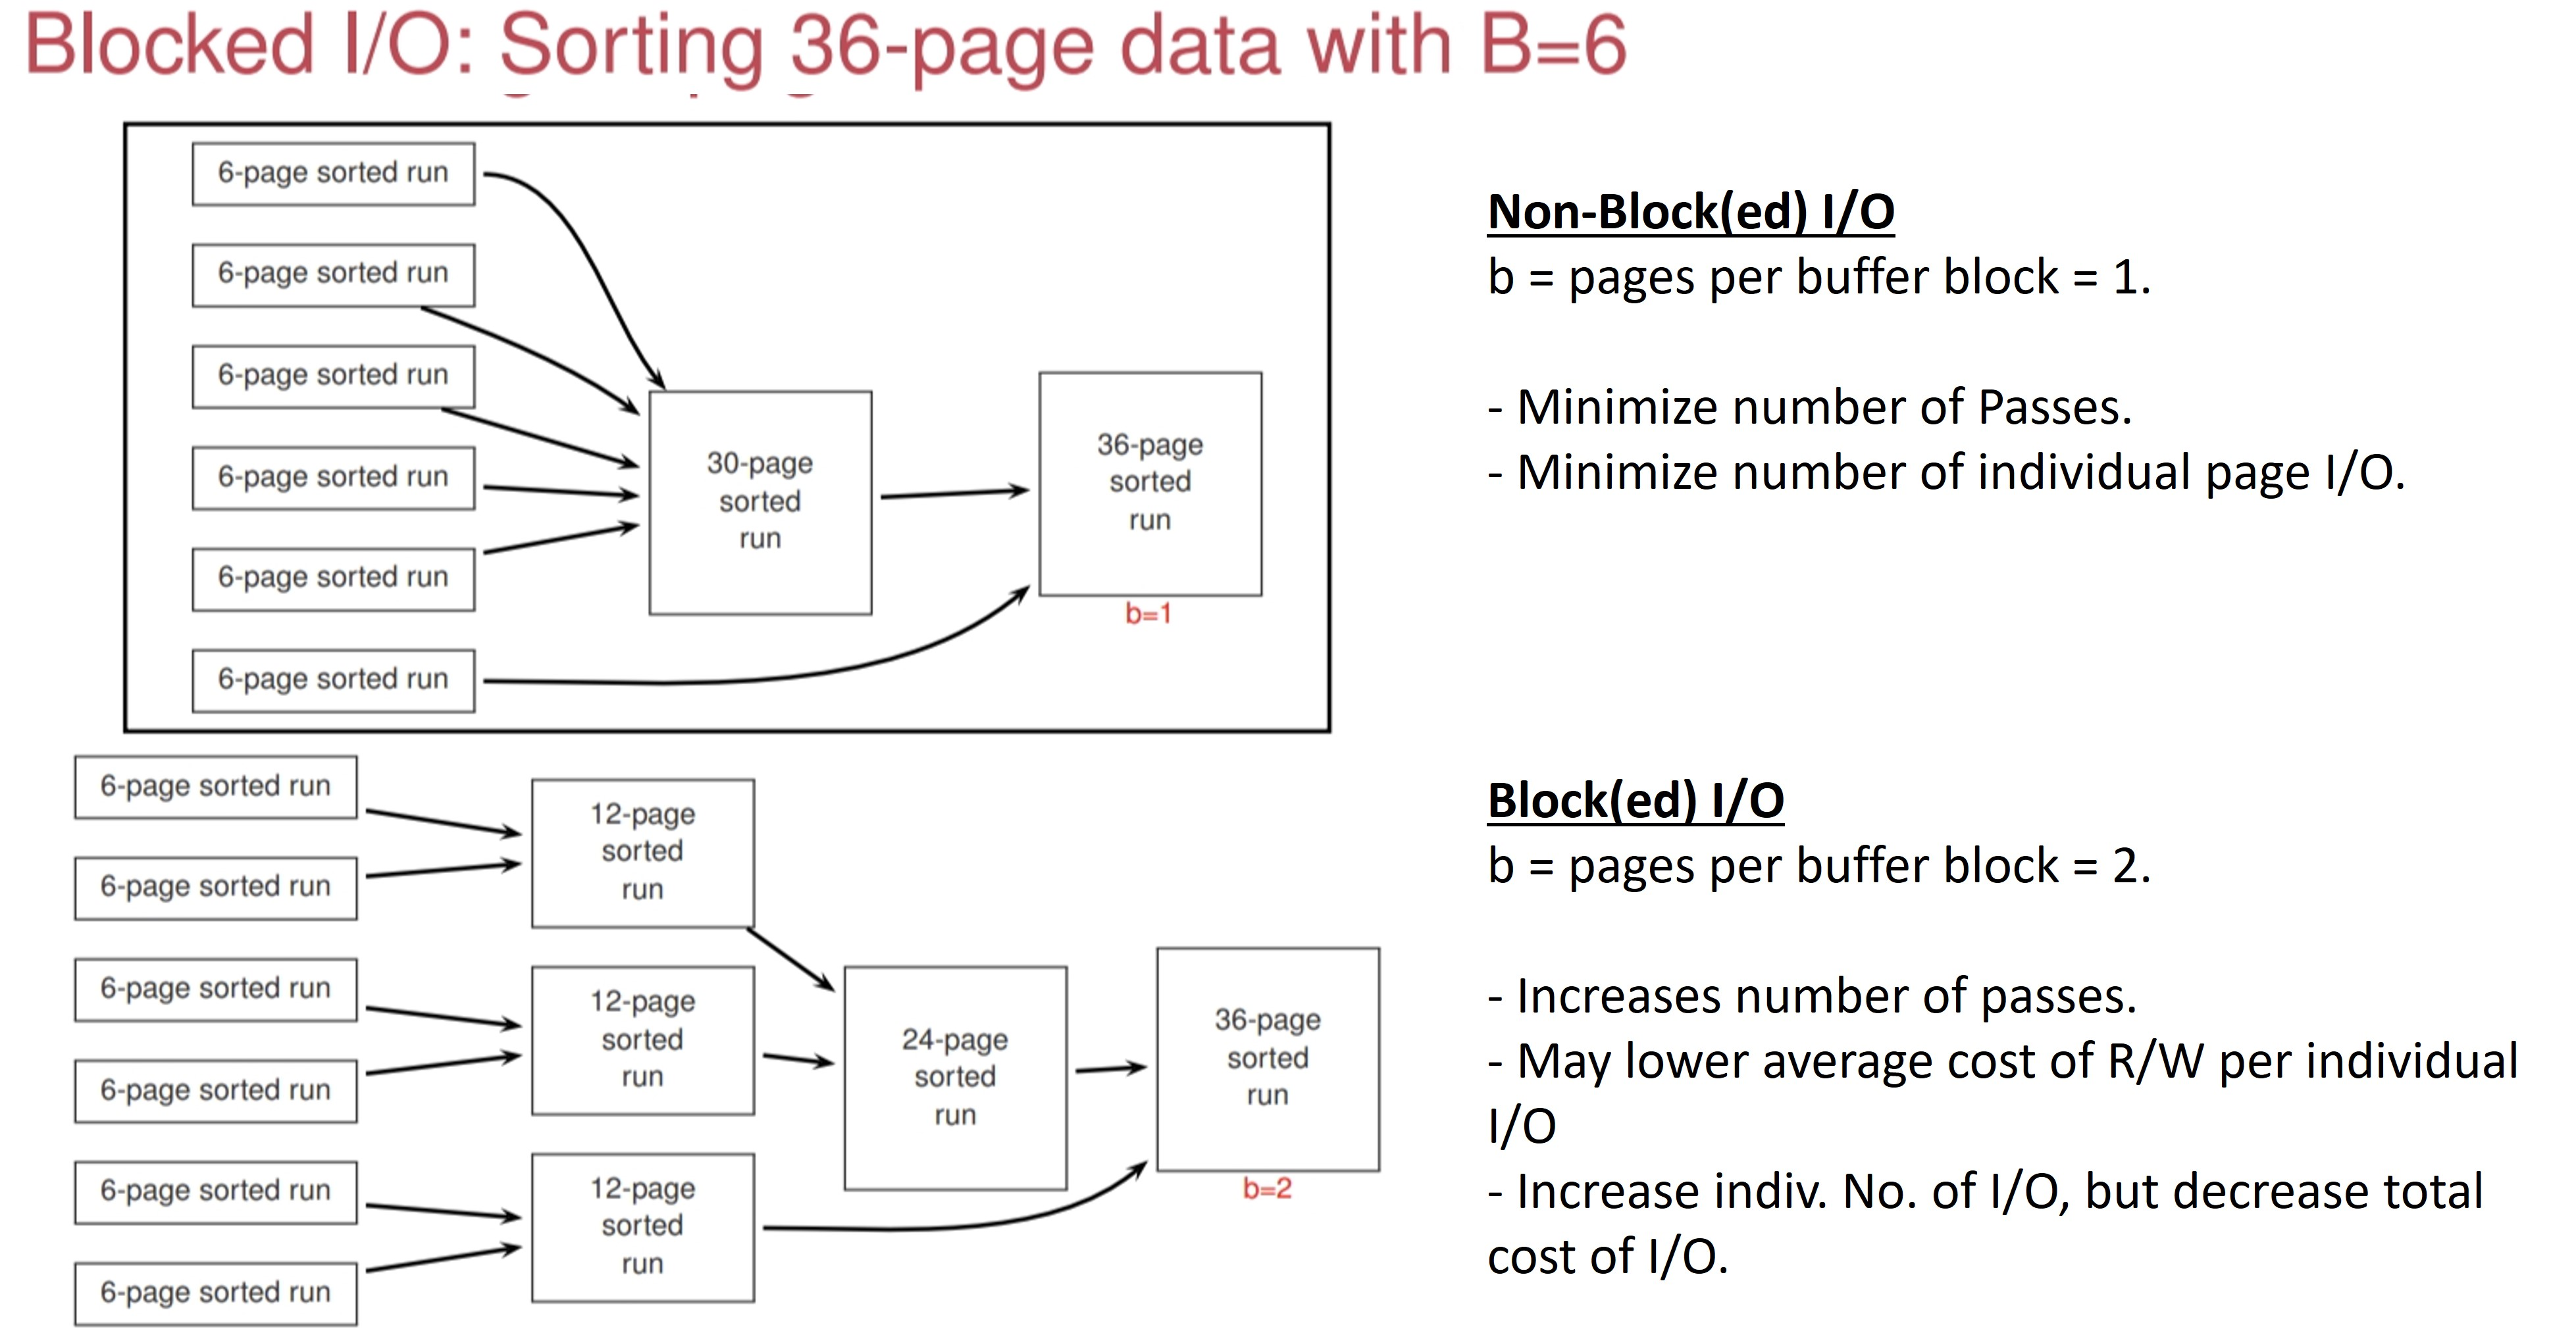
\includegraphics[width = 1\linewidth]{blockedIO2}}
\begin{itemize}
\item \textbf{Overall}: \\
- Larger buffer blocks, (lower average page I/O cost). \\
- But num. passes increase, num page I/O increase. 
\item \textbf{Decrease per-page I/O cost tradeoffs Increase No. of page I/Os.}
\end{itemize}

\columnbreak

\subsection{Sorting using $B^+$-trees}
\begin{itemize}
\item When table to be sorted has existing $B^+$-tree index on sorting attributes.
\begin{itemize}
\item Format 1: Sequentially scan leaf pages of $B^+$-tree.
\item Format 2/3:  Sequentially scan leaf pages of $B^+$-tree.For each leaf page visited, retrieve data records using RIDs.
\end{itemize}
\end{itemize}

\section{Selection $\sigma_p(R)$}
Select rows from Relation $R$ that satisfy selection predicate $p$
\begin{itemize}
\item \textbf{Index Matching}: Index \textbf{matches} selection predicate if index can be used to evaluate it. Consider Hash index, and B+ Tree index.
\end{itemize}

\subsection{Access Path}
\begin{itemize}
\item \textbf{Access path} refers to the given way of accessing data records/entries.
\begin{itemize}
\item \textbf{Table scan}: scan all data pages.
\item \textbf{Index scan}: scan all index pages.
\item \textbf{Index Intersection}: Combine results from multiple index scans (e.g. intersect, union).
\end{itemize}
\item Index scan/intersect follow by \textbf{RID lookups} to retrieve data records.
\end{itemize}

\subsubsection{Selectivity of Access Path}
\centerline{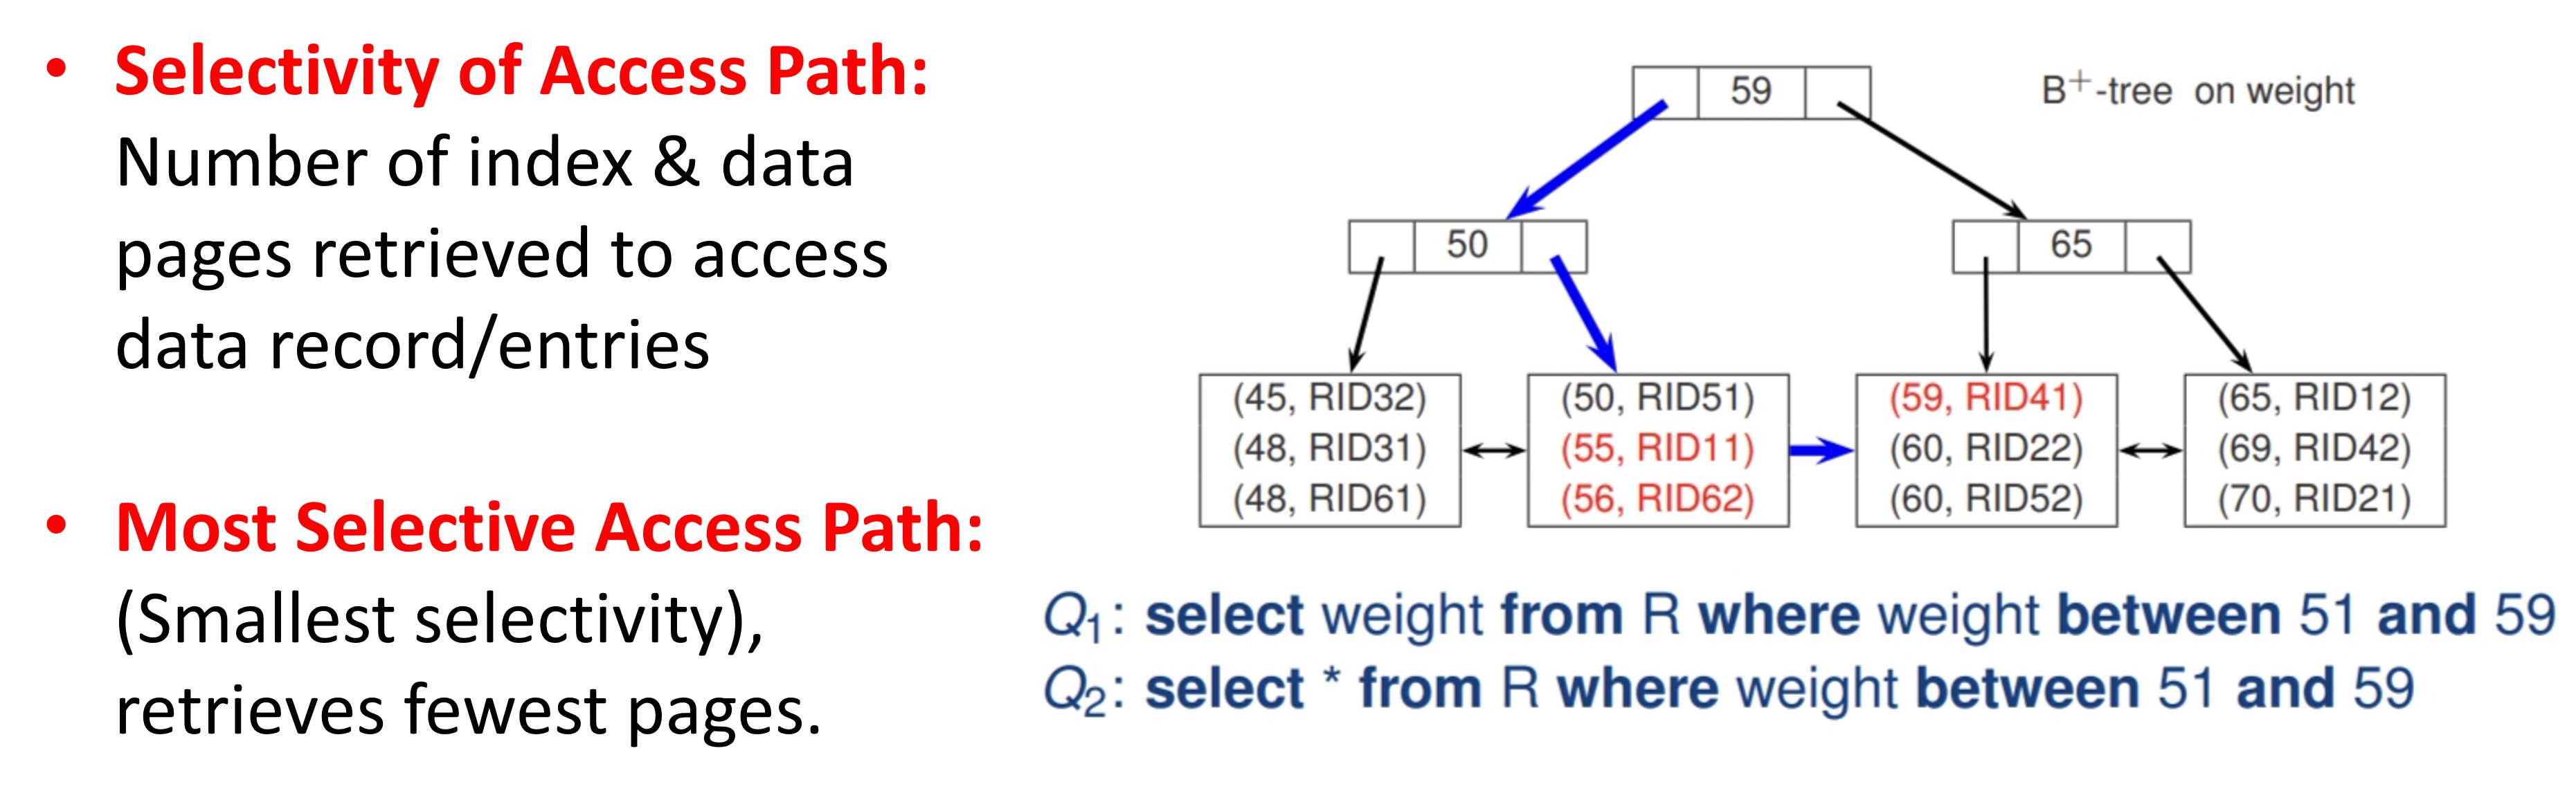
\includegraphics[width = 1\linewidth]{selectivity}}
\begin{itemize}
\item \textbf{Most Selective Access Path minimizes cost of data retrieval.}
\end{itemize}

\subsection{Covering Index}
\centerline{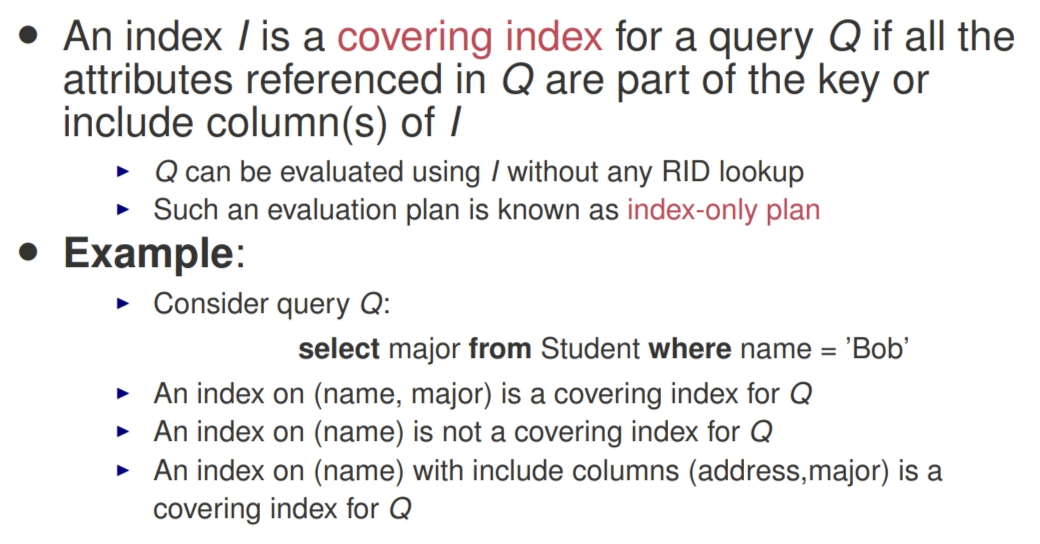
\includegraphics[width = 0.7\linewidth]{coveringIndex}}

\subsubsection{$B^+$-Tree: Include Columns (In Index)}
\centerline{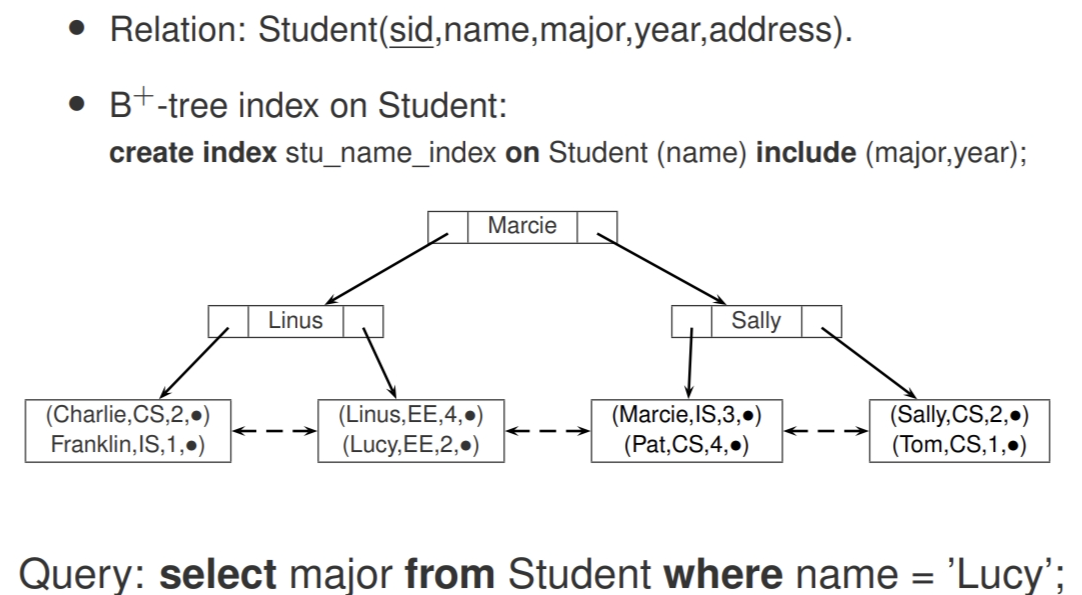
\includegraphics[width = 0.7\linewidth]{includeColumns}}

\subsection{$B^+$-Tree: Selection Evaluation}
\centerline{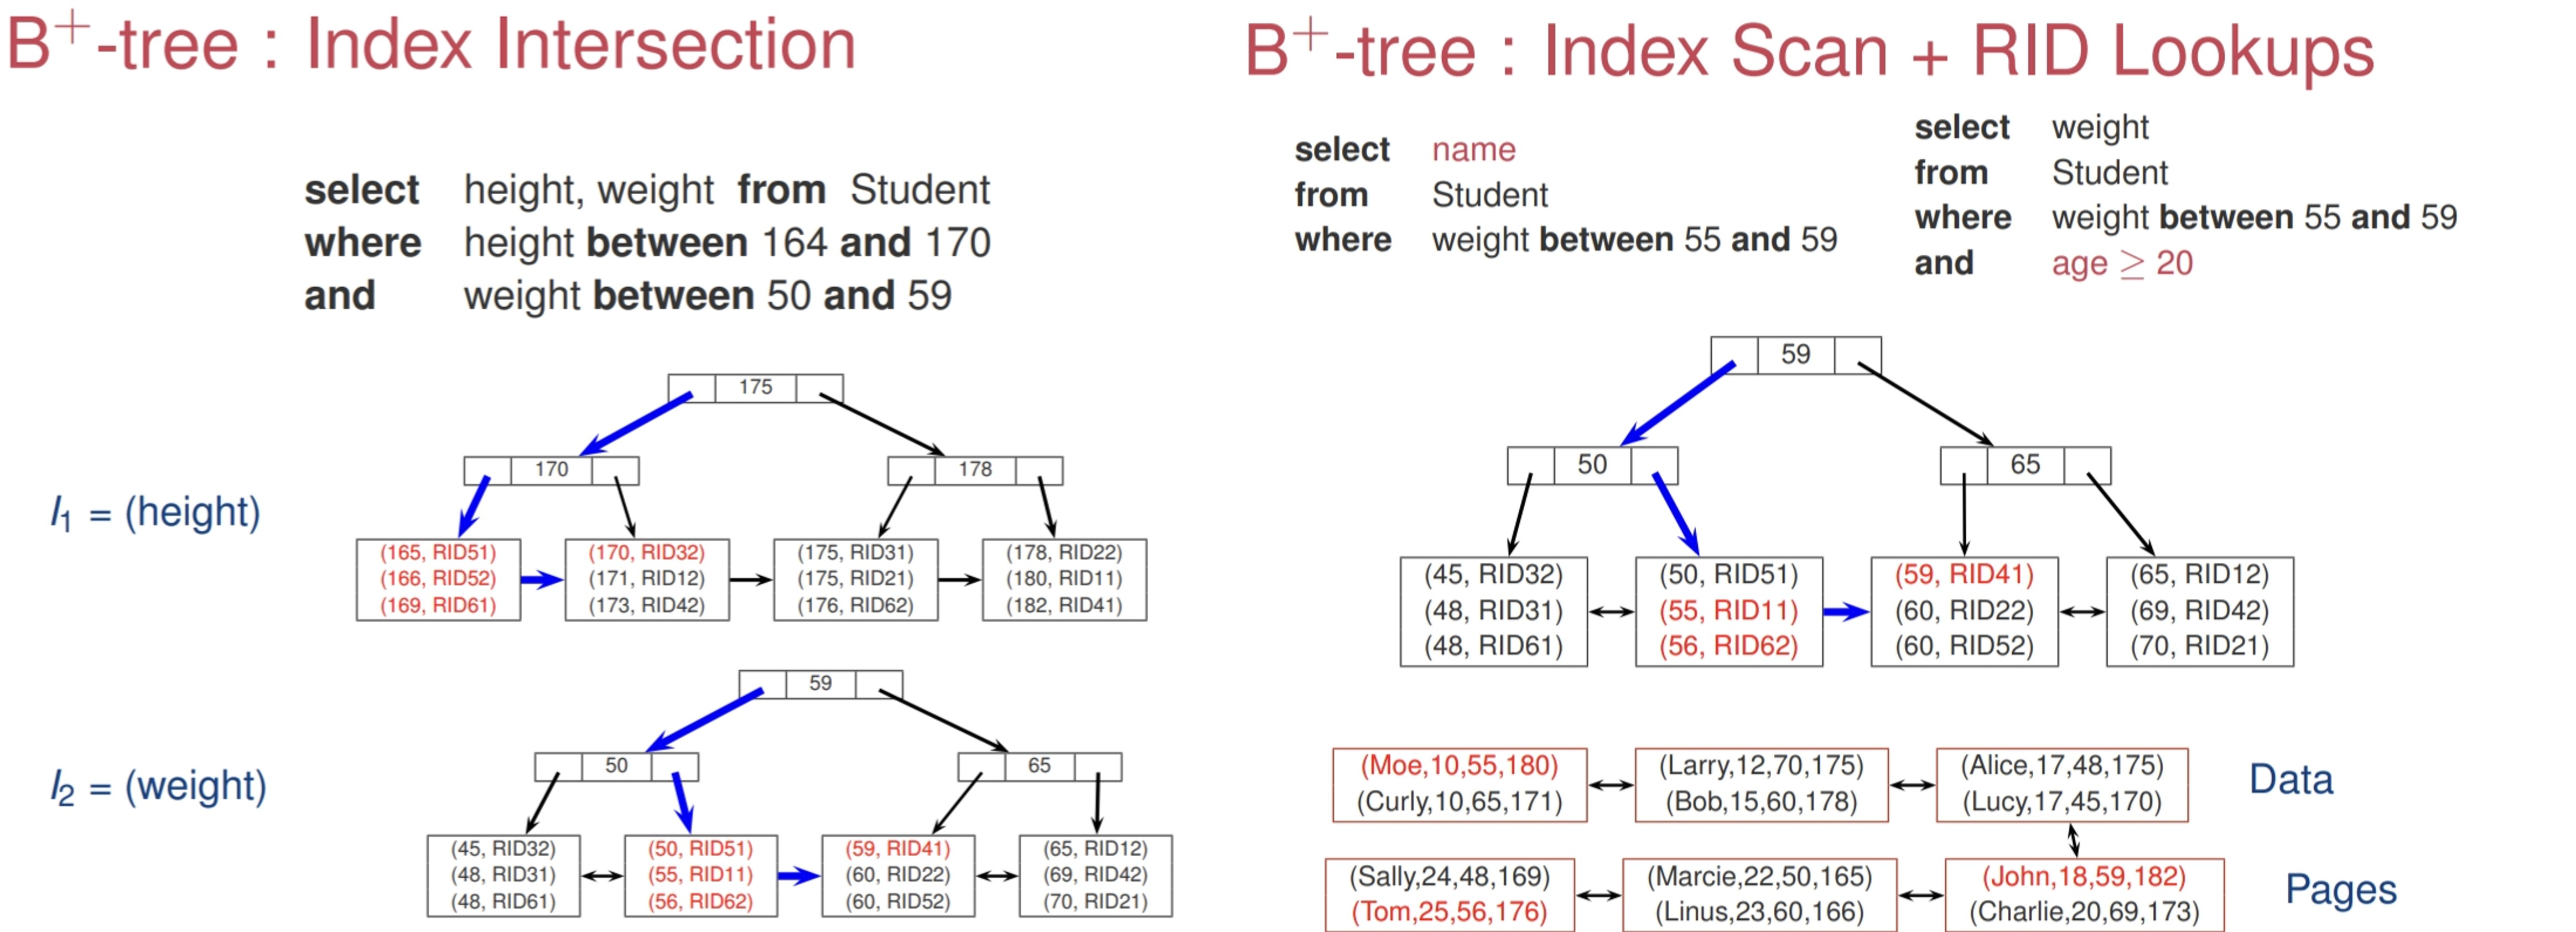
\includegraphics[width = 1\linewidth]{bTreeSelectionEvaluation}}

\subsection{CNF Predicates}
\begin{itemize}
\item \textbf{Selectivity of an access path} depends on primary conjuncts in selection condition (w.r.t. index involved.)
\item Each conjunct acts as filter on table, fraction of tuples satisfying given conjuct called reduction factor.
\end{itemize}

\centerline{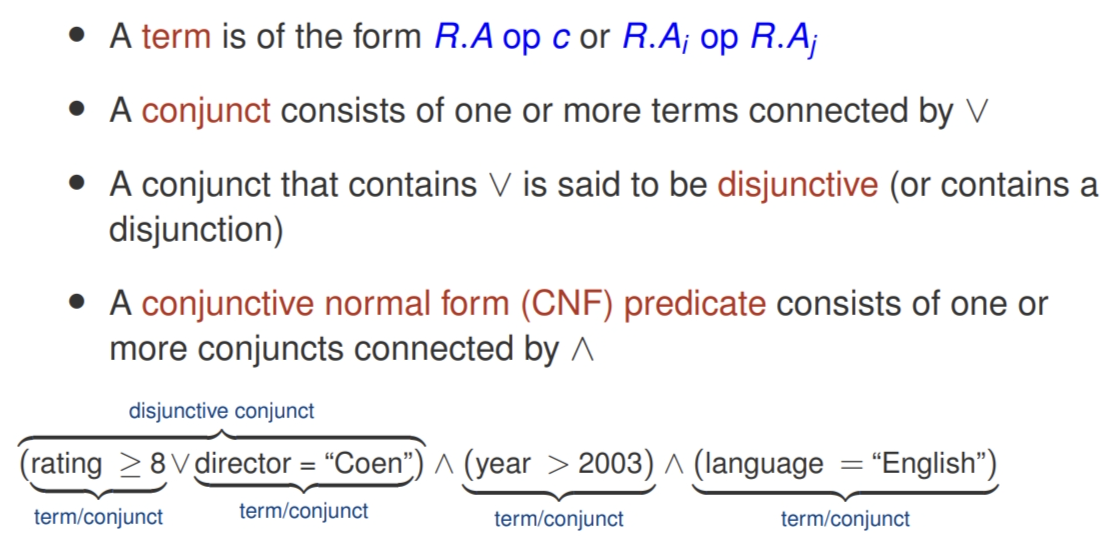
\includegraphics[width = 1\linewidth]{CNF}}
\begin{itemize}
\item \textbf{Non-equality Comparison Operators}: $<, \leq, >, \geq, <>$, between, in.
\end{itemize}

\subsection{Tree Index matching CNF Selection}
\begin{itemize}
\item Determines if Index is useful / appropriate, if index can be used to retrieve just the tuples that satisfy the condition.
\end{itemize}
\centerline{\includegraphics[width = 1\linewidth]{matchingPredicatesTree}}

\subsection{Hash Index matching CNF Selection}
\centerline{\includegraphics[width = 1\linewidth]{matchingPredicatesHash}}

\columnbreak

\subsection{Examples of Index matching CNF Selection}
\centerline{\includegraphics[width = 1\linewidth]{matchingPredicates}}
\medskip

\subsubsection{Primary and Covered Conjuncts}
\begin{itemize}
\item \textbf{Primary Conjuncts}: Subset of conjuncts in selection predicate $p$ that index $I$ \textbf{matches}.
\item In general, only subset of conjuncts of predicate matches index.
\item \textbf{Covered Conjunct}: Conjunct C in predicate $p$ covered if all attributes in $C$ appear in the key, or \textit{include column(s)} of index $I$.
\item Primary conjuncts subset of covered conjuncts.
\end{itemize}

\subsection{Cost of Evaluation of Selection Predicate $p$}

\centerline{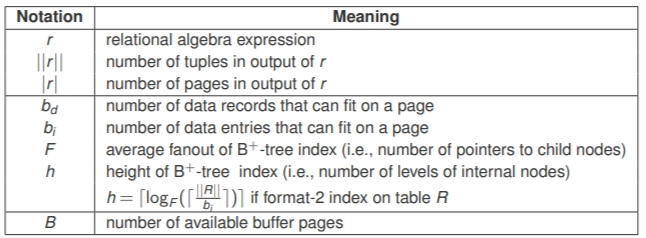
\includegraphics[width = 0.9\linewidth]{notation}}

\subsection{Cost of $B^+$-tree Index Evaluation of $p$}
\centerline{\includegraphics[width = 0.95\linewidth]{BTreeEvaluationCost}}
\centerline{\includegraphics[width = 0.95\linewidth]{BTreeEvaluationCostExample}}

\subsection{Cost of Hash Index Evaluation of $p$}
\centerline{\includegraphics[width = 0.95\linewidth]{hashEvaluationCost}}

\subsection{Evaluating Non-Disjunctive / Disjunctive Conjuncts}
\centerline{\includegraphics[width = 1\linewidth]{Disjunct}}
\begin{itemize}
\item \textbf{Possible strategies to evaluate Disjunctive / Non-Disjunctive predicates}
\item File scan, Use both (fetch RID, take Union), Use B+ tree etc.
\end{itemize}


\end{multicols*}
\end{document}
